\documentclass[11pt,a4paper,twoside,openright]{book}
 
\newcommand{\reporttitle}{Classical Methods in Numerical Analysis Applied to Mathematical Finance: Normal, Lifted, Rough Heston and Pricing Call Options.}
\newcommand{\reportauthor}{Niels D. C. CARIOU KOTLAREK}
\newcommand{\course}{Mean-Variance Porfolio Selection under Volterra Heston model by HAN and WONG}
\newcommand{\professor}{Antoine J. JACQUIER}
\newcommand{\cid}{01831430}
% include file with configuration.


\usepackage[utf8]{inputenc}
\usepackage[T1]{fontenc}

\usepackage[left=2.5cm,right=2.5cm,top=2cm,bottom=3cm]{geometry}%réglages des marges du document selon vos préférences ou celles de votre établissemant
\setlength{\headheight}{15pt}% hauteur de l'entête

\usepackage{array}  %pour les array et binomes de newton 
\usepackage{amsmath,amsfonts,amssymb}%extensions de l'ams pour les mathématiques
\usepackage{amsthm} %pour les théoremes
\usepackage{colortbl}
\usepackage[dvipsnames]{xcolor}
\usepackage{comment} % pour les commentaires
\usepackage{dsfont} %fonction indicatrice
\usepackage{fancybox} %pour shadow box
\usepackage[Rejne]{fncychap}%pour de jolis titres de chapitres voir la doc pour d'autres styles.
\usepackage{fancyhdr}%pour les entêtes et pieds de pages
\usepackage{graphicx}%pour insérer images et pdf entre autres
\graphicspath{{images/}}%pour spécifier le chemin d'accès aux images
\usepackage{lmodern}	%celui ci et le suivant pour les boites
\usepackage{shorttoc}%pour la réalisation d'un sommaire.
\usepackage[most]{tcolorbox}

\usepackage{lipsum} %to test paragraphs
\usepackage{verbatim} %for writing as code
\usepackage{fancyvrb} %this is for reducing size of verbatim
\usepackage{subfig} %for having the figures next to each other
\usepackage{stmaryrd} % pacakge for double brackets, notation for integers.

% packages for tables rotated. and algorithms.
\usepackage[ruled,vlined, linesnumbered]{algorithm2e}
\usepackage{lscape}
\usepackage{rotating}




\usepackage[english]{babel}%pour un document en englais
\usepackage{hyperref}%rend actif les liens, références croisée, toc, ...
		\hypersetup{colorlinks,%
		citecolor=black,%
		filecolor=black,%
		linkcolor=gray,%
		urlcolor=blue} 




		
		
		
%%%%%%%%%%%%%%%%%%%%%%%%%%%%%%%%%%%%%%%%%%%%%%%%%%%%%%%%%%%%%%%%%%%%%%%%%%%%%%%%%%%%%%%%
\makeatletter
\newenvironment{abstract}{%
    \cleardoublepage
    \null\vfil
    \@beginparpenalty\@lowpenalty
    \begin{center}%
      \bfseries \abstractname
      \@endparpenalty\@M
    \end{center}}%
   {\par\vfil\null}
\makeatother


\newenvironment{acknowledgements}{
\renewcommand\abstractname{Acknowledgements}
\begin{abstract}} {\end{abstract}
}


		




%%%%%%%%%%%%%%Remarque
\newtheoremstyle{rq}{}{}{\advance \leftskip2.45cm\relax \itshape}{}
{\bfseries}{}{0pt}{%
\makebox[0pt][r]{%
  \smash{\parbox[t]{3.24cm}{\raggedright\thmname{#1}%
  \thmnumber{\space #2}\thmnote{\newline (#3)}}}%
  \hspace{.5cm}}}
\theoremstyle{rq}
\newtheorem{remarque}{Remark}[chapter]


%%%%%%%%%%%%%%% Définition
\newtheoremstyle{Marine2}% name 
{}% Space above 
{1cm}% Space below 
{\advance \leftskip2.45cm\relax \itshape}% Body font 
{}% Indent amount 
{\bfseries}{}{0pt}
{\makebox[0pt][r]{
  \smash{\parbox[t]{3.25cm}
	    {\raggedright\thmname{#1}%
         \thmnumber{\space #2}\thmnote{\newline 
         \textcolor{BrickRed}{ (#3)}}}}
  	 \hspace{.5cm}}}


\theoremstyle{Marine2}
\newtheorem{definition}{Definition}[section]













\newtcolorbox[auto counter, number within=section]{theoreme}[2][]{%
    colback=white!95!roug,
    colframe=roug,
    colbacktitle=white!80!roug,
    coltitle=black,
    fonttitle=\bfseries, 
    title=Theorem~\thetcbcounter.\ #2,
    enhanced,
    before={\vspace{0.4cm}}, 
    after={\vspace{0.1cm}},
    attach boxed title to top left={yshift=-2mm, xshift=0.4cm},%
    #1% For possible options
}



\tcbset{   
   %%%%%%%%%%%%%%%%%%%%%%%%%%%%%%%%%%%%%%%%%%% EXEMPLES
    SV/.style={
    enhanced,
        breakable,
        sharp corners=all,
        fonttitle=\bfseries\normalsize,
        fontupper=\normalsize\itshape,
        colframe=white,
        before={\vspace{0.2cm}}, 
        after={\vspace{0.2cm}},      
        attach boxed title to top left={xshift=-.232\linewidth, yshift= -7 mm},
        minipage boxed title=.17\linewidth,
        left skip={.12\linewidth},
    coltitle=vert, colback=white!95!vert, colbacktitle=white,
        overlay unbroken ={
            \draw[vert][thick] (title.south west)--(title.south east);
            \draw[vert][thick] ([xshift=3.5mm]frame.north west)--([xshift=3.5mm]frame.south west);},
        overlay first={
            \draw[vert][thick] (title.south west)--(title.south east); 
            \draw[vert][thick] ([xshift=3.5mm]frame.north west)--([xshift=3.5mm]frame.south west);},
        overlay middle={
            \draw[vert][thick] ([xshift=3.5mm]frame.north west)--([xshift=3.5mm]frame.south west);},
        overlay last={
            \draw[vert][thick] ([xshift=3.5mm]frame.north west)--([xshift=3.5mm]frame.south west);},
        },
        %%%%%%%%%%%%%%%%%%%%%%%%%%%%%%%%%%% EXERCICES DE COMPREHENSION
    SO/.style={
    enhanced,
        breakable,
        sharp corners=all,
        fonttitle=\bfseries\normalsize,
        fontupper=\normalsize\itshape,
        colframe=white,
        before={\vspace{0.1cm}}, 
        after={\vspace{0.3cm}},      
         attach boxed title to top left,
        boxed title style={empty, size=minimal, bottom=1.5mm},
    coltitle=oran, colback=white!95!oran, colbacktitle=white,
        overlay unbroken ={
            \draw[oran][thick] (title.south west)--(title.south east);
            \draw[oran][thick] ([xshift=3.5mm]frame.north west)--([xshift=3.5mm]frame.south west);},
        overlay first={
            \draw[oran][thick] (title.south west)--(title.south east); 
            \draw[oran][thick] ([xshift=3.5mm]frame.north west)--([xshift=3.5mm]frame.south west);},
        overlay middle={
            \draw[oran][thick] ([xshift=3.5mm]frame.north west)--([xshift=3.5mm]frame.south west);},
        overlay last={
            \draw[oran][thick] ([xshift=3.5mm]frame.north west)--([xshift=3.5mm]frame.south west);},
        },   
                %%%%%%%%%%%%%%%%%%%%%%%%%%%%%%%%%%% EXERCICES DE ANNONCES
    SO*/.style={
    enhanced,
        breakable,
        sharp corners=all,
        fonttitle=\bfseries\normalsize,
        fontupper=\normalsize\itshape,
        colframe=white,
        before={\vspace{0.2cm}}, 
        after={\vspace{0.2cm}},      
        attach boxed title to top left={xshift=-.232\linewidth, yshift= -7 mm},
        minipage boxed title=.17\linewidth,
        left skip={.12\linewidth},
    coltitle=oran, colback=white!95!oran, colbacktitle=white,
        overlay unbroken ={
            \draw[oran][thick] (title.south west)--(title.south east);
            \draw[oran][thick] ([xshift=3.5mm]frame.north west)--([xshift=3.5mm]frame.south west);},
        overlay first={
            \draw[oran][thick] (title.south west)--(title.south east); 
            \draw[oran][thick] ([xshift=3.5mm]frame.north west)--([xshift=3.5mm]frame.south west);},
        overlay middle={
            \draw[oran][thick] ([xshift=3.5mm]frame.north west)--([xshift=3.5mm]frame.south west);},
        overlay last={
            \draw[oran][thick] ([xshift=3.5mm]frame.north west)--([xshift=3.5mm]frame.south west);},
        },   
        %%%%%%%%%%%%%%%%%%%%%%%%%%%%%%%%%%%%%%%% DEMONSTRATION
    SQ/.style={
        enhanced,
        breakable,
        sharp corners=all,
        fonttitle=\bfseries\normalsize,
        fontupper=\normalsize\itshape,
        colframe=white,
        colback=white!95!viol, 
        colbacktitle=white,
        coltitle=viol, 
        before={\vspace{0.1cm}}, 
        after={\vspace{0.8cm}},      
        attach boxed title to top left={xshift=-.23\linewidth, yshift= -11 mm}, % xshift, how much you shift title in comparison to the box
        minipage boxed title=.155\linewidth,
        after upper={\hfill$\qed$},
        left skip={.19\linewidth}, % this changes how far you put the title
        overlay unbroken ={
            \draw[viol][thick] (title.south west)--(title.south east);
            \draw[viol][thick] ([xshift=3.5mm]frame.north west)|-([xshift=15mm]frame.south west);},
        overlay first={
            \draw[viol][thick] (title.south west)--(title.south east); 
            \draw[viol][thick] ([xshift=3.5mm]frame.north west)--([xshift=3.5mm]frame.south west);},
        overlay middle={
            \draw[viol][thick] ([xshift=3.5mm]frame.north west)--([xshift=3.5mm]frame.south west);},
        overlay last={
            \draw[viol][thick] ([xshift=3.5mm]frame.north west)|-([xshift=15mm]frame.south west);},
    },
    %%%%%%%%%%%%%%%%%%%%%%%%%%%%%%%%%%%%%%% EXERCICES DENTRAINEMENT 
    ST/.style={
    enhanced,
        breakable,
        sharp corners=all,
        fonttitle=\bfseries\normalsize,
        fontupper=\normalsize\itshape,
        colframe=white,
        before={\vspace{0.1cm}}, 
        after={\vspace{0.3cm}},      
        attach boxed title to top left,
        boxed title style={empty, size=minimal, bottom=1.5mm},
    coltitle=oran, colback=white, colbacktitle=white,
        overlay unbroken ={
            \draw[oran][thick] (title.south west)--(title.south east);
            \draw[oran][thick] ([xshift=3.5mm]frame.north west)--([xshift=3.5mm]frame.south west);},
        overlay first={
            \draw[oran][thick] (title.south west)--(title.south east); 
            \draw[oran][thick] ([xshift=3.5mm]frame.north west)--([xshift=3.5mm]frame.south west);},
        overlay middle={
            \draw[oran][thick] ([xshift=3.5mm]frame.north west)--([xshift=3.5mm]frame.south west);},
        overlay last={
            \draw[oran][thick] ([xshift=3.5mm]frame.north west)--([xshift=3.5mm]frame.south west);},
        },   
        %%%%%%%%%%%%%%%%%%%%%%%%%%%%%%%%%%%%%%%%%%% SOLUTIONS
    SS/.style={
    enhanced,
        breakable,
        sharp corners=all,
        fonttitle=\bfseries\normalsize,
        fontupper=\normalsize\itshape,
        colframe=white,
        before={\vspace{0.1cm}}, 
        after={\vspace{0.3cm}}, 
        attach boxed title to top left,
        boxed title style={empty, size=minimal, bottom=1.5mm},     
        after upper={\hfill$\qed$},
    coltitle=mauv, colback=white!95!mauv, colbacktitle=white,
        overlay unbroken ={
            \draw[mauv][thick] (title.south west)--(title.south east);
            \draw[mauv][thick] ([xshift=3.5mm]frame.north west)|-([xshift=15mm]frame.south west);
        },
        overlay first={
            \draw[mauv][thick] (title.south west)--(title.south east); 
            \draw[mauv][thick] ([xshift=3.5mm]frame.north west)--([xshift=3.5mm]frame.south west);},
        overlay middle={
            \draw[mauv][thick] ([xshift=3.5mm]frame.north west)--([xshift=3.5mm]frame.south west);},
        overlay last={
            \draw[mauv][thick] ([xshift=3.5mm]frame.north west)|-([xshift=15mm]frame.south west);
            },
    },  
        %%%%%%%%%%%%%%%%%%%%%%%%%%%%%%%%%%%%%%%%%%% SOLUTIONS
    SSE/.style={
    enhanced,
        breakable,
        sharp corners=all,
        fonttitle=\bfseries\normalsize,
        fontupper=\normalsize\itshape,
        colframe=white,
        before={\vspace{0.1cm}}, 
        after={\vspace{0.3cm}},      
 attach boxed title to top left,
        boxed title style={empty, size=minimal, bottom=1.5mm},
    coltitle=mauv, colback=white, colbacktitle=white,
        overlay unbroken ={
            \draw[mauv][thick] (title.south west)--(title.south east);
            \draw[mauv][thick] ([xshift=3.5mm]frame.north west)|-([xshift=15mm]frame.south west);
            },
        overlay first={
            \draw[mauv][thick] (title.south west)--(title.south east); 
            \draw[mauv][thick] ([xshift=3.5mm]frame.north west)--([xshift=3.5mm]frame.south west);},
        overlay middle={
            \draw[mauv][thick] ([xshift=3.5mm]frame.north west)--([xshift=3.5mm]frame.south west);},
        overlay last={
            \draw[mauv][thick] ([xshift=3.5mm]frame.north west)|-([xshift=15mm]frame.south west);
            },
    },  
}





\newtcbtheorem[auto counter, number within=section]{ajoutationV}{Example}{SV}{theo}
\newtcbtheorem[auto counter, number within=section]{demo}{Proof}{SQ}{theo}

%---------------------------------

\newtcolorbox[auto counter, number within=chapter]{entrainement}[2][]{title={\hypertarget{exer:#2}{Entrainement \thetcbcounter.\hfill\hyperlink{sol:#2}{Solution}}},#1, ST}

\newtcolorbox[auto counter, number within=chapter]{soluENT}[2][]{title={\hypertarget{sol:#2}{Correction \thetcbcounter.\hfill\hyperlink{exer:#2}{Exercise}}},#1, SSE}

%---------------------------------

\newtcolorbox[use counter from=entrainement, number within=chapter]{ajoutationO}[2][]{title={\hypertarget{exer:#2}{Exercice \thetcbcounter.\hfill\hyperlink{sol:#2}{Solution}}},#1, SO}

\newtcolorbox[use counter from=soluENT, number within=chapter]{solu}[2][]{title={\hypertarget{sol:#2}{Solution \thetcbcounter.\hfill\hyperlink{exer:#2}{Exercice}}},#1, SS}



%annonce d'exos

\newtcbtheorem[auto counter, number within=chapter]{ajoutationO*}{Exercices}{SO*}{theo}


%%%%%%%%%%%%%% change fontsize and properties of titles	%%%%%%%%%%%%%%%%%%%%%%%%%%%%%%%%%%

\usepackage{titlesec} %pour redéfinir les headers

\newcommand{\sectionbreak}{\clearpage}

\titleformat{\section}
{\Large\bfseries\color[RGB]{10, 80, 144}}
{\textcolor[RGB]{10, 80, 144}{~ \thesection}}
{1em}{}

\titleformat{\subsection}
{\large\bfseries}
{\rlap{\color[RGB]{238,243,252}\rule[-1.25ex]{\textwidth}{4ex}}\textcolor{Black}{~ \thesubsection}}
{1em}{}
% Alice blue (240, 248, 255)

\titleformat*{\subsubsection}{\large\bfseries}
\titleformat*{\paragraph}{\large\bfseries}
\titleformat*{\subparagraph}{\large\bfseries}


\titlespacing*{\subsection}
{0pt}{10mm}{7mm}







%%%%%%%%%%%%%%%%%%%style front%%%%%%%%%%%%%%%%%%%%%%%%%%%%%%%%%%%%%%%%%	
	\fancypagestyle{front}{%
  		\fancyhf{}%on vide les entêtes
  		\fancyfoot[C]{page \thepage}%
  		\renewcommand{\headrulewidth}{0pt}%trait horizontal pour l'entête
  		\renewcommand{\footrulewidth}{0.4pt}%trait horizontal pour les pieds de pages
  		}


%%%%%%%%%%%%%%%%%%%style main%%%%%%%%%%%%%%%%%%%%%%%%%%%%%%%%%%%%
	\fancypagestyle{main}{%
		\fancyhf{}
  		\renewcommand{\chaptermark}[1]{\markboth{\chaptername\ \thechapter.\ ##1}{}}% redéfintion pour avoir ici les titres des chapitres des sections en minuscules
  		\renewcommand{\sectionmark}[1]{\markright{\thesection\ ##1}}
		\fancyhead[c]{}
		\fancyhead[RO,LE]{\rightmark}%
  		\fancyhead[LO,RE]{\leftmark}
		\fancyfoot[C]{}
		\fancyfoot[RO,LE]{page \thepage}%
  		\fancyfoot[LO,RE]{contact : niels.carioukotlarek@yahoo.com}
  		}


%%%%%%%%%%%%%%%%%%%style back%%%%%%%%%%%%%%%%%%%%%%%%%%%%%%%%%%%%%%%%%	
	\fancypagestyle{back}{%
  		\fancyhf{}%on vide les entêtes
  		\fancyfoot[C]{page \thepage}%
  		\renewcommand{\headrulewidth}{0pt}%trait horizontal pour l'entête
  		\renewcommand{\footrulewidth}{0.4pt}%trait horizontal pour les pieds de pages
		}






%%%%%=======================================================================tikz
\usepackage{tikz}
\usetikzlibrary{arrows.meta}
\usepackage{mathdots}
\usepackage{mathtools}
\usepackage{pdflscape}
\usepackage{pgfplots}
\usepackage{siunitx}
\usepackage{slashed}
\usepackage{tabularx}
\usepackage{tikz}
\usepackage{tkz-euclide}
\usepackage[normalem]{ulem}
\usepackage[all]{xy}
\usepackage{imakeidx}



\pgfarrowsdeclarecombine{twolatex'}{twolatex'}{latex'}{latex'}{latex'}{latex'}
\tikzset{->>/.style = {decoration={markings,
                                  mark=at position 1 with {\arrow[scale=2]{latex'}}},
                      postaction={decorate}}}
\tikzset{<-/.style = {decoration={markings,
                                  mark=at position 0 with {\arrowreversed[scale=2]{latex'}}},
                      postaction={decorate}}}
\tikzset{<->/.style = {decoration={markings,
                                   mark=at position 0 with {\arrowreversed[scale=2]{latex'}},
                                   mark=at position 1 with {\arrow[scale=2]{latex'}}},
                       postaction={decorate}}}
\tikzset{->-/.style = {decoration={markings,
                                   mark=at position #1 with {\arrow[scale=2]{latex'}}},
                       postaction={decorate}}}
\tikzset{-<-/.style = {decoration={markings,
                                   mark=at position #1 with {\arrowreversed[scale=2]{latex'}}},
                       postaction={decorate}}}
\tikzset{<<-/.style = {decoration={markings,
                                  mark=at position 0 with {\arrowreversed[scale=2]{twolatex'}}},
                      postaction={decorate}}}
\tikzset{<<->>/.style = {decoration={markings,
                                   mark=at position 0 with {\arrowreversed[scale=2]{twolatex'}},
                                   mark=at position 1 with {\arrow[scale=2]{twolatex'}}},
                       postaction={decorate}}}
\tikzset{->>-/.style = {decoration={markings,
                                   mark=at position #1 with {\arrow[scale=2]{twolatex'}}},
                       postaction={decorate}}}
\tikzset{-<<-/.style = {decoration={markings,
                                   mark=at position #1 with {\arrowreversed[scale=2]{twolatex'}}},
                       postaction={decorate}}}

\tikzset{circ/.style = {fill, circle, inner sep = 0, minimum size = 3}}
\tikzset{scirc/.style = {fill, circle, inner sep = 0, minimum size = 1.5}}
\tikzset{mstate/.style={circle, draw, blue, text=black, minimum width=0.7cm}}

\tikzset{eqpic/.style={baseline={([yshift=-.5ex]current bounding box.center)}}}
\tikzset{commutative diagrams/.cd,cdmap/.style={/tikz/column 1/.append style={anchor=base east},/tikz/column 2/.append style={anchor=base west},row sep=tiny}}

\definecolor{mblue}{rgb}{0.17, 0.27, 0.9}
\definecolor{morange}{rgb}{1, 0.48, 0}
\definecolor{mgreen}{rgb}{0, 0.4, 0.1}
\definecolor{mred}{rgb}{0.8, 0.09, 0.09}







%%% définition de couleurs pour théoremes
\definecolor{vert}{RGB}{0,181,0}
\definecolor{oran}{RGB}{223,74,0}
\definecolor{viol}{RGB}{134,0,175}
\definecolor{mauv}{RGB}{200,0,115}
\definecolor{roug}{RGB}{215,15,0}	

%%%% couleurs listes :
\definecolor{abricot}{rgb}{0.901,0.494,0.188}
\definecolor{absinthe}{rgb}{0.498,0.866,0.298}
\definecolor{acajou}{rgb}{0.533,0.258,0.113}
\definecolor{aiguemarine}{rgb}{0.474,0.972,0.972}
\definecolor{ailedecorbeau}{rgb}{0.0,0.0,0.0}
\definecolor{albatre}{rgb}{0.996,0.996,0.996}
\definecolor{alezan}{rgb}{0.654,0.403,0.149}
\definecolor{amande}{rgb}{0.509,0.768,0.423}
\definecolor{amarante}{rgb}{0.568,0.156,0.231}
\definecolor{ambrejaune}{rgb}{0.941,0.764,0.0}
\definecolor{ambrerouge}{rgb}{0.678,0.223,0.054}
\definecolor{amethyste}{rgb}{0.533,0.301,0.654}
\definecolor{anthracite}{rgb}{0.188,0.188,0.188}
\definecolor{aquilain}{rgb}{0.678,0.309,0.035}
\definecolor{ardoise}{rgb}{0.352,0.368,0.419}
\definecolor{argent}{rgb}{0.807,0.807,0.807}
\definecolor{argile}{rgb}{0.937,0.937,0.937}
\definecolor{asperge}{rgb}{0.482,0.627,0.356}
\definecolor{aubergine}{rgb}{0.215,0.0,0.156}
\definecolor{auburn}{rgb}{0.615,0.243,0.047}
\definecolor{aurore}{rgb}{1.0,0.796,0.376}
\definecolor{avocat}{rgb}{0.337,0.509,0.011}
\definecolor{azur}{rgb}{0.0,0.498,1.0}
\definecolor{azurbrume}{rgb}{0.941,1.0,1.0}
\definecolor{azurclair}{rgb}{0.454,0.815,0.945}
\definecolor{azurin}{rgb}{0.662,0.917,0.996}
\definecolor{baillet}{rgb}{0.682,0.392,0.176}
\definecolor{banane}{rgb}{0.819,0.713,0.023}
\definecolor{basane}{rgb}{0.545,0.423,0.258}
\definecolor{beige}{rgb}{0.784,0.678,0.498}
\definecolor{beigeclair}{rgb}{0.96,0.96,0.862}
\definecolor{beigeasse}{rgb}{0.686,0.654,0.482}
\definecolor{beurre}{rgb}{0.941,0.89,0.419}
\definecolor{beurrefrais}{rgb}{1.0,0.956,0.552}
\definecolor{bis}{rgb}{0.462,0.435,0.392}
\definecolor{bisque}{rgb}{1.0,0.894,0.768}
\definecolor{bistre}{rgb}{0.521,0.427,0.301}
\definecolor{bitume}{rgb}{0.305,0.239,0.156}
\definecolor{blanc}{rgb}{1.0,1.0,1.0}
\definecolor{blanccasse}{rgb}{0.996,0.996,0.886}
\definecolor{blanccreme}{rgb}{0.992,0.945,0.721}
\definecolor{blancdargent}{rgb}{0.996,0.996,0.996}
\definecolor{blancdespagne}{rgb}{0.996,0.992,0.941}
\definecolor{blancdelait}{rgb}{0.984,0.988,0.98}
\definecolor{blancdemeudon}{rgb}{0.996,0.992,0.941}
\definecolor{blancdezinc}{rgb}{0.964,0.996,0.996}
\definecolor{blanclunaire}{rgb}{0.956,0.996,0.996}
\definecolor{ble}{rgb}{0.909,0.839,0.188}
\definecolor{blet}{rgb}{0.356,0.235,0.066}
\definecolor{bleu}{rgb}{0.105,0.003,0.607}
\definecolor{bleuacier}{rgb}{0.227,0.556,0.729}
\definecolor{bleuardoise}{rgb}{0.407,0.435,0.549}
\definecolor{bleubarbeau}{rgb}{0.329,0.447,0.682}
\definecolor{bleucanard}{rgb}{0.015,0.545,0.603}
\definecolor{bleuceleste}{rgb}{0.149,0.768,0.925}
\definecolor{bleuceruleen}{rgb}{0.207,0.478,0.717}
\definecolor{bleucharrette}{rgb}{0.556,0.635,0.776}
\definecolor{bleuciel}{rgb}{0.466,0.709,0.996}
\definecolor{bleudeberlin}{rgb}{0.141,0.266,0.36}
\definecolor{bleudecobalt}{rgb}{0.133,0.258,0.486}
\definecolor{bleudefrance}{rgb}{0.192,0.549,0.905}
\definecolor{bleudeminuit}{rgb}{0.0,0.2,0.4}
\definecolor{bleudeprusse}{rgb}{0.141,0.266,0.36}
\definecolor{bleudesmersdusud}{rgb}{0.0,0.8,0.796}
\definecolor{bleudragee}{rgb}{0.874,0.949,1.0}
\definecolor{bleuelectrique}{rgb}{0.172,0.458,1.0}
\definecolor{bleufumee}{rgb}{0.733,0.823,0.882}
\definecolor{bleugivre}{rgb}{0.501,0.815,0.815}
\definecolor{bleuguede}{rgb}{0.337,0.45,0.603}
\definecolor{bleuhussard}{rgb}{0.141,0.266,0.36}
\definecolor{bleuklein}{rgb}{0.0,0.184,0.654}
\definecolor{bleulavande}{rgb}{0.588,0.513,0.925}
\definecolor{bleumajorelle}{rgb}{0.376,0.313,0.862}
\definecolor{bleumarine}{rgb}{0.011,0.133,0.298}
\definecolor{bleunuit}{rgb}{0.058,0.019,0.419}
\definecolor{bleuoutremer}{rgb}{0.106,0.004,0.608}
\definecolor{bleupaon}{rgb}{0.023,0.466,0.564}
\definecolor{bleupersan}{rgb}{0.4,0.0,1.0}
\definecolor{bleupetrole}{rgb}{0.113,0.282,0.317}
\definecolor{bleuprimaire}{rgb}{0.0,0.0,1.0}
\definecolor{bleuroi}{rgb}{0.192,0.549,0.905}
\definecolor{bleusaphir}{rgb}{0.003,0.192,0.705}
\definecolor{bleuturquin}{rgb}{0.258,0.356,0.541}
\definecolor{bleuturquoise}{rgb}{0.145,0.992,0.913}
\definecolor{blond}{rgb}{0.886,0.737,0.454}
\definecolor{blondvenitien}{rgb}{0.905,0.658,0.329}
\definecolor{bordeaux}{rgb}{0.427,0.027,0.101}
\definecolor{bourgogne}{rgb}{0.419,0.05,0.05}
\definecolor{boutondor}{rgb}{0.988,0.862,0.07}
\definecolor{brique}{rgb}{0.517,0.18,0.105}
\definecolor{bronze}{rgb}{0.38,0.305,0.101}
\definecolor{broudenoix}{rgb}{0.247,0.133,0.015}
\definecolor{brun}{rgb}{0.356,0.235,0.066}
\definecolor{brunclair}{rgb}{0.803,0.521,0.247}
\definecolor{bureau}{rgb}{0.419,0.341,0.192}
\definecolor{byzantin}{rgb}{0.741,0.2,0.643}
\definecolor{byzantium}{rgb}{0.439,0.16,0.388}
\definecolor{cacadoie}{rgb}{0.803,0.803,0.05}
\definecolor{cacao}{rgb}{0.38,0.294,0.227}
\definecolor{cachou}{rgb}{0.184,0.105,0.047}
\definecolor{cafe}{rgb}{0.274,0.18,0.003}
\definecolor{cafeaulait}{rgb}{0.47,0.368,0.184}
\definecolor{cannelle}{rgb}{0.494,0.345,0.207}
\definecolor{capucine}{rgb}{1.0,0.368,0.301}
\definecolor{caramel}{rgb}{0.494,0.2,0.0}
\definecolor{carmin}{rgb}{0.588,0.0,0.094}
\definecolor{carotte}{rgb}{0.956,0.4,0.105}
\definecolor{cassis}{rgb}{0.227,0.007,0.05}
\definecolor{celadon}{rgb}{0.513,0.65,0.592}
\definecolor{cerise}{rgb}{0.87,0.192,0.388}
\definecolor{ceruse}{rgb}{0.996,0.996,0.996}
\definecolor{chair}{rgb}{0.996,0.764,0.674}
\definecolor{chamois}{rgb}{0.815,0.752,0.478}
\definecolor{champagne}{rgb}{0.984,0.949,0.717}
\definecolor{charbonneux}{rgb}{0.0,0.0,0.062}
\definecolor{chartreuse}{rgb}{0.498,1.0,0.0}
\definecolor{chataigne}{rgb}{0.501,0.427,0.352}
\definecolor{chatain}{rgb}{0.545,0.423,0.258}
\definecolor{chaudron}{rgb}{0.521,0.325,0.058}
\definecolor{chenu}{rgb}{0.996,0.996,0.996}
\definecolor{chocolat}{rgb}{0.352,0.227,0.133}
\definecolor{cinabre}{rgb}{0.858,0.09,0.007}
\definecolor{citron}{rgb}{0.968,1.0,0.235}
\definecolor{citrouille}{rgb}{0.874,0.427,0.078}
\definecolor{clarissimo}{rgb}{0.725,0.698,0.462}
\definecolor{claro}{rgb}{0.517,0.352,0.231}
\definecolor{claroclaro}{rgb}{0.729,0.607,0.38}
\definecolor{colombin}{rgb}{0.415,0.27,0.364}
\definecolor{colorado}{rgb}{0.439,0.207,0.086}
\definecolor{coloradoclaro}{rgb}{0.415,0.294,0.129}
\definecolor{coquelicot}{rgb}{0.776,0.031,0.0}
\definecolor{coquilledoeuf}{rgb}{0.992,0.913,0.878}
\definecolor{corail}{rgb}{0.905,0.243,0.003}
\definecolor{cramoisi}{rgb}{0.862,0.078,0.235}
\definecolor{creme}{rgb}{0.992,0.945,0.721}
\definecolor{cuissedenymphe}{rgb}{0.996,0.905,0.941}
\definecolor{cuissedenympheemue}{rgb}{1.0,0.411,0.705}
\definecolor{cuivre}{rgb}{0.701,0.403,0.0}
\definecolor{cyan}{rgb}{0.168,0.98,0.98}
\definecolor{cyansecondaire}{rgb}{0.0,1.0,1.0}
\definecolor{ceruleum}{rgb}{0.207,0.478,0.717}
\definecolor{denim}{rgb}{0.082,0.376,0.741}
\definecolor{dium}{rgb}{0.043,0.086,0.086}
\definecolor{ebene}{rgb}{0.0,0.0,0.0}
\definecolor{ecarlate}{rgb}{0.929,0.0,0.0}
\definecolor{ecru}{rgb}{0.996,0.996,0.878}
\definecolor{emeraude}{rgb}{0.003,0.843,0.345}
\definecolor{etainoxyde}{rgb}{0.729,0.729,0.729}
\definecolor{etainpur}{rgb}{0.929,0.929,0.929}
\definecolor{fauve}{rgb}{0.678,0.309,0.035}
\definecolor{fer}{rgb}{0.517,0.517,0.517}
\definecolor{feuvif}{rgb}{1.0,0.286,0.003}
\definecolor{feuillemorte}{rgb}{0.6,0.317,0.168}
\definecolor{flave}{rgb}{0.901,0.901,0.592}
\definecolor{fleurdesoufre}{rgb}{1.0,1.0,0.419}
\definecolor{fraise}{rgb}{0.749,0.188,0.188}
\definecolor{fraiseecrasee}{rgb}{0.643,0.141,0.141}
\definecolor{framboise}{rgb}{0.78,0.172,0.282}
\definecolor{fuchsia}{rgb}{0.956,0.0,0.631}
\definecolor{garance}{rgb}{0.933,0.062,0.062}
\definecolor{glauque}{rgb}{0.392,0.607,0.533}
\definecolor{glycine}{rgb}{0.788,0.627,0.862}
\definecolor{grege}{rgb}{0.733,0.682,0.596}
\definecolor{grenadine}{rgb}{0.913,0.219,0.247}
\definecolor{grenat}{rgb}{0.431,0.043,0.078}
\definecolor{gris}{rgb}{0.376,0.376,0.376}
\definecolor{grisacier}{rgb}{0.686,0.686,0.686}
\definecolor{grisanthracite}{rgb}{0.188,0.188,0.188}
\definecolor{grisdelin}{rgb}{0.823,0.792,0.925}
\definecolor{grisdemaure}{rgb}{0.407,0.368,0.262}
\definecolor{grisdepayne}{rgb}{0.403,0.443,0.474}
\definecolor{grisfer}{rgb}{0.498,0.498,0.498}
\definecolor{grisfumee}{rgb}{0.733,0.823,0.882}
\definecolor{grisperle}{rgb}{0.807,0.807,0.807}
\definecolor{grisplomb}{rgb}{0.474,0.501,0.505}
\definecolor{grissouris}{rgb}{0.619,0.619,0.619}
\definecolor{gristaupe}{rgb}{0.274,0.247,0.196}
\definecolor{gristourdille}{rgb}{0.756,0.749,0.694}
\definecolor{gristourterelle}{rgb}{0.733,0.674,0.674}
\definecolor{groseille}{rgb}{0.811,0.039,0.113}
\definecolor{havane}{rgb}{0.58,0.498,0.376}
\definecolor{heliotrope}{rgb}{0.874,0.45,1.0}
\definecolor{hoto}{rgb}{0.0,0.0,0.0}
\definecolor{incarnadin}{rgb}{0.996,0.588,0.627}
\definecolor{incarnat}{rgb}{1.0,0.435,0.49}
\definecolor{indigo}{rgb}{0.18,0.0,0.423}
\definecolor{indigochaud}{rgb}{0.474,0.109,0.972}
\definecolor{indigoduweb}{rgb}{0.294,0.0,0.509}
\definecolor{indigoelectrique}{rgb}{0.435,0.0,1.0}
\definecolor{isabelle}{rgb}{0.47,0.368,0.184}
\definecolor{ivoire}{rgb}{1.0,1.0,0.831}
\definecolor{jade}{rgb}{0.529,0.913,0.564}
\definecolor{jais}{rgb}{0.0,0.0,0.0}
\definecolor{jauneaureolin}{rgb}{0.992,0.933,0.0}
\definecolor{jaunebanane}{rgb}{0.819,0.713,0.023}
\definecolor{jauneboutondor}{rgb}{0.964,0.862,0.07}
\definecolor{jaunecanari}{rgb}{0.905,0.941,0.05}
\definecolor{jaunechartreuse}{rgb}{0.874,1.0,0.0}
\definecolor{jaunecitron}{rgb}{0.968,1.0,0.235}
\definecolor{jaunedor}{rgb}{0.937,0.847,0.027}
\definecolor{jaunedechrome}{rgb}{0.929,1.0,0.047}
\definecolor{jaunedemars}{rgb}{0.933,0.819,0.325}
\definecolor{jaunedenaples}{rgb}{1.0,0.941,0.737}
\definecolor{jaunefleurdesoufre}{rgb}{1.0,1.0,0.419}
\definecolor{jauneimperial}{rgb}{1.0,0.894,0.211}
\definecolor{jaunemais}{rgb}{1.0,0.87,0.458}
\definecolor{jaunemimosa}{rgb}{0.996,0.972,0.423}
\definecolor{jaunemoutarde}{rgb}{0.78,0.811,0.0}
\definecolor{jaunenankin}{rgb}{0.968,0.886,0.411}
\definecolor{jaunepaille}{rgb}{0.996,0.89,0.278}
\definecolor{jaunepoussin}{rgb}{0.968,0.89,0.372}
\definecolor{jauneprimaire}{rgb}{1.0,1.0,0.0}
\definecolor{jaunesoufre}{rgb}{1.0,1.0,0.419}
\definecolor{kaki}{rgb}{0.58,0.505,0.168}
\definecolor{lapislazuli}{rgb}{0.149,0.38,0.611}
\definecolor{lavalliere}{rgb}{0.56,0.349,0.133}
\definecolor{lavande}{rgb}{0.588,0.513,0.925}
\definecolor{liedevin}{rgb}{0.674,0.117,0.266}
\definecolor{lilas}{rgb}{0.713,0.4,0.823}
\definecolor{lin}{rgb}{0.98,0.941,0.901}
\definecolor{maduro}{rgb}{0.215,0.184,0.145}
\definecolor{madurocolorado}{rgb}{0.356,0.235,0.066}
\definecolor{magentafonce}{rgb}{0.501,0.0,0.501}
\definecolor{magentafushia}{rgb}{0.858,0.0,0.45}
\definecolor{magentasecondaire}{rgb}{1.0,0.0,1.0}
\definecolor{mais}{rgb}{1.0,0.87,0.458}
\definecolor{malachite}{rgb}{0.121,0.627,0.333}
\definecolor{mandarine}{rgb}{0.996,0.639,0.278}
\definecolor{marine}{rgb}{0.011,0.133,0.298}
\definecolor{marron}{rgb}{0.345,0.16,0.0}
\definecolor{mastic}{rgb}{0.701,0.694,0.568}
\definecolor{mauve}{rgb}{0.831,0.45,0.831}
\definecolor{melon}{rgb}{0.87,0.596,0.086}
\definecolor{menthe}{rgb}{0.086,0.721,0.305}
\definecolor{menthealeau}{rgb}{0.329,0.976,0.552}
\definecolor{miel}{rgb}{0.854,0.701,0.039}
\definecolor{mordore}{rgb}{0.529,0.349,0.101}
\definecolor{moreau}{rgb}{0.0,0.0,0.0}
\definecolor{moutarde}{rgb}{0.78,0.811,0.0}
\definecolor{nacarat}{rgb}{0.988,0.364,0.364}
\definecolor{nankin}{rgb}{0.968,0.886,0.411}
\definecolor{neige}{rgb}{0.996,0.996,0.996}
\definecolor{noir}{rgb}{0.0,0.0,0.0}
\definecolor{noiranimal}{rgb}{0.0,0.0,0.0}
\definecolor{noircharbon}{rgb}{0.0,0.0,0.062}
\definecolor{noirdaniline}{rgb}{0.07,0.05,0.086}
\definecolor{noirdencre}{rgb}{0.0,0.0,0.0}
\definecolor{noirdivoire}{rgb}{0.0,0.0,0.0}
\definecolor{noirdecarbone}{rgb}{0.074,0.054,0.039}
\definecolor{noirdefumee}{rgb}{0.074,0.054,0.039}
\definecolor{noirdejais}{rgb}{0.0,0.0,0.0}
\definecolor{noiraud}{rgb}{0.184,0.117,0.054}
\definecolor{noisette}{rgb}{0.584,0.337,0.156}
\definecolor{ocrejaune}{rgb}{0.874,0.686,0.172}
\definecolor{ocrerouge}{rgb}{0.866,0.596,0.36}
\definecolor{olive}{rgb}{0.439,0.552,0.137}
\definecolor{opalin}{rgb}{0.949,1.0,1.0}
\definecolor{or}{rgb}{1.0,0.843,0.0}
\definecolor{orange}{rgb}{0.929,0.498,0.062}
\definecolor{orangebrulee}{rgb}{0.8,0.333,0.0}
\definecolor{orchidee}{rgb}{0.854,0.439,0.839}
\definecolor{orpiment}{rgb}{0.988,0.823,0.109}
\definecolor{orpindeperse}{rgb}{0.988,0.823,0.109}
\definecolor{oscuro}{rgb}{0.16,0.129,0.027}
\definecolor{paille}{rgb}{0.996,0.89,0.278}
\definecolor{papaye}{rgb}{1.0,0.937,0.835}
\definecolor{papierbulle}{rgb}{0.929,0.827,0.549}
\definecolor{parme}{rgb}{0.811,0.627,0.913}
\definecolor{passevelours}{rgb}{0.568,0.156,0.231}
\definecolor{pastel}{rgb}{0.337,0.45,0.603}
\definecolor{peche}{rgb}{0.992,0.749,0.717}
\definecolor{peluredoignon}{rgb}{0.835,0.517,0.564}
\definecolor{pervenche}{rgb}{0.8,0.8,1.0}
\definecolor{pinchard}{rgb}{0.8,0.8,0.8}
\definecolor{pistache}{rgb}{0.745,0.96,0.454}
\definecolor{platine}{rgb}{0.98,0.941,0.772}
\definecolor{plomb}{rgb}{0.474,0.501,0.505}
\definecolor{poildechameau}{rgb}{0.713,0.47,0.137}
\definecolor{ponceau}{rgb}{0.776,0.031,0.0}
\definecolor{prasin}{rgb}{0.298,0.65,0.419}
\definecolor{prune}{rgb}{0.505,0.078,0.325}
\definecolor{puce}{rgb}{0.305,0.086,0.035}
\definecolor{queuederenard}{rgb}{0.568,0.156,0.231}
\definecolor{queuedevacheclair}{rgb}{0.764,0.705,0.439}
\definecolor{queuedevachefonce}{rgb}{0.658,0.596,0.454}
\definecolor{reglisse}{rgb}{0.176,0.141,0.117}
\definecolor{rose}{rgb}{0.992,0.423,0.619}
\definecolor{rosebalais}{rgb}{0.768,0.411,0.56}
\definecolor{rosebonbon}{rgb}{0.976,0.258,0.619}
\definecolor{rosedragee}{rgb}{0.996,0.749,0.823}
\definecolor{rosefuchsia}{rgb}{0.992,0.247,0.572}
\definecolor{rosemountbatten}{rgb}{0.6,0.478,0.552}
\definecolor{rosethe}{rgb}{1.0,0.525,0.415}
\definecolor{rosevif}{rgb}{1.0,0.0,0.498}
\definecolor{rouge}{rgb}{1.0,0.0,0.0}
\definecolor{rougeandrinople}{rgb}{0.662,0.066,0.003}
\definecolor{rougeanglais}{rgb}{0.968,0.137,0.047}
\definecolor{rougebismarck}{rgb}{0.647,0.149,0.039}
\definecolor{rougebordeaux}{rgb}{0.427,0.027,0.101}
\definecolor{rougebourgogne}{rgb}{0.419,0.05,0.05}
\definecolor{rougecapucine}{rgb}{1.0,0.368,0.301}
\definecolor{rougecardinal}{rgb}{0.721,0.125,0.062}
\definecolor{rougecarmin}{rgb}{0.588,0.0,0.094}
\definecolor{rougecerise}{rgb}{0.733,0.043,0.043}
\definecolor{rougecinabre}{rgb}{0.858,0.09,0.007}
\definecolor{rougecoquelicot}{rgb}{0.776,0.031,0.0}
\definecolor{rougedalizarine}{rgb}{0.89,0.149,0.211}
\definecolor{rougedandrinople}{rgb}{0.662,0.066,0.003}
\definecolor{rougedaniline}{rgb}{0.929,0.0,0.0}
\definecolor{rougedefalun}{rgb}{0.501,0.094,0.094}
\definecolor{rougedemars}{rgb}{0.968,0.137,0.047}
\definecolor{rougeecrevisse}{rgb}{0.737,0.125,0.003}
\definecolor{rougefeu}{rgb}{0.996,0.105,0.0}
\definecolor{rougefraise}{rgb}{0.749,0.188,0.188}
\definecolor{rougeframboise}{rgb}{0.78,0.172,0.282}
\definecolor{rougegrenadine}{rgb}{0.913,0.219,0.247}
\definecolor{rougegrenat}{rgb}{0.431,0.043,0.078}
\definecolor{rougegroseille}{rgb}{0.811,0.039,0.113}
\definecolor{rougeponceau}{rgb}{0.776,0.031,0.0}
\definecolor{rougeprimaire}{rgb}{1.0,0.0,0.0}
\definecolor{rougesang}{rgb}{0.521,0.023,0.023}
\definecolor{rougesokai}{rgb}{0.572,0.0,0.09}
\definecolor{rougetomate}{rgb}{0.87,0.16,0.086}
\definecolor{rougetomette}{rgb}{0.682,0.29,0.203}
\definecolor{rougeturc}{rgb}{0.662,0.066,0.003}
\definecolor{rougevermillon}{rgb}{0.858,0.09,0.007}
\definecolor{rougeviolet}{rgb}{0.78,0.082,0.521}
\definecolor{rouille}{rgb}{0.596,0.341,0.09}
\definecolor{roux}{rgb}{0.678,0.309,0.035}
\definecolor{rubis}{rgb}{0.878,0.066,0.372}
\definecolor{sable}{rgb}{0.878,0.803,0.662}
\definecolor{safran}{rgb}{0.952,0.839,0.09}
\definecolor{safre}{rgb}{0.003,0.192,0.705}
\definecolor{sangdeboeuf}{rgb}{0.45,0.031,0.0}
\definecolor{saphir}{rgb}{0.003,0.192,0.705}
\definecolor{sarcelle}{rgb}{0.0,0.556,0.556}
\definecolor{saumon}{rgb}{0.972,0.556,0.333}
\definecolor{sepia}{rgb}{0.682,0.537,0.392}
\definecolor{smalt}{rgb}{0.0,0.2,0.6}
\definecolor{smaragdin}{rgb}{0.003,0.843,0.345}
\definecolor{soufre}{rgb}{1.0,1.0,0.419}
\definecolor{souris}{rgb}{0.619,0.619,0.619}
\definecolor{tabac}{rgb}{0.623,0.333,0.117}
\definecolor{tangerine}{rgb}{1.0,0.498,0.0}
\definecolor{taupe}{rgb}{0.274,0.247,0.196}
\definecolor{terredombre}{rgb}{0.572,0.427,0.152}
\definecolor{terredesienne}{rgb}{0.541,0.2,0.141}
\definecolor{terredesiennebrulee}{rgb}{0.913,0.454,0.317}
\definecolor{tilleuil}{rgb}{0.611,0.678,0.125}
\definecolor{tomate}{rgb}{0.87,0.16,0.086}
\definecolor{topaze}{rgb}{0.98,0.917,0.45}
\definecolor{tourterelle}{rgb}{0.733,0.674,0.674}
\definecolor{turquoise}{rgb}{0.145,0.992,0.913}
\definecolor{vanille}{rgb}{0.882,0.807,0.603}
\definecolor{ventredebiche}{rgb}{0.913,0.788,0.694}
\definecolor{vermeil}{rgb}{1.0,0.035,0.129}
\definecolor{vermillon}{rgb}{0.858,0.09,0.007}
\definecolor{vertabsinthe}{rgb}{0.498,0.866,0.298}
\definecolor{vertamande}{rgb}{0.509,0.768,0.423}
\definecolor{vertanis}{rgb}{0.623,0.909,0.333}
\definecolor{vertavocat}{rgb}{0.337,0.509,0.011}
\definecolor{vertbouteille}{rgb}{0.035,0.415,0.035}
\definecolor{vertceladon}{rgb}{0.513,0.65,0.592}
\definecolor{vertchartreuse}{rgb}{0.76,0.968,0.196}
\definecolor{vertdeau}{rgb}{0.69,0.949,0.713}
\definecolor{vertdechrome}{rgb}{0.094,0.223,0.117}
\definecolor{vertdegris}{rgb}{0.584,0.647,0.584}
\definecolor{vertdehooker}{rgb}{0.105,0.309,0.031}
\definecolor{vertdevessie}{rgb}{0.133,0.47,0.058}
\definecolor{vertemeraude}{rgb}{0.003,0.843,0.345}
\definecolor{vertepinard}{rgb}{0.09,0.341,0.196}
\definecolor{vertgazon}{rgb}{0.227,0.615,0.137}
\definecolor{vertimperial}{rgb}{0.0,0.337,0.105}
\definecolor{vertjade}{rgb}{0.529,0.913,0.564}
\definecolor{vertkaki}{rgb}{0.474,0.537,0.2}
\definecolor{vertlichen}{rgb}{0.521,0.756,0.494}
\definecolor{vertlime}{rgb}{0.619,0.992,0.219}
\definecolor{vertmalachite}{rgb}{0.121,0.627,0.333}
\definecolor{vertmeleze}{rgb}{0.219,0.435,0.282}
\definecolor{vertmenthe}{rgb}{0.086,0.721,0.305}
\definecolor{vertmenthealeau}{rgb}{0.329,0.976,0.552}
\definecolor{vertmilitaire}{rgb}{0.349,0.4,0.262}
\definecolor{vertmousse}{rgb}{0.403,0.623,0.352}
\definecolor{vertolive}{rgb}{0.439,0.552,0.137}
\definecolor{vertopaline}{rgb}{0.592,0.874,0.776}
\definecolor{vertperroquet}{rgb}{0.227,0.949,0.294}
\definecolor{vertpin}{rgb}{0.003,0.474,0.435}
\definecolor{vertpistache}{rgb}{0.745,0.96,0.454}
\definecolor{vertpoireau}{rgb}{0.298,0.65,0.419}
\definecolor{vertpomme}{rgb}{0.203,0.788,0.141}
\definecolor{vertprairie}{rgb}{0.341,0.835,0.231}
\definecolor{vertprintemps}{rgb}{0.0,1.0,0.498}
\definecolor{vertsapin}{rgb}{0.035,0.321,0.156}
\definecolor{vertsauge}{rgb}{0.407,0.615,0.443}
\definecolor{vertsecondaire}{rgb}{0.0,1.0,0.0}
\definecolor{verttilleul}{rgb}{0.647,0.819,0.321}
\definecolor{vertturquoise}{rgb}{0.121,0.996,0.847}
\definecolor{vertveronese}{rgb}{0.352,0.396,0.129}
\definecolor{violet}{rgb}{0.4,0.0,0.6}
\definecolor{violetdeveque}{rgb}{0.447,0.243,0.392}
\definecolor{violetdebayeux}{rgb}{0.407,0.133,0.27}
\definecolor{violine}{rgb}{0.631,0.023,0.517}
\definecolor{viride}{rgb}{0.25,0.509,0.427}
\definecolor{zinzolin}{rgb}{0.423,0.007,0.466}
%%%%%%%% code inclusion:
\usepackage{listings}
\usepackage{setspace}

\definecolor{Color_Background}{rgb}{1,1,1}
\definecolor{Color_Code}{rgb}{1,0,0}
\definecolor{Color_Decorators}{rgb}{0.5,0.5,0.5}
\definecolor{Color_Numbers}{rgb}{0.36,0.14,0.43}
\definecolor{Color_Comments}{rgb}{0.11,0.6,0.}
\definecolor{Color_Strings}{rgb}{0.81,0.68,0.}

\definecolor{Color_Keywords_1}{rgb}{0.4,0.4,0.4}
\definecolor{Color_Keywords_2}{rgb}{0.05,0.,0.58}
\definecolor{Color_Keywords_3}{rgb}{1,0.51,0}
\definecolor{Color_Keywords_4}{rgb}{0.78,0.46,0.9}
\definecolor{Color_Keywords_5}{rgb}{0.49,0,0.81}
\definecolor{Color_Operators}{rgb}{1,0,0}


\definecolor{Color_Backquotes}{rgb}{1,0,0}
\definecolor{Color_Classname}{rgb}{1,0,0}
\definecolor{Color_FunctionName}{rgb}{1,0,0}
\definecolor{Color_Matching_Brackets}{rgb}{0.25,0.5,0.5}

%%%%%%%%%%%%%%%%%%%%%%%%% PYTHON

%%%%%%% changes color for digits

% from https://tex.stackexchange.com/questions/34896/coloring-digits-with-the-listings-package
% second answer:
\newcommand\digitstyle{\color{Color_Numbers}}
\makeatletter
\newcommand{\ProcessDigit}[1]
{%
  \ifnum\lst@mode=\lst@Pmode\relax%
   {\digitstyle #1}%
  \else
    #1%
  \fi
}
\makeatother
\lstset{literate=
    {0}{{{\ProcessDigit{0}}}}1
    {1}{{{\ProcessDigit{1}}}}1
    {2}{{{\ProcessDigit{2}}}}1
    {3}{{{\ProcessDigit{3}}}}1
    {4}{{{\ProcessDigit{4}}}}1
    {5}{{{\ProcessDigit{5}}}}1
    {6}{{{\ProcessDigit{6}}}}1
    {7}{{{\ProcessDigit{7}}}}1
    {8}{{{\ProcessDigit{8}}}}1
    {9}{{{\ProcessDigit{9}}}}1
    {<=}{{\(\leq\)}}1,
    morestring=[b]",
    morestring=[b]',
    morecomment=[l]//,
}


\lstset{
language=Python,
                                            %
%numbering
numbers=left,       % where to put the line-numbers; possible values are (none, left, right)
numberstyle=\footnotesize,     % the style that is used for the line-numbers
numbersep=1em,     % how far the line-numbers are from the code
stepnumber = 1, % the step between two line-numbers. If it's 1, each line will be numbered
                                            %
%font style
xleftmargin=1em,
framextopmargin=2em,
framexbottommargin=2em,
showspaces=false,                % show spaces everywhere adding particular underscores; it overrides 'showstringspaces'
showtabs=false,             % show tabs within strings adding particular underscores
showstringspaces=false,       % underline spaces within strings only
frame=l,       % adds a frame around the code
tabsize=4,      % sets default tabsize to x spaces
breaklines=true,                            % allows for breaking lines of the code
breakatwhitespace = false,                  % sets if automatic breaks should only happen at whitespace
                                            %
% Basic
basicstyle=\ttfamily\tiny\setstretch{1},    % the size of the fonts that are used for the code
backgroundcolor=\color{Color_Background},         % choose the background color; you must add \usepackage{color} or \usepackage{xcolor}
                                            %
% Comments
commentstyle=\color{Color_Comments},      % comment style
                                            %
% Strings
%stringstyle=\color{Color_Strings},                  %string style
                                            %
% DocStrings
% I was not able to successfully untangled comments from docstrings.
%moredelim=**[s][\color{gray}]{"""}{"""},    %adding the """
%moredelim=**[s][\color{gray}]{'''}{'''},    %adding the '''
                                            %
% Operators
%otherkeywords={!,!=,~,$,*,\&,+,-,^,\%,\%/\%,\%*\%,\%\%,<-,<<-,/},
%keywordstyle=\color{Color_Keywords_2},
                                            %
                                            %
                                            %
% keywords_1 : BOOL
                                            %
emph={fsdjskq}, % add keywords to a list
emphstyle={\color{Color_Keywords_1}},      % keyword style
                                            %
                                            %
% keywords_1 : BOOL
                                            %
emph={[10]False,True,None}, % add keywords to a list
emphstyle={[10]\color{Color_Keywords_1}},      % keyword style
                                            %
                                            %
% keywords_2 : CLASSICS
                                            %
emph={[2]import,include,from,def,for,
while,if,is,in,elif,else,not,and,or,print,break,
continue,return,as,del,except,exec,global,from,
finally,global,import,lambda,inline,pass,print,
Exception,raise,try,assert}, % add keywords to a list
emphstyle={[2]\color{Color_Keywords_2}\bfseries},      % keyword style
                                            %
                                            %
% keywords_3 : TYPES AND UTILITIES
                                            %
emph={[3]self,class,object,type,isinstance,copy,deepcopy,
zip,enumerate,list,set,len,dict,tuple,range,
append,execfile,real,imag,reduce,str,repr}, % add keywords to a list
emphstyle={[3]\color{Color_Keywords_3}\bfseries},      % keyword style
                                            %
                                            %
% keywords_4 : ALG LIB
                                            %
emph={[4]ode,fsolve,sqrt,exp,sin,cos,
pi,array,norm,solve,dot,arange,linspace,isscalar,max,
sum,flatten,shape,reshape,find,any,all,abs,plot,legend,quad,
polyval,polyfit,hstack,concatenate,vstack,column_stack,
empty,zeros,ones,rand,vander,grid,pcolor,eig,eigs,
eigvals,svd,qr,tan,det,logspace,roll,min,mean,cumsum,cumprod,
diff,vectorize,lstsq,cla,eye,xlabel,ylabel,squeeze}, % add keywords to a list
emphstyle={[4]\color{Color_Keywords_4}},      % keyword style
                                            %
                                            %
% keywords_5 : CLASS FCT
                                            %
emph={[5]__init__,__add__,__mul__,__div__,__sub__,__call__
,__getitem__,__setitem__,__eq__,__ne__,__nonzero__,__rmul__,
__radd__,__repr__,__str__,__get__,__truediv__,__pow__,__name__
,__future__,__all__}, % add keywords to a list
emphstyle={[5]\color{Color_Keywords_5}\bfseries},      % keyword style
                                            %
                                            %
% simple import decorators etc not so important for code!
emph={@invariant,pylab,numpy,np,scipy,plt,math,bisect,tqdm},
emphstyle={\color{Color_Decorators}\slshape},
}



















%%%%%%%%%%%%%%%%%%%%%%%%%%% TODO
\usepackage{xargs}                      % Use more than one optional parameter in a new commands
\usepackage[colorinlistoftodos,prependcaption,textsize=footnotesize]{todonotes}

%red
\newcommandx{\willdo}[1]{\todo[linecolor=orangebrulee,backgroundcolor=orangebrulee!35,bordercolor=orangebrulee,inline]{WILL DO : #1}}
%green
\newcommandx{\willprecise}[1]{\todo[linecolor=blue,backgroundcolor=blue!25,bordercolor=blue,inline]{WILL PRECISE : #1}}
%purple
\newcommandx{\willquestion}[1]{\todo[linecolor=OliveGreen,backgroundcolor=OliveGreen!25,bordercolor=OliveGreen,inline]{QUESTION : #1}}

\newcommandx{\willlastcheck}[1]{\todo[linecolor=SpringGreen,backgroundcolor=SpringGreen!25,bordercolor=SpringGreen,inline]{WILL LAST CHECK BEFORE SUBMIT :#1}}

\newcommandx{\thiswillnotshow}[1]{\todo[disable,inline]{#1}}
%%%%%%%%%%%%%%%%%%%%%%%%%%%%%%%%%%%%%%

















%%%%%%%%%%%%%%%%%%%%%%%%%
%%%%% Maths Symbols %%%%%
%%%%%%%%%%%%%%%%%%%%%%%%%


%declare operator%https://tex.stackexchange.com/questions/67506/newcommand-vs-declaremathoperator
% diff * and no star: https://tex.stackexchange.com/questions/1050/whats-the-difference-between-newcommand-and-newcommand
% for allowing subscript under the operator use \DeclareMathOperator* instead of \DeclareMathOperator

%\newcommand{•}{•}
%\renewcommand{•}{•}




%---- Ensemles : entiers, reels, complexes... ----
\newcommand*{\N}{\mathbb{N}_{\geq 0}}
\newcommand*{\Z}{\mathbb{Z}}
\newcommand*{\Q}{\mathbb{Q}}
\newcommand*{\R}{\mathbb{R}}
\newcommand*{\C}{\mathbb{C}}
\newcommand*{\Part}{\mathcal{P}}

\newcommand*{\abs}[1]{\lvert #1\rvert}
\newcommand*{\norm}[1]{\lVert #1\rVert}
\newcommand*{\anglebrackets}[1]{\left\langle #1 \right\rangle}
\newcommand*{\curlybrackets}[1]{\left \{ #1 \right \}}
\DeclareMathOperator{\MSE}{MSE}
\DeclareMathOperator{\MISE}{MISE}
\DeclareMathOperator{\sign}{Sign}

%\newcommand{\systeme}[1][2]{ \left\{ \begin{array}{#1}#2\end{array} \right. }}

\newcommand{\Tau}{\mathcal{T}} % big tau


\newcommand*{\Mat}{\mathrm{Mat}}
\DeclareMathOperator{\fix}{fix}
\DeclareMathOperator{\End}{End}        %Endomorphismes
\DeclareMathOperator{\Hom}{Hom}
\DeclareMathOperator{\Id}{Id}
\DeclareMathOperator{\image}{image}
\DeclareMathOperator{\im}{Im}
\DeclareMathOperator{\tr}{tr}
\DeclareMathOperator{\Tr}{Tr}
\newcommand*{\Bilin}{\mathrm{Bilin}}
\newcommand*{\Vect}{\mathrm{Vect}}
\newcommand*{\Ker}{\mathop{\mathrm{Ker}}\nolimits}
\newcommand*{\rg}{\mathop{\mathrm{rg}}\nolimits}
\newcommand*{\Sp}{\mathsf{Sp}}
\newcommand*{\dx}{\partial_x}
\newcommand*{\dy}{\partial_y}


%fonction charactéristique
\DeclareMathOperator{\11charac}{\mathds{1}}

%arg max and min
\DeclareMathOperator*{\argmax}{\arg\!\max}
\DeclareMathOperator*{\argmin}{\arg\!\min}

%probability :
\newcommand{\E}{ \mathbb E }
\newcommand{\Var}{\mathrm{Var}}
\newcommand{\Cov}{\mathrm{Cov}}




%---- Opérateurs utiles ----
% number theory dividing side 6 is divisible 3
\newcommand*\divise{\mathrel{\mid}}
\renewcommand{\bigoplus}{\mathop{\hbox{\large $\oplus$}}}
\newcommand*{\Bigoplus}{\mathop{\hbox{\Large $\oplus$}}}

\DeclareMathOperator{\Non}{non}

\newcommand{\pgcd}{\text{pgcd}}
\newcommand{\ppcm}{\text{ppcm}}
\DeclareMathOperator*{\Max}{Max}
\DeclareMathOperator*{\Min}{Min}
\DeclareMathOperator*{\Sup}{Sup}
\DeclareMathOperator*{\Inf}{Inf}
\DeclareMathOperator*{\Card}{Card}

\DeclareMathOperator*{\supp}{supp}


\newcommand*\conj[1]{%
   \hbox{%
     \vbox{%
       \hrule height 0.5pt % The actual bar
       \kern0.5ex%         % Distance between bar and symbol
       \hbox{%
         \kern-0.1em%      % Shortening on the left side
         \ensuremath{#1}%
         \kern-0.1em%      % Shortening on the right side
       }%
     }%
   }%
}


\newcommand*\mean[1]{%
   \hbox{%
     \vbox{%
       \hrule height 0.5pt % The actual bar
       \kern0.5ex%         % Distance between bar and symbol
       \hbox{%
         \kern-0.1em%      % Shortening on the left side
         \ensuremath{#1}%
         \kern-0.1em%      % Shortening on the right side
       }%
     }%
   }%
}



%% eviter les boucles infinies :
\let\oldforall\forall
\renewcommand{\forall}{\oldforall \, }

\let\oldexist\exists
\renewcommand{\exists}{\oldexist \: }

\newcommand\existu{\oldexist! \: }





% do not trigger any warning related to hbox. I.E. that the line is too long. I had plenty of such useless warnings. 
\hbadness = 15000
\hfuzz = 100 pt 
\vbadness=\maxdimen
                                                                  

\begin{document}
\frontmatter
\pagestyle{front}
\begin{titlepage}

\begin{figure}[!htb]
   \begin{minipage}{0.48\textwidth}
	  
\includegraphics[width = 7cm]{LOGO.png} \\[1cm]
   \end{minipage}\hfill
\end{figure}

\begin{flushleft} \large
\vspace*{2 cm}
{\huge \bfseries \reporttitle} 
\vspace*{1.5 cm}

\textit{Author:} \reportauthor
\vspace*{1.5 cm}

{ Professor : \professor }

{Paper's name : \course}
\end{flushleft}

\vspace*{5 cm}
\begin{center}
\textsc{\Large Imperial College London}\\[0.5cm] 
\textsc{\large Department of Mathematics}\\[0.5cm] 
\makeatletter
Date: \@date 
\makeatother


\end{center}

\vfill % Fill the rest of the page with whitespace






\end{titlepage}
\thispagestyle{empty}%pour la page de garde toute blanche

\begin{abstract}\addcontentsline{toc}{chapter}{Abstract}

As part of the completion of my Bachelor at EPFL (Lausanne), and during my year abroad at Imperial College, I worked with Pr. Jacquier upon a bachelor thesis. It was an extremely important work for me, as on the one side it completes my first higher study diploma, but also because it was my first insight on the world of finance and the world of numerical analysis. 

This paper sums up my work from November 2019 to March 2020. It was mainly personal research supervised by the knowledge, the patience and the kindness of Mr. Jacquier. 

Our aim was to follow the work proposed by Han and Wong in \cite{HanWong}, in order to simulate all the results published in their paper. Throughout that journey, I would learn the basic theory underlying that part of finance (simulation of stochastic processes and of SDEs), as well as I would get a good understanding about how to simulate models involving Black and Scholes and Heston. We finished the researches by working on how to roughen Heston and how option pricing is done.

I, also, worked in parallel independantly on neural networks. I was curious about applying my newly acquired knowledge related to machine learning upon option pricing.

\end{abstract}                                                                
\begin{acknowledgements}\addcontentsline{toc}{chapter}{Acknowledgements}




All that work was nourished by Pr. Antoine Jacquier without whom I wouldn't have been able to study all those different topics. I learnt a lot and I earned some self confidence through this work. I am deeply thankful for his time, patience, and consideration. 

I also want to thank Imperial College as well as EPFL for approving my application for a year abroad. Spending a year in London was a wonderful experience.

Finally, I’m grateful for the genuine pieces of advice I have been given by the professors I had during my final year of Bachelor. They were all very attentive to my questions. In particular, I think about Mr. Mauricio Barahona, Ms. Almut Veraart, and Mr. Pietro Siorpaes.

Niels D. C. Cariou Kotlarek


\end{acknowledgements}




\shorttableofcontents{Content}{0}%sommaire avec uniquement les chapitres
\addcontentsline{toc}{chapter}{Content}%ajout du sommaire dans le sommaire!


\mainmatter
\pagestyle{main}

\chapter{Introduction, maths-finance}

\section{Financial topics}




\subsection{How to model the markets and Hurst Coefficient}

Finance is related to the study of money, and in particular, mathematical finance to the models used in finance. One of the greatest question is "How can one model the markets?". Models are useful because they allow their users to work in a given realm, and deduce useful results. At the same time, one should be careful of the assumption of the chosen model, since it introduces what's is also coined as the Knightian uncertainty.

One of the first developed model for markets has been given under the assumption of a log-normal model for assets. This led to the Black and Scholes (B-S) model for pricing basic options as call options and put options. More details can be found in the appendix \ref{BSformula}. One of the limitations of the B-S model is the assumption of a constant volatility of the asset. This assumption is not observed on the market. We observe on the contrary that B-S overprice options ATM and underprice far OTM and ITM.

For this reason, a major improvement has been made by modelling the the volatility as a diffusion process. The resulting models are the stochastic volatility models. Having a non-constant volatility is empirically confirmed by the unpredictable nature of the stock price's volatility. Those models can recover empirical observations: for example volatility smile and skew. 

Additionally, we add to it a stochastic process, which is correlated, and which represents the value of the asset. 

All those small differences from the original log-normal model lead to a more complex system of equations, computationally expensive, but way more accurate to describe the reality of the financial markets. One of the most popular stochastic volatility model is the Heston model, for which we have really nice results, by part because it is markovian.

However, the latest research in the field has shown that rough volatility models capture even better the dynamic of the market. A rough model is a model including some memory with respect to the path. In other words, it loses markovianity. In the following, we define what a rough model is.


\begin{definition}[Hurst Coefficient]
The Hurst coefficient is defined as an index of dependence, an index of long-term memory. It lies in $[0,1]$. For a model, a Hurst parameter lying in $]0.5,1]$ means there is a long-term positive autocorrelation. On the contrary, a Hurst coefficient of $[0,0.5[$ indicates a long-term negative autocorrelation. 

A Hurst coefficient of exactly 0.5 is the sign that a time-series is  completely uncorrelated. 

For example, a Brownian motion has a parameter of exactly a half. Meanwhile, a "persistent" time-series has a coefficient bigger than $0.5$, an "anti-persistent" time-series has a coefficient lower than $0.5$. 
\end{definition}

\begin{remarque} 
Hereinafter, we shall use $H$ or $\alpha$ equivalently, where $H$ is the Hurst coefficient, and $\alpha := H + \frac 1 2$.
\end{remarque}


Finally, the Hurst parameter of the model is closely related to its Hölder-continuity. One can prove that a model using a coefficient of $H$, also has a regularity of $H$. This gives rational to not having a Hurst parameter outside $[0,1]$, as Hölder-continuity is not defined for a negative index, and when the index is bigger than 1, the path is constant (this can be empirically verified using the later described rough models).

In \cite{HanWong}, Han and Wong define rough stochastic path as having a Hurst parameter of less than a half. 

As we said earlier, rough volatility models capture better the dynamic of the markets. In particular, it captures the dynamics of historical and implied volatility. Latest research in the field suggest a Hurst parameter of $0.1$, while standard Heston has a Hurst parameter of $0.5$.

The aim of \cite{HanWong} was to prove that there exists an optimal solution to the mean variance portfolio problem in continuous time, and it leads to better payoff under a rough model.


\begin{definition}[Volatility]
Volatility is a measure of the risk of an asset. Being able to capture its dynamics by the models is a crucial part of financial mathematics. Related to it, there is the implied volatility concept which is defined in chapter 3.
\end{definition}

It is interesting to note that some observable behaviours of the implied volatility are only visible under rougher models. As it is written \cite{HanWong}:

\textit{Rough volatility models also better capture the term structure of an implied volatility surface, especially for the explosion of at-the-money (ATM) skew when maturity goes to zero. [...] Empirical evidence shows that the ATM skew explodes when $T-t =: \tau \to 0 $. However, conventional volatility models such as the Heston model generate a constant ATM skew for a small $\tau$. [...] Rough volatility models can fit the explosion remarkably well by simply adjusting the H.}

In particular, models are usually interested in mimicking the usually observed volatility smile.

\begin{definition}[Volatility Smile]
A few dozen years ago, traders thought that the strike price, and the maturity don't impact the volatility of an asset. However, we have been observing\footnote{Historically, much more ever since the crash of 1987.} a strong negative skew of the implied volatility. Black and Scholes prices are lower than the ones visible on the market, for very low and very high strike prices. For that reason, we tend to observe a parabolic shape looking like a smile on the implied volatility curve. Also, the volatility smile indicates the existence of fat-tail for the asset's price and hence leading to higher prices for in and out of the money options.
\end{definition}

When the shape is only one sided, one speaks about volatility smirk.

Lastly, it is worth noting that mathematically speaking, a negative skew means that forecasted prices for contracts tend to move down over time. Academics accepted to refer to the increase of price as the risk premium. The interest of \cite{HanWong} is to include this quantity into the classical Heston equations, as well as to include them in rough Heston equations.




\subsection{Pricing and time-value}


\begin{definition}[Moneyness]
Moneyness is a state for an option. It is defined for every time until maturity. 

It can either be, IN the money, AT the money and OUT of the money, which corresponds respectively to the fact that this same option is worth money, exactly on the boundary of being worth something, and being worth nothing. 

Concretely, it represents the bias at a certain time for final earnings. If an option is in the money, it is more likely to give a positive earning at the end.  
\end{definition}

\begin{definition}[Time Value]
Time Value represents how much premium someone has to pay to get a longer maturity for the same contract. 
\end{definition}

\begin{definition}[Time Decay]
Time Decay embodies the decay of the time value. As an option approaches its maturity, its value should drop independently of the other parameters. 

If one defines the intrinsic value of an option as being the current pay-off of an option, then:
$$\text{extrinsic value } := \text{ time decay } =  \text{ price of the option } - \text{ intrinsic value } $$

Then one could define the time decay as being the extrinsic value.
\end{definition}

Also, there is a relation between time decay and moneyness. Since an option in the money is more likely to give profit as the profit is already built, the time decay is reduced. 

On the other side, an option out of the money is sensible to time decay: the less time left to build profit, the less valuable the contract is. 

Finally, at the money, the premium (the extrinsic value) is mainly the time value.









\section{Mathematical topics}

Working on that project, I learnt about many different mathematical tools, including Ito's integral, Brownian Motion and Martingales, Kernels, Ito's lemma, Girsanov Theorem and many others. For the sake of completeness, I include here a few references: two books which helped me grasp stochastic calculus and SDE's concept enough for doing my researches. Those are \cite{mikosch} and \cite{oksendal}. Also, reading \cite{Opti_Luen} was enlightening as concerns quadratic programming, as I only studied linear programming in second year.  

Also, let me give a simple insight on the mean-variance portfolio theory.

\textbf{John C. Bogle:}
\textit{"The fundamental decision of investing is the allocation of your assets: How much should you own in stock? How much should you own in bonds? How much should you own in cash reserves? That decision accounts for an astonishing 94$\%$ of the difference in total returns achieved by institutional investors. There is no reason to believe that the same relationship does not hold for individual investors."}

\begin{definition}[Mean-Variance portfolio]
Mean-variance analysis is the process of weighing risk, expressed as variance, against expected return. The basic idea was introduced by Markowitz in 1952 (for which he was awarded the Nobel Price of economics), and relies on the idea that at equilibrium of the market, all that matters is the risk one is ready to take (this view was introduced by Mr. Bogle). The interesting part of \cite{HanWong} is the study of the mean-variance portfolio in continuous time, and under a rougher model than usually considered. For that reason, one of the most important plot for that theory is the efficient frontier, where one plots the relationship between the variance with respect to the outcome of a portfolio.
\end{definition}




\label{subsection:itoslemma}





\chapter{Numerical Analysis}
The target of Han and Wong was to prove the existence of a solution to the optimisation problem and to prove how roughening the models helps to achieve better outcomes in mean-variance portfolio optimisation problems. We recall the equations we are trying to optimize with \ref{problem_of_portfolio}. 

For that reason, we will focus in this chapter on how to simulate stochastic processes that are markovian (represented by flows), as well as the solution to the optimization problem. Later, we will focus on introducing roughness in the models. That way, we will be able to compare both models' impact upon mean-variance strategies. 

At the end of the chapter, we will know how to generate all the images from the paper \cite{HanWong}. 

\begin{itemize}
\item For graphs 1. (a) and (b) as well as for 2. (a) and (b) please check \ref{SDES},
\item For graph 5. (a) please refer to \ref{processes},
\item For 3. (a), (b); 4. (a), (b), (c) check \ref{rough}.
\end{itemize}


Let's first introduce the different equations we are going to simulate.

\section{Equations considered by Han Wong}

The model we consider is called the Volterra-Heston Model defined by:

\begin{align}
\label{eq:model1}
V_t 
&= V_0 + \kappa \int_0^t  K(t-s)   (  \phi - V_s ) ds + \int_0^t  K(t-s) \sigma \sqrt{V_s} dB_s \\
\label{eq:model2}
d S_t 
&= S_t r_t  dt + S_t \sqrt{V_t} d W_{1,t}, \quad S_0 > 0 \\
\label{eq:model3}
d B_t 
&= \rho d W_{1,t} + \sqrt{1- \rho^2 } d W_{2,t}
\end{align}

where the parameters are described as
\begin{itemize}
\item $V_0 > 0$, starting variance and $S_0 > 0$, starting price,
\item $\kappa > 0$, mean-reversion speed,
\item $\phi >0$, long-term variance,
\item $\sigma > 0$, vol of vol, the volatility of variance of the asset,
\item $r$ risk free interest rates, that we have taken constant throughout that paper. It wouldn't be too difficult to change it to a function, as long as it is deterministic and bounded,
\item $\rho$ constant, correlation between the two Brownian motion $ W_{1,t}$ and $W_{2,t}$,
\item $T$, the maturity.
\end{itemize}

Also, $K$ is a kernel. Classical kernels are given by table \ref{tab:kernels}. We are going to mainly use the power-law one, where for $\alpha = 1$, the model reduces to classical Heston. For $\alpha < 1$, one observes that the model is the Rough Heston model.



\begin{table}
\begin{center}
\begin{tabular}{   m{4.5 cm}  m{4.5 cm}   } 
\hline
 Name  & $K(t)$  \\ 
\hline
Constant & $c$ \\ 
Fractional (Power-law) & $c \frac{t^{\alpha - 1}} {\Gamma(\alpha) }$ \\ 
Exponential & $\alpha e^{-\beta t }$ \\
\hline
\end{tabular}
\caption{Examples of kernels, where $c$ is a constant.}
\label{tab:kernels}
\end{center}
\end{table}


We add to the previous equations a slight modification. We use Girsanov's theorem, in order to change the measure in the following way, where $\theta \neq 0$:


\begin{equation}
\frac{d \mathbb {\widetilde P} } { d \mathbb P} \bigg\rvert_{\mathcal F_t} = \exp \left ( - 2 \theta^2 \int_0^t V_s ds - 2 \theta \int_0^t \sqrt{V_s} d W_{1,s}  \right )
\end{equation}


which then, transforms our equations into their final form:

\begin{align}
V_t &= V_0 + \int_0^t  K(t-s) ( \kappa \phi - \lambda V_s ) ds + \int_0^t  K(t-s) \sigma \sqrt{V_s} d \widetilde{B_s}  \label{eq:original_problem1} \\
d \widetilde{B_s } &:= \rho d [ W_{1,s} + 2 \theta \int_0^s \sqrt{ V_u } du ] + \sqrt{ 1 - \rho^2 } d W_{2,s}  \label{eq:original_problem2} \\
d S_t &= S_t ( r_t + \theta V_t ) dt + S_t \sqrt{V_t} d W_{1,t}, \quad S_0 > 0 \label{eq:original_problem3}
\end{align}

where we also have introduced the new constant $ \lambda = \kappa + 2 \theta \rho \sigma$.

On the other side, we introduce the dynamic of the wealth. It is crucial for our problem as we will try to minimize its volatility while keeping its mean at its highest.
\begin{align}
\label{eq:wealth_process}
d X_t 
&= \left ( r_t X_t + \theta \sqrt{ V_t } u_t \right ) dt + u_t d W_{1,t}, \quad X_0 = x_0 > 0
\end{align}


Finaly, we define an investment strategy, with $\pi_t$ the investment at time $t$ as

\begin{equation}
u_t := \sqrt{V_t} \pi_t 
\end{equation}

and as mentioned in \cite{HanWong}, we restrict the set of strategies to the admissible strategies:

\begin{definition}[admissible strategy]
$u$ is admissible if and only if \\
$\quad$ 1. $u(\cdot)$ is $\mathbb F$-adapted.  \\
$\quad$ 2. $\mathbb E[ (\int_0^T  \sqrt {V_t} u_t dt )^2 ] < \infty$ \\
\quad 3. $\mathbb E[ \int^T_0 u_t^2 dt ] < \infty $ \\
\quad 4. \ref{eq:wealth_process} admits a unique solution in the sense of \cite{ref_hanwong}, chapter $1$ definition $6.15$ with $\mathbb P$-a.s. continuous paths.
\end{definition}

Those restrictions are essential. Hypothesis (1) guaranties that the process is well defined by asking it to be adapted to the natural filtration, hypothesis (2) and (3) guaranty that the computations are bounded\footnote{(3) implies integrability of the portfolio.} and actually those are usual hypothesis applied on strategies. Finally, (4) is imposed for theoritical reasons.

If one denotes by $\mathcal U$ the set of all admissible investment strategies, then the problem of the optimal mean-variance portfolio in continuous time reduces to:


\begin{theoreme}{ Mean-Variance portfolio optimisation problem}
\begin{equation*}
\label{problem_of_portfolio}
\begin{array}{lc}
\Min_{ u \in  \mathcal U }  & J(x_0, u) = \mathbb E [ ( X_T - c )^2 ]          \\
\text{subject to }   & \mathbb E [ X_T ] = c                             \\
                     & (X(\cdot), u(\cdot)) \text{ satisfies (\ref{eq:wealth_process})   }
\end{array}
\end{equation*}
\end{theoreme}

where, in an obvious way the target wealth level $c$, has to be chosen such that:
$$ x_0 e^{ \int_0^T  r_s ds } \leq c $$
otherwise the trivial strategy would give a better solution than the one expected. 

The solution to the previous problem, as proven in \cite{HanWong}, is the following strategy:

\begin{align}
u^* 
&:= A_t 
\sqrt{ V_t} 
\left ( \zeta^* \exp \left ( - \int_t^T r_s ds \right )  - X_t^* \right )  \label{eq:optimal_solution} \\
A_t 
&:= \left ( \theta + \rho \sigma \psi( T-t) \right ) \label{eq:At} \\
\zeta^* 
&:= c - \eta^* = c - \frac{
M_0 x_0 \exp \left ( -  \int_0^T r_s ds \right ) 
- M_0 c \exp \left ( -  \int_0^T 2 r_s ds \right )
}{
2 - M_0 \exp \left ( - \int_0^T 2 r_s ds  \right )
} \\
M_0 &= 2 \exp \left [ \int^T_0 2 r_s ds + \int_0^T \psi(s) ds + V_0 \int^T_0 [ \frac{\sigma^2 ( 1 - 2 \rho^2 ) }{2} \psi^2 ( s) - \lambda \psi (s) - \theta^2 ] ds \right ] \\
\psi(t) &:= \int_0^t K(t-s) \left [ \frac{\sigma^2 ( 1 - 2 \rho^2 ) }{2} \psi^2 ( s) - \lambda \psi (s) - \theta^2 \right ] ds \label{eq:ori_psi}
\end{align}

We didn't write $M_t$, but only $M_0$, since one doesn't need to simulate $M_t$ for getting the optimal strategy.



Finally, under the existence of a solution and regularity condition, the variance of the optimal wealth process is given by (equation (4.32) in \cite{HanWong}): 

\begin{align}
\label{eq:variance_process}
\Var ( X_T^* ) 
&= \frac{ M_0} { 2 - M_0 \exp \left ( - \int_0^T 2 r_s ds  \right ) } ( c \exp \left ( -  \int_0^T r_s ds \right ) - x_0 )^2
\end{align}


We are now going to simulate all those required quantities and processes. We start by solving the Riccati-Volterra equation (\ref{eq:ori_psi}) numerically.

\begin{remarque}
Hereinafter, we shall use the power law kernel as our standard. Recall that it is defined as:
$$ K_{\alpha}(t) = \frac{t^{\alpha - 1 }  }{ \Gamma( \alpha ) }$$

When the result can be generalized for a different kernel, we will write it as a nota bene.
\end{remarque}

\begin{remarque}
Eq. (\ref{eq:ori_psi}) leads the trivial solution (null everywhere) when $\theta$ is taken as zero. If one desire to set $\theta$ as zero, then under the normal Heston ($\alpha = 1$), the equation reduces to a differential equation classified as a "Bernouilli" equation. In the non-trivial kernel case, it is more complicated. Those equations allow a closed form solution, which is non-trivial for a non-zero initial condition. The solution to the equation, which can be written in flow form by the fact that under the last assumptions it became markovian, is then given by the following theorem:
\end{remarque}

\begin{theoreme}{Bernouilli Diff. Eq.'s solution }
The equation : 
$$\psi ' = \frac{(1 - 2 \rho ^2) \sigma ^2}{2}  \psi ^2 - \lambda \psi $$
with boundary condition $\psi(0) = \psi_0 $  has the following solution :

$$ \psi^* (t) = \psi_0 \frac { e^{ - \lambda t } } 
{  1 - \frac {\psi_0}{\lambda}   \left ( \frac{(1 - 2 \rho ^2) \sigma ^2}{2} ( 1 - e^{- \lambda t } ) \right )
}  $$
\end{theoreme}



\section{Simulating SDEs }

\subsection{Fractional Integral}
Under the power-law kernel, one can identify the integrals in the previously stated equations to be fractional integrals. For that reason, methods from fractional integration can be used to compute explicitly the integrals: e.g. in \cite{HanWong}, the authors recommend the use of differeint: "$\text{Available at https://github.com/differint/differint}$". 

Known as Cauchy formula for repeated integration, the formula allows to extend integration to non-integer numbers (even complex numbers).

\begin{theoreme}{Cauchy formula for repeated integration}
$f$, a continuous function over $\mathbb R$, $\alpha \in \mathbb C$, then:
$$
f^{( - \alpha )} (x) = \frac 1 {\Gamma (\alpha)} \int_0^x (x-t)^{\alpha - 1} f(t) dt 
$$

where by $f^{( - \alpha )} $ I mean the $\alpha$-th order integral of $f$, by extension of the notation of $f^{ \alpha}$, the $\alpha$-th order derivative.
\end{theoreme}

I found that using numerical integration method (cf. section \ref{integration}) works as precisely, even though slower.










\subsection{Fractional Adams method}

The fractional Adams method allows to solve numerically equations of the form of the Volterra equation:

$$ h(a,t) = \frac 1 { \Gamma(\alpha)} \int_0^t (t-s)^{\alpha - 1} F ( a, h(a,s) ) ds $$

which equation corresponds to our problem as long as the kernel is chosen as a power-law kernel. Also $a$ is either a parameter, or a set of parameters.

Good information about the scheme can be found in \cite{Euch} section 5.1, \cite{Diethelm1}, \cite{Diethelm2}. Convergence is proven in \cite{convergence_psi}.

The idea goes as follows. 

We introduce a regular discrete time-grid $(t_j)$ with mesh $\delta$ ( i.e. $t_j = j \Delta$). 

Recursively, over the time-grid, we want to compute:

$$ h(a,t_{k+1} ) = \frac 1 { \Gamma(\alpha)} \int_0^{t_{k+1}} (t_{k+1}-s)^{\alpha - 1} F ( a, h(a,s) ) ds $$ 

Firstly, we approximate the integrand by:

$$ h(a, t) = \frac 1 { \Gamma(\alpha)} \int_0^t (t-s)^{\alpha - 1} F ( a, h(a,s) ) ds 
\approx  \frac 1 { \Gamma(\alpha)}
\int_0^t (t-s)^{\alpha - 1} \hat{F} ( a, h(a,s) ) ds =: \hat{h}(a,t) $$

where $\hat{F}$ is the piecewise linear interpolant for $F$ with nodes and knots chosen to be the closest wrapping ones. In other words, we use a trapezoidal discretization of the fractional integral:

$$ \hat{F} ( a, h(a, t) ) = \frac{t_{j+1} - t }{ t_{j+1} - t_j } \hat{F}(a, h(a,t_j))     + \frac{t - t_j }{ t_{j+1} - t_j } \hat{F}(a, h(a,t_{j+1}) ), \quad t \in [ t_j, t_{j+1}[, \forall j \leq k $$   

This gives us this scheme:

$$ \hat{h}(a,t_{k+1}) = \frac 1 { \Gamma(\alpha)}  \sum_{0 \leq j \leq k } a_{j,k+1} \hat{F}( a, \hat{h} ( a,t_j ) )  + a_{k+1, k+1}  \hat{F}( a, \hat{h} ( a,t_{k+1} ) ) $$

The coefficients $a_{j,k}$ are defined as:


$$
a_{j, k+1} = \frac{\Delta^{\alpha} }{\alpha ( \alpha +1) } \times \left \{
    \begin{array}{lll}
        k^{\alpha +1} - ( k-\alpha)(k+1)^{\alpha},  & \mbox{if } j = 0  \\
        (k-j+2)^{\alpha +1} + (k-j)^{\alpha + 1} -2( k - j +1)^{\alpha + 1}, & \mbox{elif } 1 \leq j \leq k  \\
        1, & \mbox{elif } 1 = k+1 \\
    \end{array}
\right.
$$


We derived what's called an implicit scheme. The concern is that $\hat{h} ( a,t_{k+1} )$ appears in the attempt of estimating $h ( a,t_{k+1} )$. Therefore, it isn't yet possible to use that equation in order to compute numerically the integral. The trick for estimating  $\hat{h} ( a,t_{k+1} )$ is to use a predictor which is a pre-estimation of the quantity, based on a Riemann sum and which we can plug into the quadrature. We denote that quantity by a superscript $P$.

Explicitly, we define it as:

\begin{align*}
\hat{h}^P ( a, t_{k+1} ) &= \frac 1 { \Gamma(\alpha)} \int_0^{t_{k+1}} (t_{k+1}-s)^{\alpha - 1} \overline{F} ( a, h(a,s) ) ds
\end{align*}

where $ \overline{F} ( a, h(a,t) ) = \hat{F} ( a, h(a,t_j) ), \quad t\in [t_j, t_{j+1}[, \forall j \leq k $

Hence,

$$\hat{h}^P ( a, t_{k+1} ) := \sum_{0 \leq j \leq k } b_{j,k+1} F( a, \hat{h} ( a,t_j ) )  $$
where the $b_{j,k+1}$ are defined as:

$$ b_{j,k+1} := \frac{\Delta^{\alpha}} { \Gamma( \alpha +1 ) } \left ( (k-j+1)^{\alpha} - (k-j)^{\alpha} \right ) \qquad  \mbox{for } 0 \leq j \leq k $$

Combining the predictor with the previously founded expression, we get the final expression for the integral:

$$h(a,t_{k+1} ) \approx \frac 1 { \Gamma(\alpha)} \sum_{0 \leq j \leq k } a_{j,k+1} F( a, \hat{h} ( a,t_j ) )  + a_{k+1, k+1}  F( a, \hat{h}^P ( a,t_{k+1} ) )$$

One can find the convergence of this scheme in Li and Tao (2009) \cite{convergence_psi}. In particular, it is shown that :

$$\forall t> 0, a \in \mathbb R \colon \max_{t_j \in [0,t]} | \hat{h}(a,t_j) - h(a,t_j)| = o(\delta) $$

Also, notice that at $t = 0$, the starting point of the equation, $h(a,0 ) = 0$.




\subsection{Results of computations}
\label{SDES}
We solve numerically the equation of $\psi$ by the fractional Adams method. In our case, 
\begin{align*}
h(a,t) &= \psi ( t ) \\
F ( a, h(a,s) ) &= \frac{\sigma^2 ( 1 - 2 \rho^2 ) }{2} \psi^2 ( s) - \lambda \psi (s) - \theta^2 \\
a &= (\sigma, \rho, \lambda, \theta)
\end{align*}



We plot the flow of $\psi$, under the two following sets of parameters, cf. table \ref{tab:coef1}. The plots of $\psi$ for different $\alpha$-s are visible in fig. \ref{fig:1A} and fig. \ref{fig:1B}.

\begin{table}
\begin{center}
\begin{tabular}{   m{4.5 cm} | m{4.5 cm} | m{4.5 cm}   } 
\hline
 Parameters & Graph \ref{fig:1A} & Graph \ref{fig:1B} \\ 
\hline
\hline
T & 1 & 1.35 \\
\hline
$\sigma$ & $0.03$ & $0.04$ \\
\hline
$\rho$ &$ -0.7$ &  $-0.56$\\
\hline
$\theta$  &  $5$ &$ 0.15$ \\
\hline
$\kappa$ & $0.1$ & $2.25$ \\
\hline
\end{tabular}
\caption{The two different sets of parameters for $\psi$.}
\label{tab:coef1}
\end{center}
\end{table}


\begin{figure}
\centering
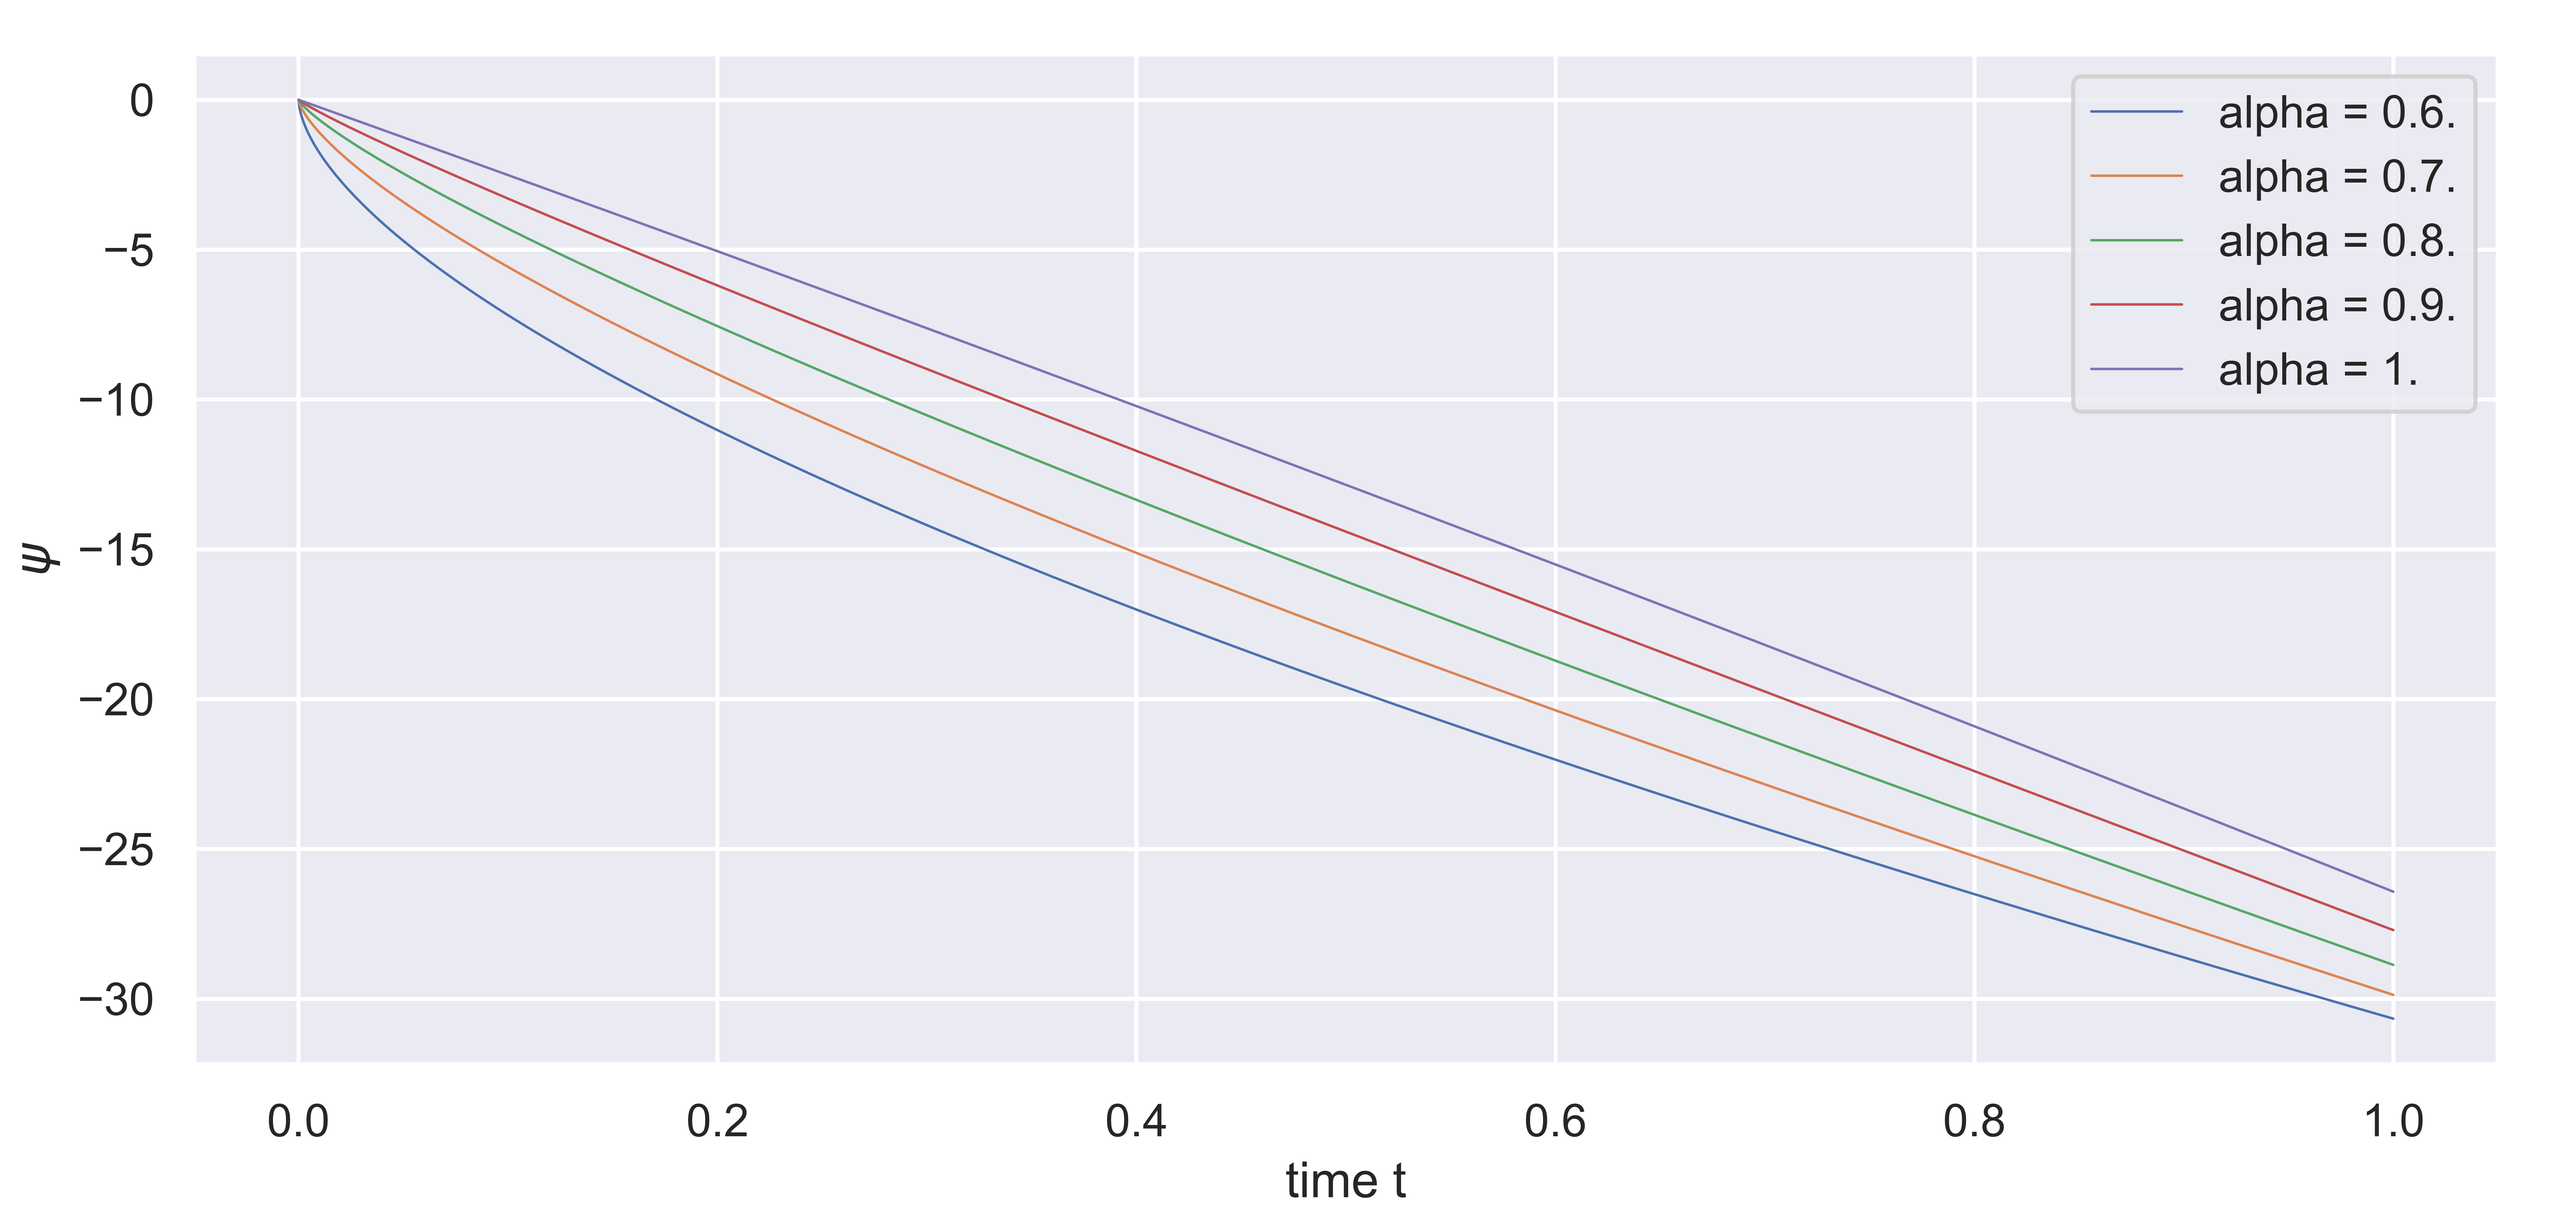
\includegraphics[width = 0.7 \textwidth]{../addition_part/images/numerical_studies/1a.png}
\caption{Plot of $\psi$, which is a key element for the computation of the optimal strategy in \cite{HanWong}. }
\label{fig:1A}
\end{figure}



\begin{figure}
\centering
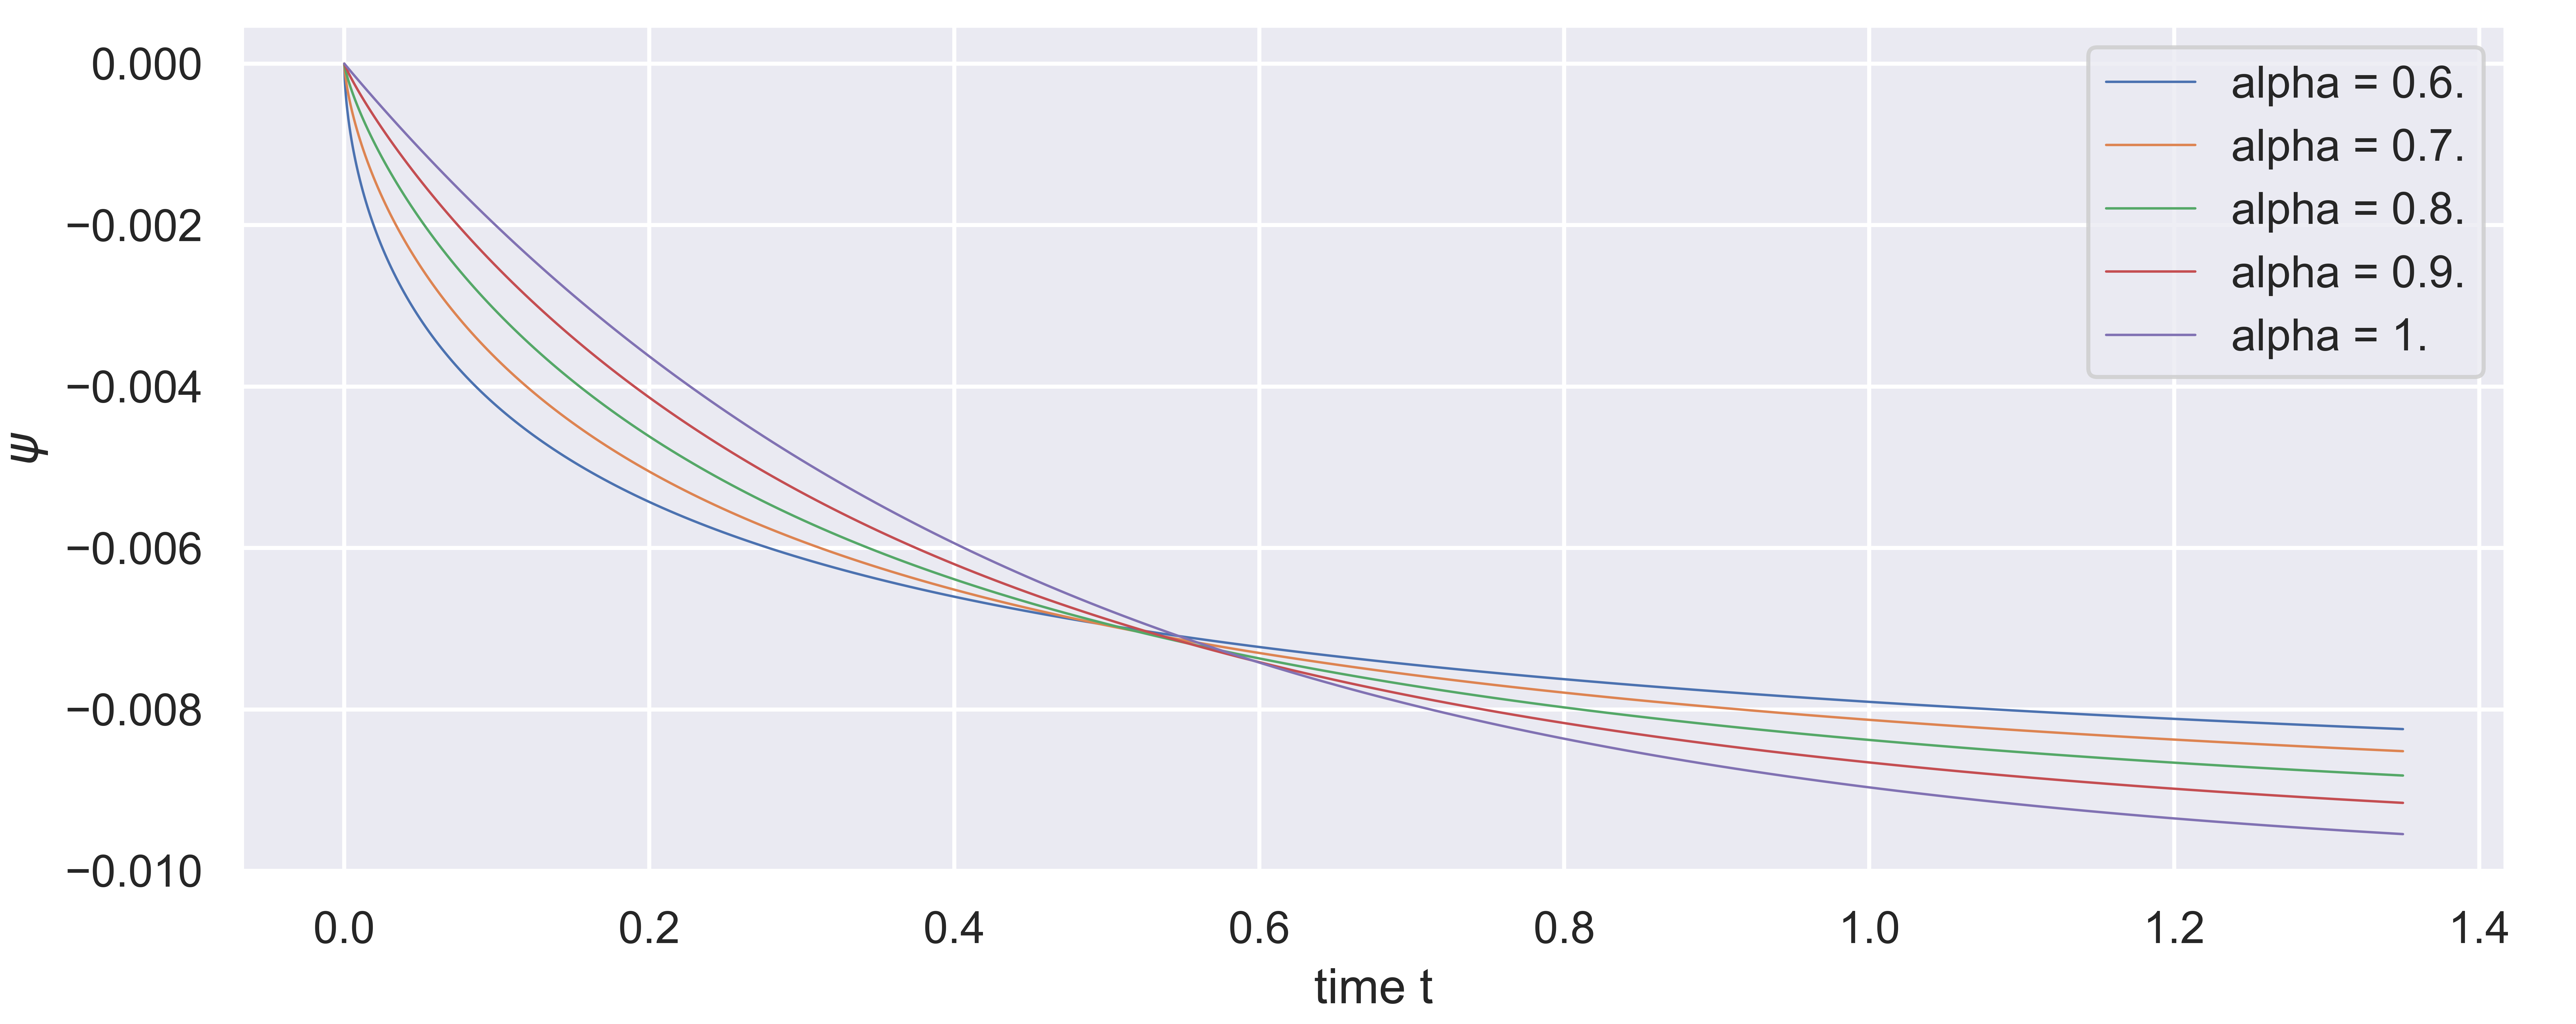
\includegraphics[width = 0.7 \textwidth]{../addition_part/images/numerical_studies/1b.png}
\caption{Plot of $\psi$, under another set of coefficients. }
\label{fig:1B}
\end{figure}









Then, the following step in our research could be computing the optimal strategy, $u^*_t$. To begin with, Han and Wong in \cite{HanWong} fix the volatility and the wealth in the process. As a result, we don't need to simulate anything yet, all the quantities are deterministic. On the other hand, following the definition of $u^*$ (eq. (\ref{eq:optimal_solution})), one sees  that the optimal strategy is heavily dependent on $\psi$ through $A_t$ (eq. (\ref{eq:At})). 
The computations for different alphas can be seen on the fig. \ref{fig:2A} and fig. \ref{fig:2B}, under two sets of parameters given in table \ref{tab:coef2}. Until now, we indeed found the same plots as in \cite{HanWong}, confirming the observations they jotted down in the paper.

\begin{table}
\begin{center}
\begin{tabular}{   m{4.5 cm} | m{4.5 cm} | m{4.5 cm}   } 
\hline
 Parameters & Graph \ref{fig:2A} & Graph \ref{fig:2B} \\ 
\hline
\hline
$\sigma$ & $0.04$ & $3$ \\
\hline
$V_0$ & $0.5$ & $0.5$ \\
\hline
$V_t$ & 0.5 & 0.5 \\
\hline
$x_0$ & $1$ & $1$ \\
\hline
$X_t^*$ & 1 & 1 \\
\hline
$r$ & $0.01$ & $0.01$ \\
\hline
$\rho$ &$ -0.56$ &  $-0.56$\\
\hline
$\theta$  &  $0.15$ &$ 0.15$ \\
\hline
$\kappa$ & $2.25$ & $2.25$ \\
\hline
$\phi$ & $0.15$ &  $0.15$ \\
\hline
T & 1.35 & 1.35 \\
\hline

\end{tabular}
\caption{The two different sets of parameters for $u^*$.}
\label{tab:coef2}
\end{center}
\end{table}



\begin{figure}
\centering
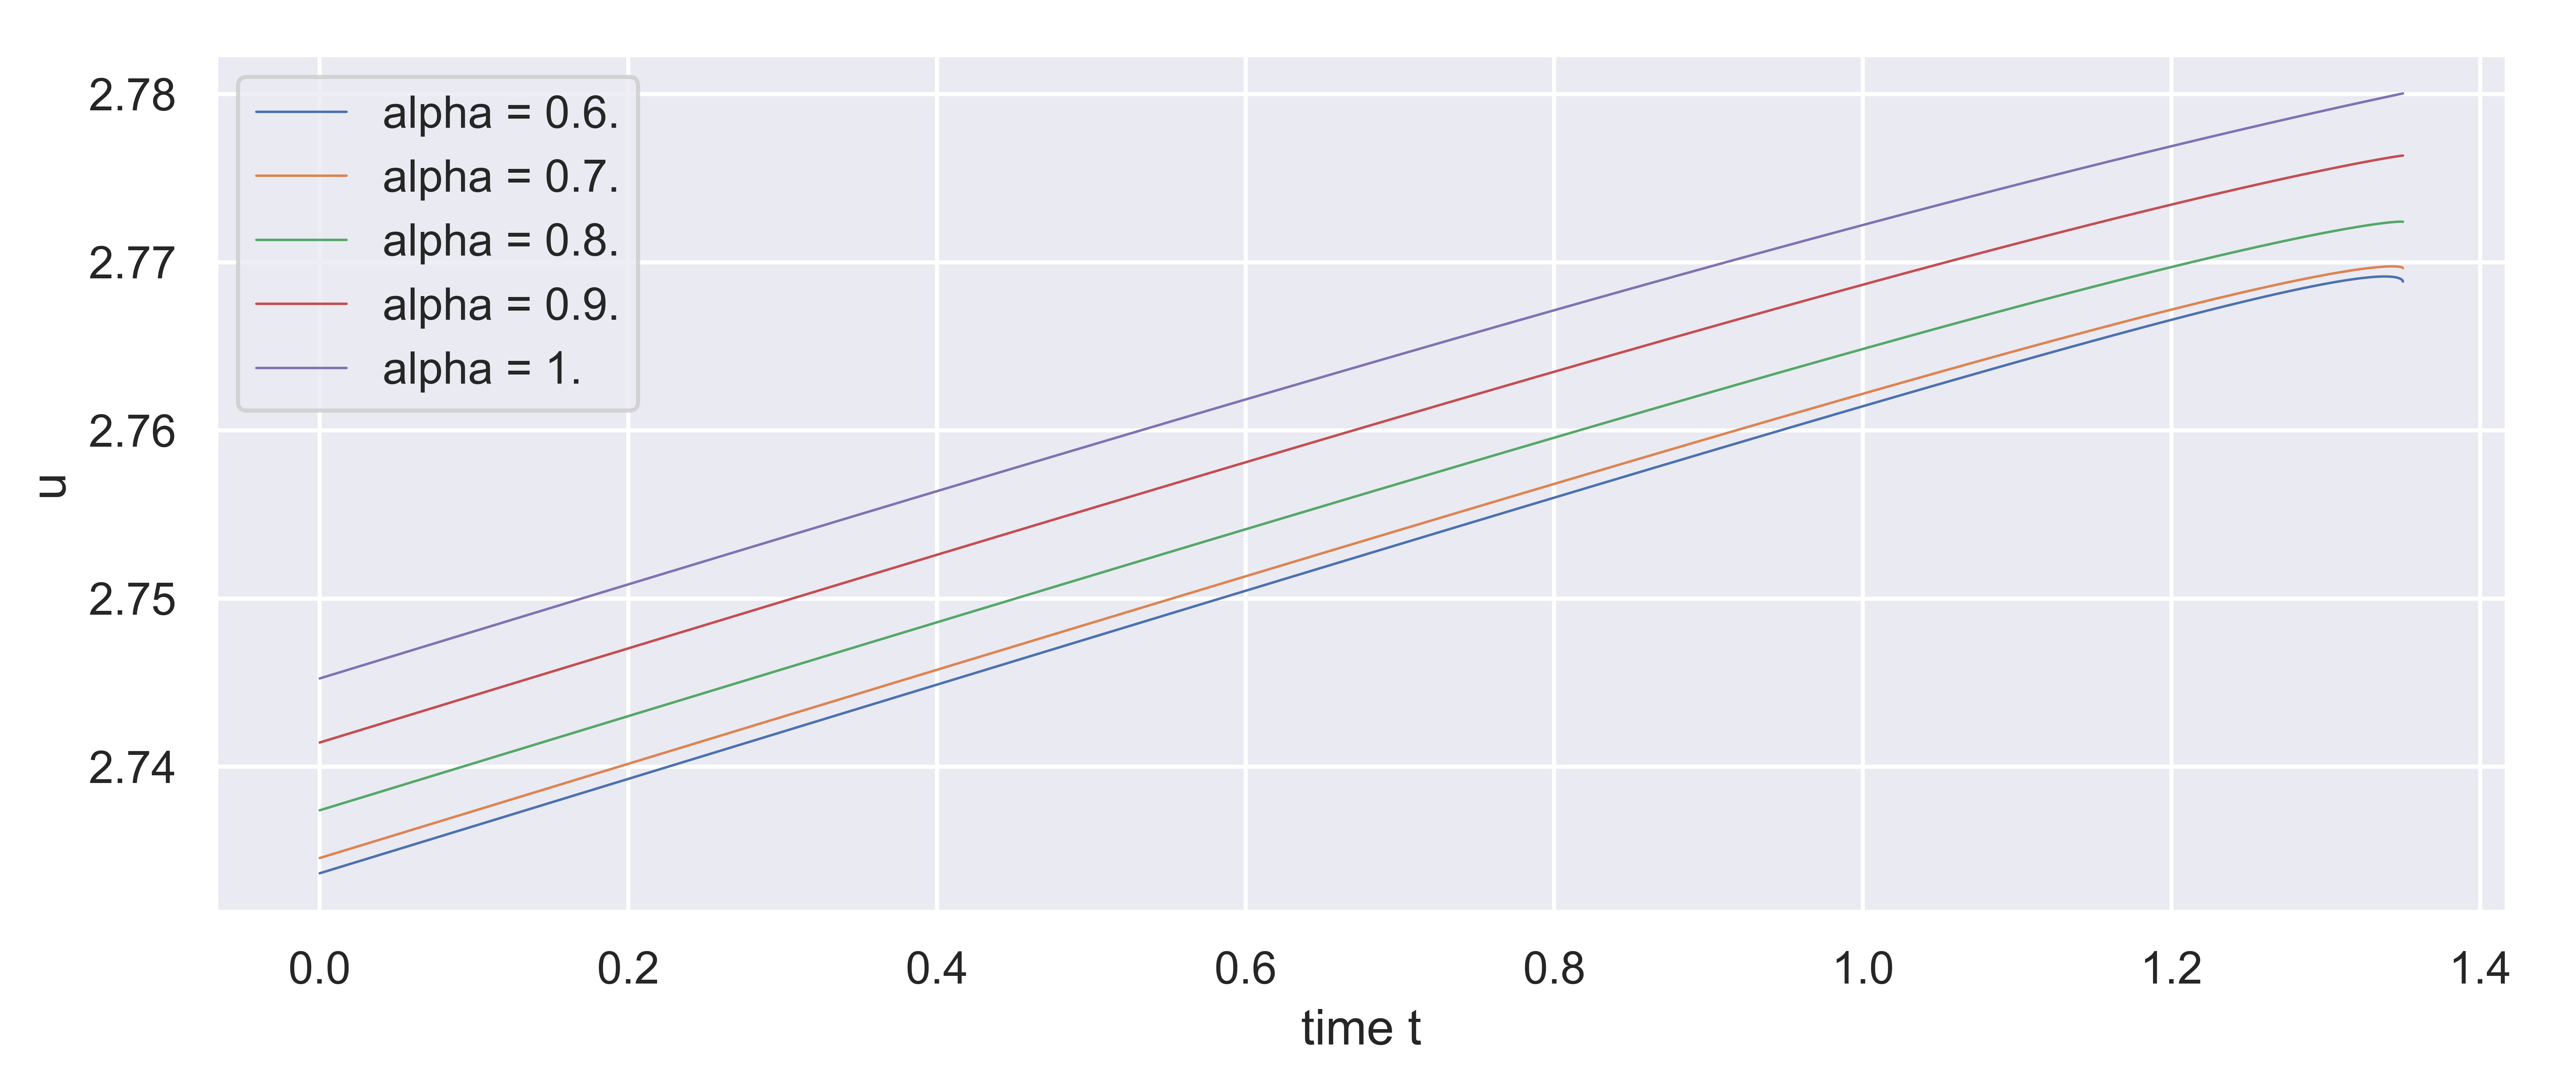
\includegraphics[width = 0.7 \textwidth]{../addition_part/images/numerical_studies/2a.png}
\caption{Optimal strategy, first set of parameters, fixed volatility and wealth.}
\label{fig:2A}
\end{figure}

\begin{figure}
\centering
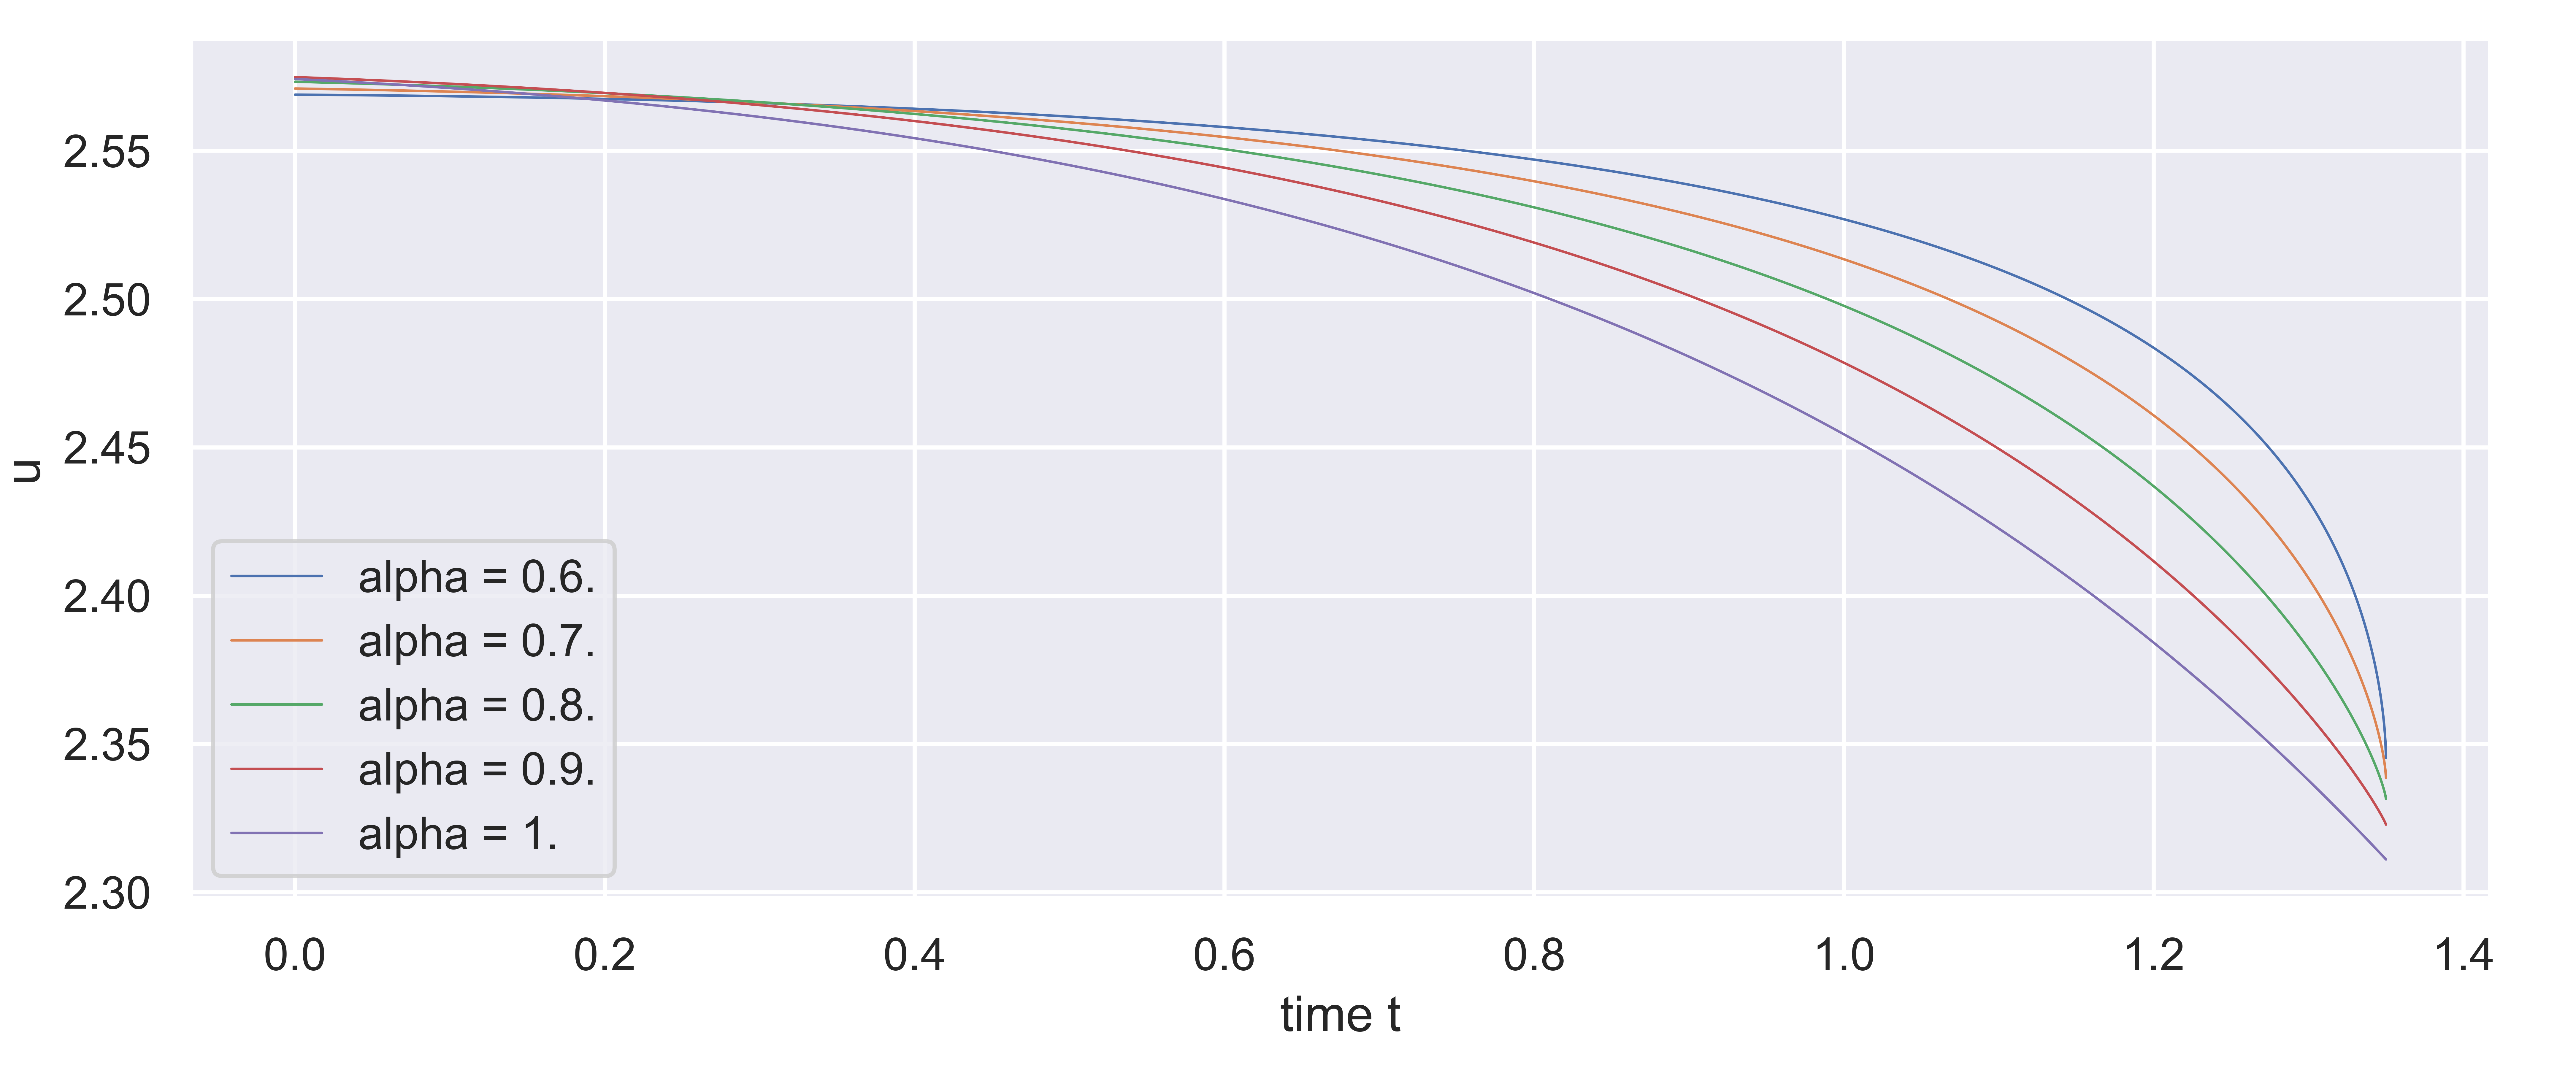
\includegraphics[width = 0.7 \textwidth]{../addition_part/images/numerical_studies/2b.png}
\caption{Optimal strategy, second set of parameters, fixed volatility and wealth.}
\label{fig:2B}
\end{figure}

































\section{Simulating Variance and other stochastic Processes }
\label{processes}

\subsection{Method for simulation}

In order to add some randomness to the model, we need to simulate stochastic processes (i.e. random processes). This is done by integrating random variables into the equations\footnote{In our case, we simulate normal random variables that appear through the Brownian motion of the equations.}.

The easiest case to simulate is the markovian one. Its simplicity comes from the possible conversion between the integral expression and the differential form / flow form. 
An equation that look like this:


$$
d V_t = \kappa  (  \phi - V_t ) dt + \sigma \sqrt{V_t} dB_t 
$$

can be approximated, over a discrete time-grid by this discrete equation:

$$
V_{t+\Delta t} - V_t = \kappa  ( \phi - V_t ) \Delta t + \sigma \sqrt{V_t} \mathcal N ( 0, \Delta t )  
$$

where $\mathcal N ( 0, \Delta t )  $ coins a normal random variable with mean $0$ and variance $\Delta t $. Recall also that 
$$  \mathcal N ( 0, \Delta t )  = \sqrt{ \Delta t } \mathcal N ( 0, 1 )   $$

The good part of this expression is that it does not depend on the discretization of the times since Brownian motion has independent increments. Thus, one can lower the number of points of that expression without affecting the precision of the rest of the computations. 

Here we apply that idea of discretization to our main equations :

\begin{align}
V_{t+\Delta t}  &= V_t + \kappa  ( \phi - V_t ) \Delta t + \sigma \sqrt{V_t} \mathcal M  \\
\mathcal M &= \rho  \left ( \mathcal N_1 ( 0, \Delta t )  + 2 \theta \sqrt{ V_t} \Delta t \right ) +   \sqrt{ 1 - \rho^2 } \mathcal N_2 ( 0, \Delta t ) \\
S_{t+\Delta t} &= S_t + S_t ( r_t + \theta V_t ) \Delta t + S_t \sqrt{V_t} \mathcal N_1 ( 0, \Delta t ) , \quad S_0 > 0 
\end{align}

Please note that if a process can not be expressed as a flow, then one can not simulate the process in such a way. The non-markovian cases we deal with are the rough cases, and other methods are presented in section \ref{rough_heston}.

At this stage, we are able to simulate all the processes from the equations we describe at the beginning of the chapter. However, a problem arises: a Brownian motion can be negative and lead the expression towards negative values, while one still needs to take the square root of the volatility in the dynamics. 

\subsection{How to deal with negative variance ?}

Following the advices from \cite{reflexion}, one is able to deal with negative variance. Since variance is simulated with the help of a Brownian motion, for certain sets of parameters, it reaches zero with positive probability (actually, one condition assures us that the variance will be negative with probability 0, cf. Feller Condition in appendix \ref{feller_condition}). However, the variation process is taken under a square root, making it problematic when the process crosses the x-axis. At the same time, changing the equations by forcing the variance to remain positive may have an impact on the simulation. We want to minimize the latter.

In \cite{reflexion}, Roger Lord, Remmert Koekkoek and Dick van Dijk propose to include three functions in the variance process. The variance becomes:

\begin{align*}
\widetilde{V}(t + \Delta t) &= f_1( \widetilde{V} (t) ) - \kappa \Delta t \cdot \left ( f_2( \widetilde{V}(t) ) - \overline{V} \right ) + \omega  f_3( \widetilde{ V} (t) )^\alpha \Delta W_V(t) \\
V(t+\Delta t ) &= f_3 ( \widetilde{V}(t + \Delta t) ) 
\end{align*}

where $\widetilde{V}$ is a process that might be negative, $ \overline{V}$ the long-term variance.


\begin{table}
\begin{center}
\begin{tabular}{  | m{3 cm} | m{1.5 cm} | m{1.5 cm} | m{1.5 cm} | } 
\hline
Scheme & $f_1$ & $f_2$ & $f_3$  \\ 
\hline
\hline
Absorption & $  x^+ $ & $ x^+ $ & $ x^+ $ \\
\hline
Reflection & $ \abs x $ & $ \abs x $ & $ \abs x $ \\
\hline
Full truncation & $ x $ & $ x^+ $  & $ x^+ $ \\
\hline

\end{tabular}
\caption{Three different schemes, $x^+ = \Max(0,x) $.}
\label{tab:reflections}
\end{center}
\end{table}

The whole discussion of the paper is the attempt to improve the classical "reflection" method used (cf. table \ref{tab:reflections}). We omit the details; they prove in the paper strong convergence of full truncation, so this is the scheme we are going to use for the simulations. For shortness, we haven't written all the proposed schemes and justification. One is invited to take a look at the original paper. Their main concern was to keep the bias induced by the choice of the function to be the smallest.












\subsection{Results of simulations}

The previous sections explained the technical difficulties of simulating stochastic volatility models, when the model is markovian. In the following page, one is able to see the different computations and simulations, gears of the whole mechanism (fig. \ref{fig:dynamics}). I couldn't find the parameters used in \cite{HanWong}, so I used the set of coefficients given by table \ref{tab:coef3}. The plots are not very informative, though they are a proof of the fact that my computations are running. We observe the impact of randomness on the model. One can in particular compare the graph of $u^*$ when no randomness is involved to the new ones. We clearly see how $u*$ is affected by the incorporated Brownian motion. Also, one can notice on the plot of the volatility the effect of negative variance on the process. The full truncation makes the volatility equal to 0 on certain portion of the time.

At this stage, it is also possible to draw the efficient frontier which puts into relation the expected payoff with the risk he has to take. We take eq. (\ref{eq:variance_process}) and compute it for various $\alpha$ and various $c$. The former has an impact on $\psi$, and the latter appears in the expression of the variance.  Then we get the frontier, which shows the impact of the model over the mean-variance portfolio selection. The figure for the efficient frontier is fig. \ref{fig:efficientfrontier}, using the same parameters as in the previous paragraph. We observe that there is a (negative) linear relationship between $\alpha$ and the payoff, which indicates that a rougher model forecasts more payoff in average for a given level of risk. Also, one can observe the classical relationship between the payoff and the variance, for $\alpha = 1$.



\begin{figure}
\centering


\subfloat{{
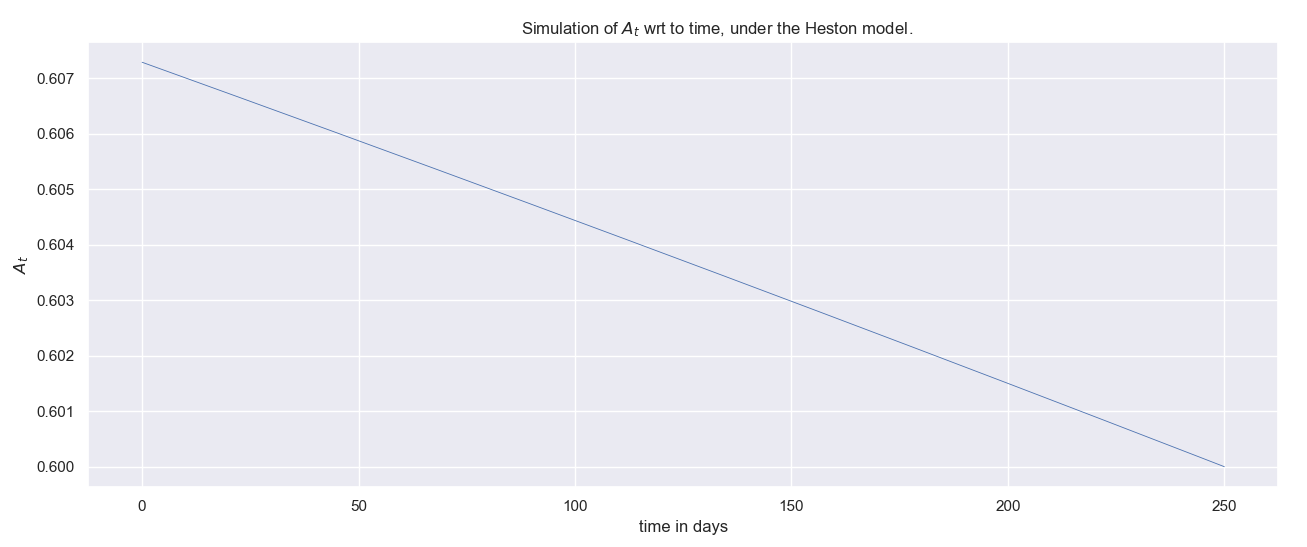
\includegraphics[width = 0.48 \textwidth]{../addition_part/images/numerical_studies/3A_t.png}
}}
\subfloat{{
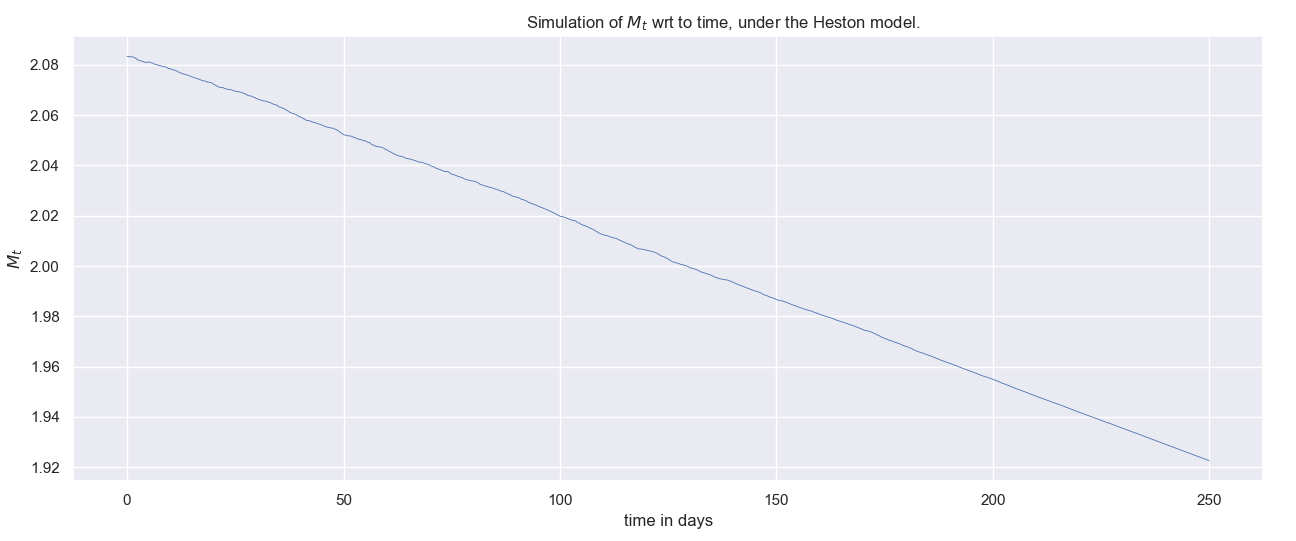
\includegraphics[width = 0.48 \textwidth]{../addition_part/images/numerical_studies/3M_t.png}
}}\\
\subfloat{{
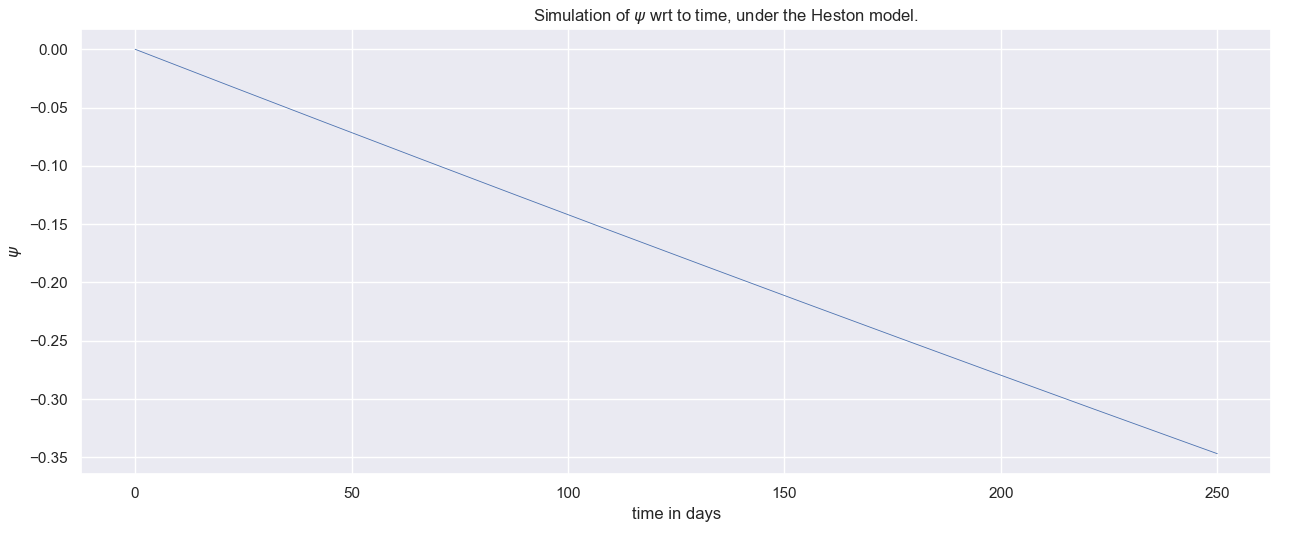
\includegraphics[width = 0.48 \textwidth]{../addition_part/images/numerical_studies/3psi.png}
}} 
\subfloat{{
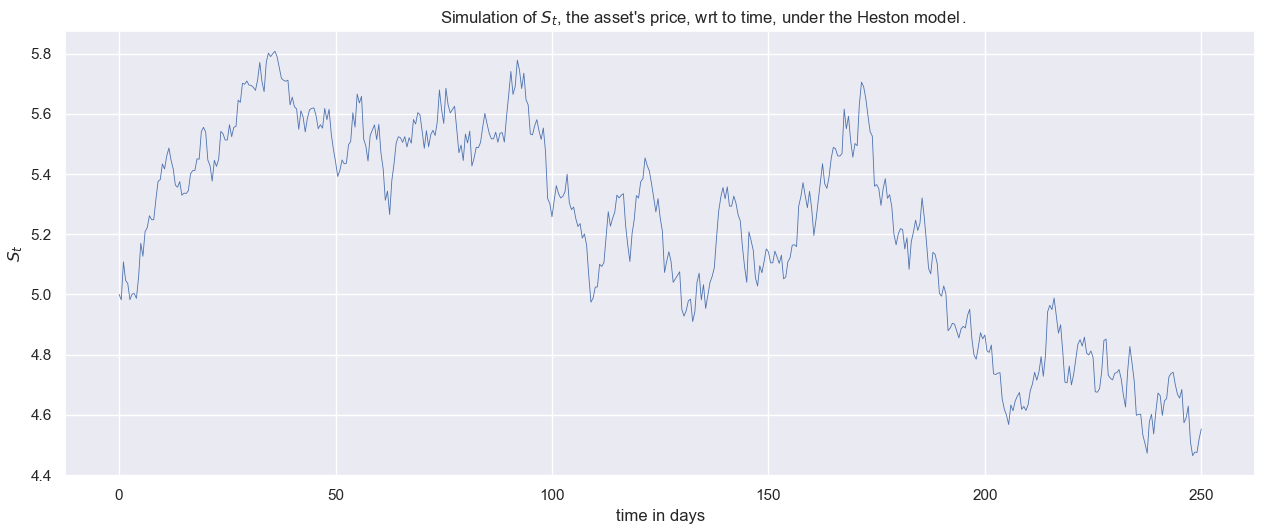
\includegraphics[width = 0.48 \textwidth]{../addition_part/images/numerical_studies/3S_t.png}
}}\\
\subfloat{{
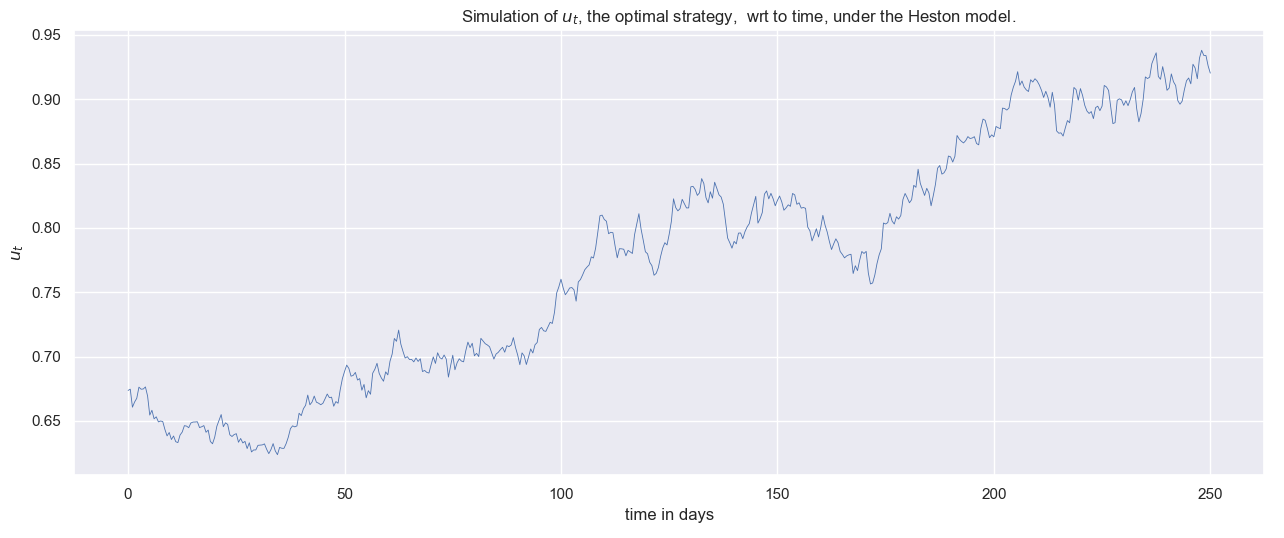
\includegraphics[width = 0.48 \textwidth]{../addition_part/images/numerical_studies/3u_t.png}
}} 
\subfloat{{
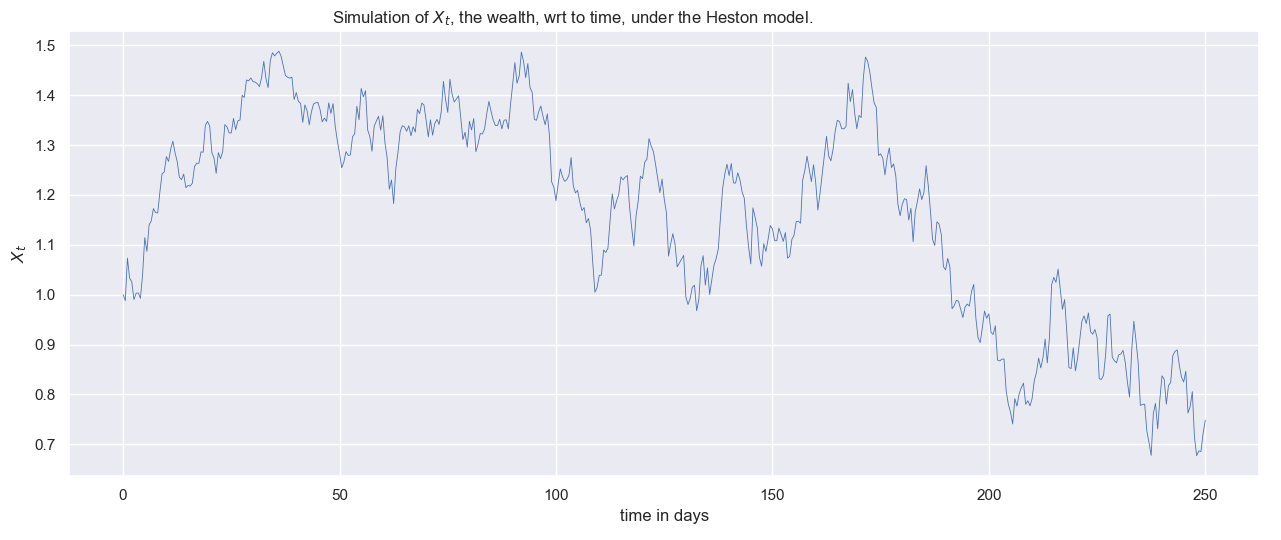
\includegraphics[width = 0.48 \textwidth]{../addition_part/images/numerical_studies/3X_t.png}
}}\\
\subfloat{{
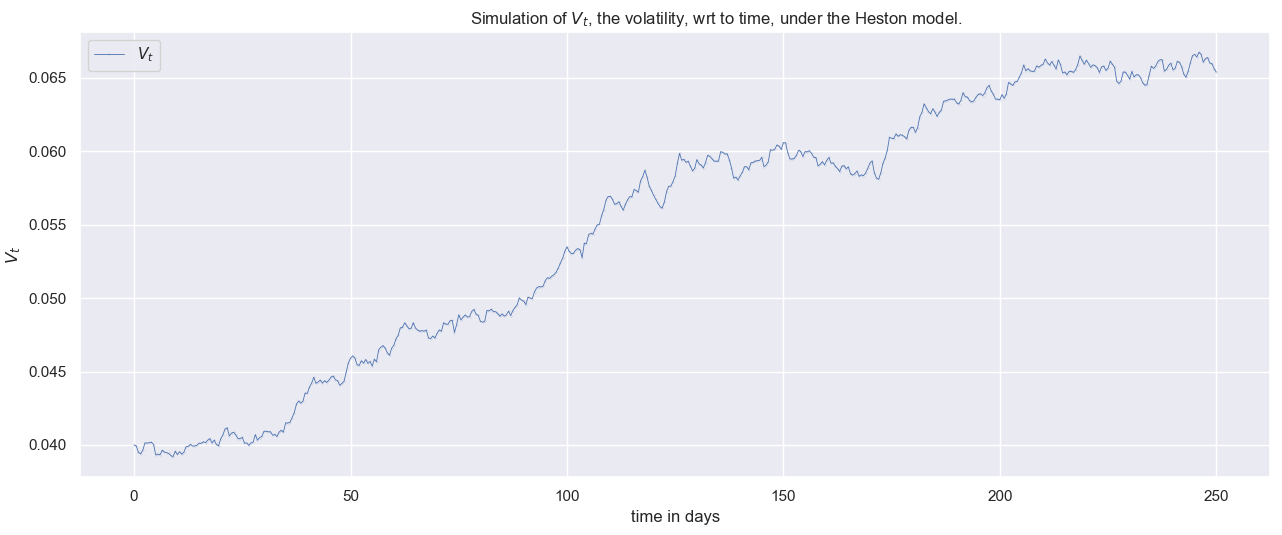
\includegraphics[width =  0.5 \textwidth]{../addition_part/images/numerical_studies/3V_t.png}
}} 

\caption{Dynamics of the different processes and strategies. Respectively, from left to right, top to bottom, $A_t$, $M_t$, $\psi$, $S_t$, $u_t$, $X_t$, $V_t$.}
\label{fig:dynamics}
\end{figure}









\begin{table}
\begin{center}
\begin{tabular}{   m{4.5 cm} | m{4.5 cm}   } 
\hline
 Parameters & Plots  \ref{fig:dynamics} and \ref{fig:efficientfrontier}  \\ 
\hline
\hline
$\sigma$ & 0.03  \\
\hline
$V_0$ &  0.04 \\
\hline
$x_0$ &  1 \\
\hline
$S_0$ & 1 \\
\hline
$r$ & 0.03 \\
\hline
$\rho$ & -0.7\\
\hline
$\theta$  & 0.6  \\
\hline
$\kappa$ & 0.1 \\
\hline
$\phi$ & 0.3  \\
\hline
T & 1 \\
\hline
\end{tabular}
\caption{Set of parameters for simulations of the processes and of the efficient frontier.}
\label{tab:coef3}
\end{center}
\end{table}







\begin{figure}
\centering
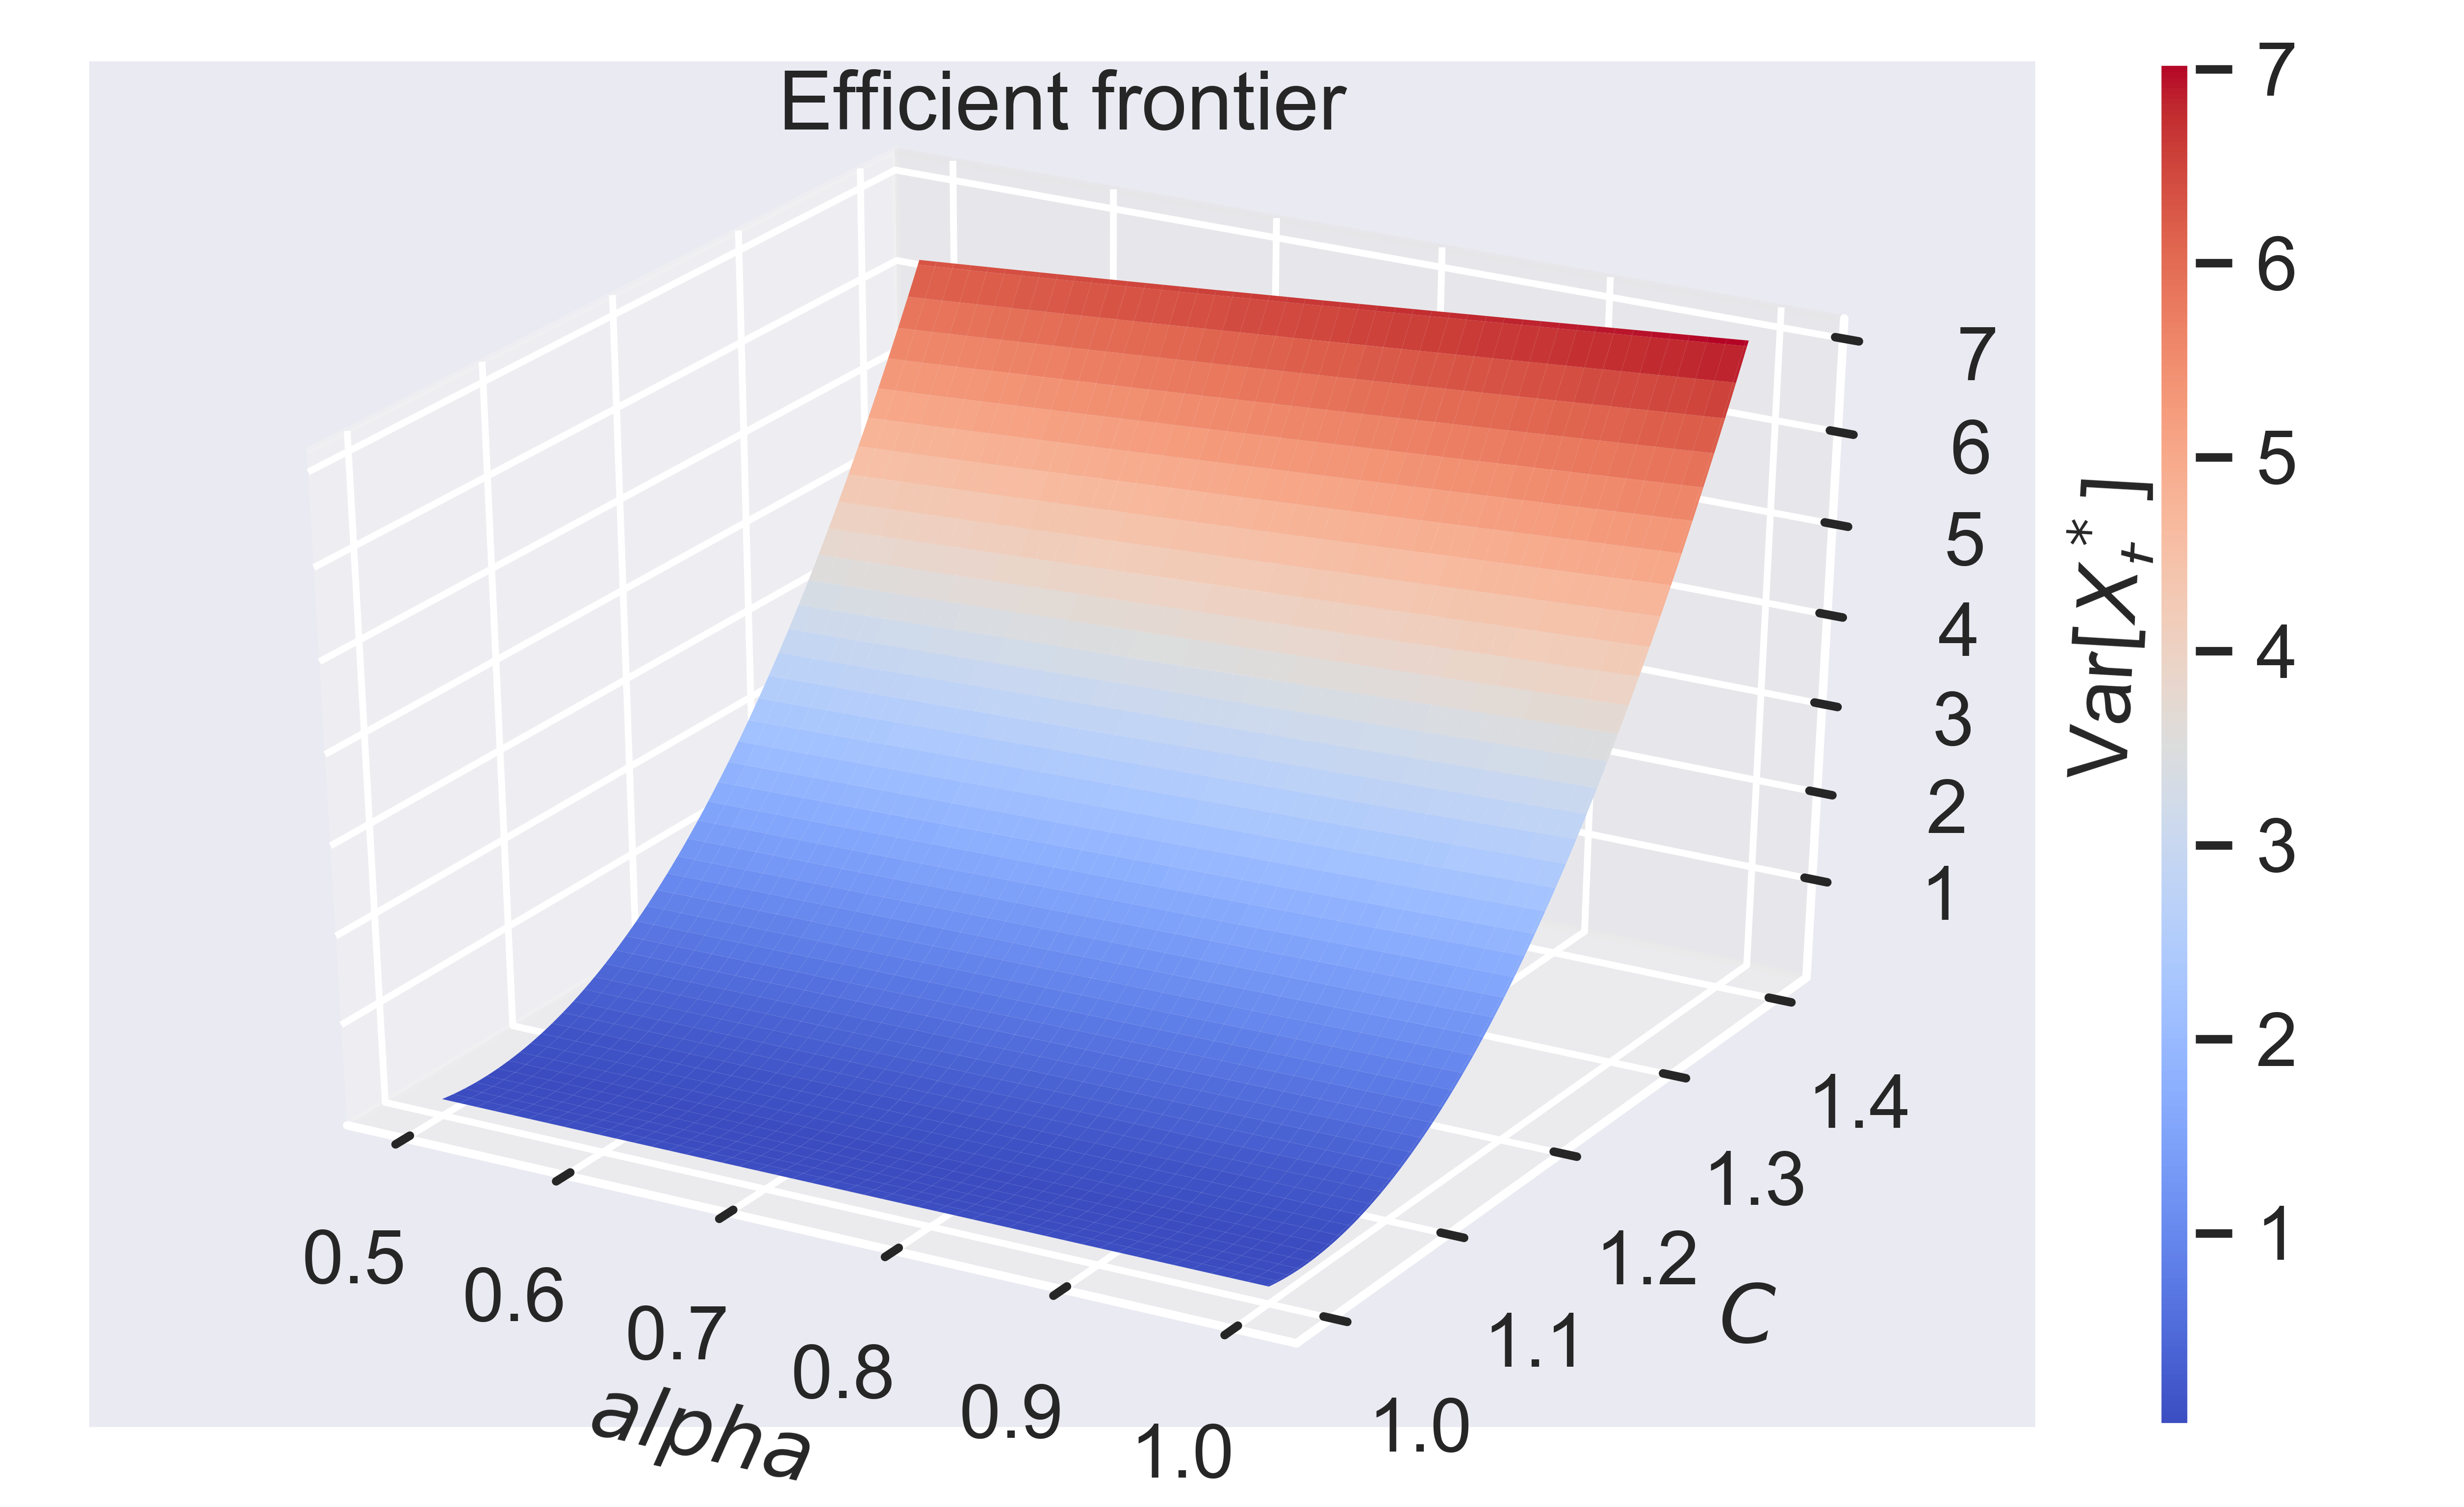
\includegraphics[width = 0.5 \textwidth]{../addition_part/images/numerical_studies/efficient_frontier.png}
\caption{Efficient frontier where one see the influence of $\alpha$ and the choice of the target wealth upon the variance of the portfolio.}
\label{fig:efficientfrontier}
\end{figure}














\section{Rougher Path for Heston }
\label{rough_heston}
As mentioned in \cite{HanWong}, markets are better described by processes that include roughness, or in other words some memory. We describe here two ways to simulate a rougher path. That way, we will be able to simulate the expectation of the wealth as they did in the paper by MonteCarlo method, and compare that indeed, a rougher model leads to a solution closer to the true value.

\subsection{Lifted Heston}

In the paper \cite{lifted}, an attempt to generate rougher path with the help of non-rough path is proposed. Abi Jaber's idea is to use a Heston model with $n$ multi-factors, sharing the same Brownian motion but mean reverting at different speeds. The advantage of the lifted Heston is sharing the best properties of roughness and classic Heston : it is at the same time markovian, a semimartingale, allows a characteristic function and is computed faster than rough Heston.

In more detail, the advantages of that method are, as written in the paper:

\begin{itemize}
\item reproduces the same volatility surface as the rough Heston model for maturities ranging from one week to two years,
\item mimics the explosion of the at-the-money skew for short maturities,
\item calibrates twenty times faster than its rough counterpart,
\item is easier to simulate than the rough model.
\end{itemize}

First, recall the equations of the process, under $\alpha = 1$:

\begin{align*}
dV_t &= ( \kappa \phi - \lambda V_t ) dt + \sigma \sqrt{V_t} d \widetilde{B_t}   \\
d \widetilde{B_s } &:= \rho d [ W_{1,s} + 2 \theta \int_0^s \sqrt{ V_u } du ] + \sqrt{ 1 - \rho^2 } d W_{2,s}   \\
d S_t &= S_t ( r_t + \theta V_t ) dt + S_t \sqrt{V_t} d W_{1,t}, \quad S_0 > 0 
\end{align*}

Then, following the method proposed by Abi Jaber in the paper, and adjusting it to take into account that in our case, the risk premium,  $\theta \neq 0$, we then get the following process. The notations for the processes are consistent with the ones from \cite{lifted}, and the constants were adapted to our previous notations:

\begin{align}
d S_t^n &= S_t^n ( r_t + \theta V_t^n ) dt + S_t^n \sqrt{V_t^n} d W_{1,t}, \quad S_0 > 0  \\
dU_t^{n,i} &= \left ( - x_i^n U_t^{n,i} - \lambda V_t^n \right ) dt + \sigma \sqrt{V_t^n}  d \widetilde{B_t}  \label{eq:lifted_1}  \\
d \widetilde{B_s } &:= \rho d [ W_{1,s} + 2 \theta \int_0^s \sqrt{ V_u } du ] + \sqrt{ 1 - \rho^2 } d W_{2,s}   \\
V_t^n &= g_0^n (t) + \sum^n_1 c_i^n U_t^{n,i} \label{eq:lifted_2} \\
g_0^n  \colon t &\to V_0 + \frac{ \kappa \phi} { \lambda } \sum_1^n c_i^n \int_0^t e^{-x_i^n (t-s) } ds \label{eq:lifted_error}
\end{align}

where the $r_i^n, x_i^n, c_i^n$ are defined in the paper p.6, where the $x_i$ and the $c_i$ are functions of $r_i$.

\begin{remarque}
It is written in the paper that one can modify the coefficients $r_i^n$ in order to increase roughness.
\end{remarque}

Actually, I'd like to correct the last equation as it seems to me that there is a typo. I think it should be:

$$ 
g_0^n  \colon t \to V_0 + \kappa \phi \sum_1^n c_i^n \int_0^t e^{-x_i^n (t-s) } ds
$$

The reason why I think it is the case, is because the model doesn't reduce to the classical Heston. As mentioned in the paper, if one takes 
$$ n = 1, \qquad x_i \equiv 0, \qquad c_i \equiv 1 $$

the model shall reduce to the classical Heston. However, one notices that under taking the original equations (\ref{eq:lifted_error}), the variance converges, when $T$ increases, to $\frac {\phi } {\kappa}$ instead of converging to $\phi$ as it should. This can be verified mathematically that under the previously mentioned assumption, the variance process does not come back to the classical case: 


\begin{align*}
V_t^n &= g_0^n (t) + \sum^n_1 c_i^n U_t^{n,i} \\
&= V_0 + \frac{ \kappa \phi} { \lambda } \sum_1^n c_i^n \int_0^t e^{-x_i^n (t-s) } ds 
+ \sum^n_1 c_i^n U_t^{n,i} \\
&= V_0 + \frac{ \kappa \phi} { \lambda } t
+ U_t^{n,1} \\
&= V_0 + \frac{ \kappa \phi} { \lambda } t + U_t^{n,1}
\end{align*}
then 
\begin{align*}
dV_t^n &= \frac{ \kappa \phi} { \lambda } dt + dU_t^{n,1} \\
&=  \frac{ \kappa \phi} { \lambda } dt - \lambda V_t^n dt + \sigma \sqrt{V_t^n}  d \widetilde{B_t} \\
&= ( \frac{ \kappa \phi} { \lambda } - \lambda V_t ) dt + \sigma \sqrt{V_t} d \widetilde{B_t}
\end{align*}

On the other hand, if one takes the other expression of $g_0$, where $\kappa \phi $ substitutes $\frac{ \kappa \phi} { \lambda }$ the results agree with the original variance flow form. I am thus going to stick with that expression of $g_0$ for the simulations.

\begin{figure}
\centering
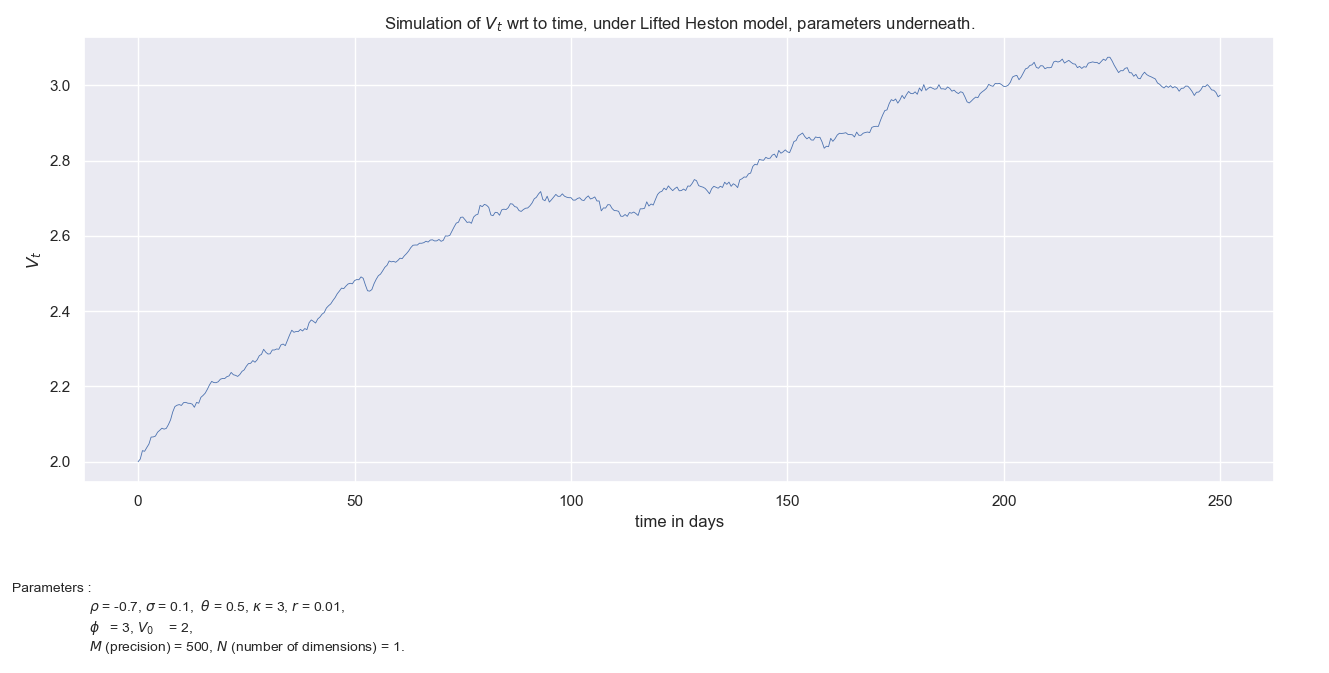
\includegraphics[width = 0.8 \textwidth]{../addition_part/images/numerical_studies/Lifted_V_t.png}
\caption{Lifted Heston as proposed by Abi Jaber in \cite{lifted}, degenerated case into normal Heston.}
\label{fig:liftedV}
\end{figure}

\begin{figure}
\centering
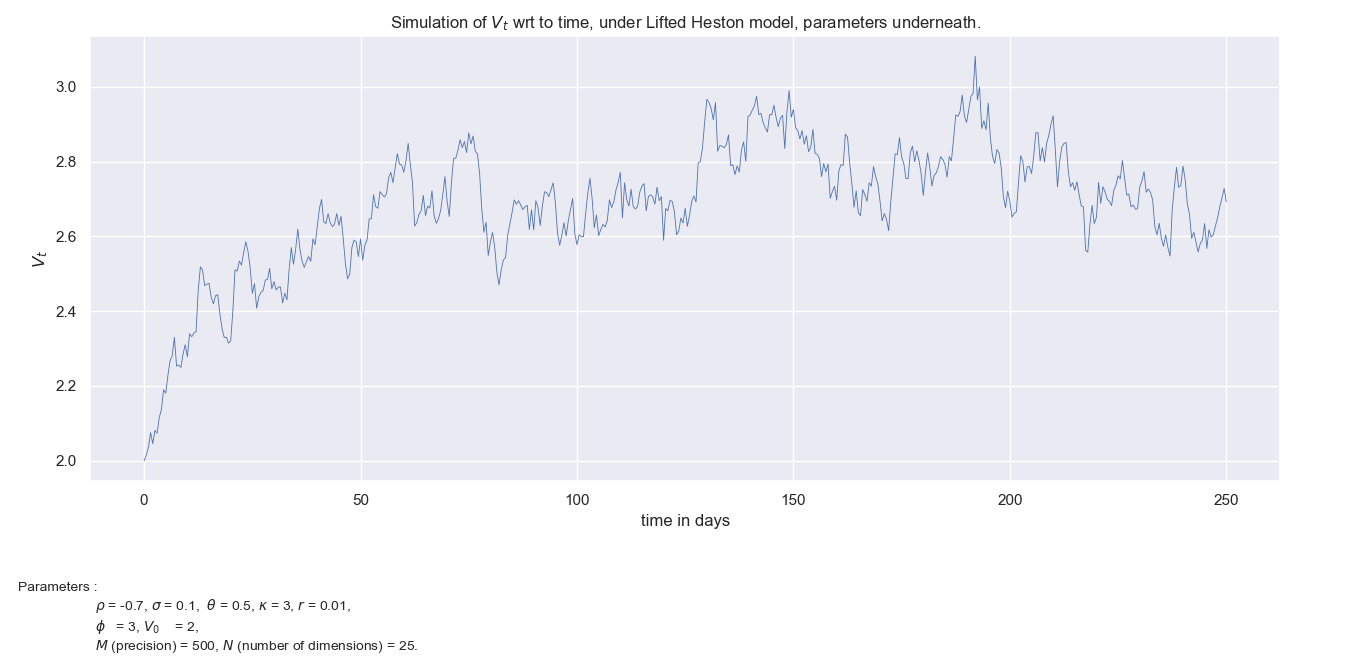
\includegraphics[width = 0.8 \textwidth]{../addition_part/images/numerical_studies/Lifted_V_t_2.png}
\caption{Lifted Heston as proposed by Abi Jaber in \cite{lifted}, 25 dimensions.}
\label{fig:liftedV_2}
\end{figure}



So at the end of the day, in order to compute the lifted Heston, one first computes $g_0^n$, then simulates $\forall i \colon U_t^i$ and $V^n$ incrementally. 

Additionally, aware of the difficulty of dealing with negative variance, I used the same scheme as for normal Heston, in other words the full truncation. The expression of the volatility using the four functions $f_i$ looks like this. Plugged in eq. (\ref{eq:lifted_1}) and in eq. (\ref{eq:lifted_2}):

\begin{align*}
dU_t^{n,i} &= \left ( - x_i^n U_t^{n,i} - \lambda f_2(V_t^n) \right ) dt + \sigma \sqrt{ f_3(V_t^n) }  d \widetilde{B_t} \\
d \widetilde{B_s } &= \rho d [ W_{1,s} + 2 \theta \int_0^s \sqrt{ f_2(V_u) } du ] + \sqrt{ 1 - \rho^2 } d W_{2,s} \\
V_t^n &= f_3 \left ( g_0^n (t) + \sum^n_1 c_i^n U_t^{n,i} \right )
\end{align*}

Also, one can evaluate by hand, before computation, the integral inside $g_0$ :

$$ \int_0^t e^{-x_i^n (t-s) } ds  
= \int_0^t e^{-x_i^n s } ds 
= \begin{cases} 
t, & \mbox{ if } x_i^n = 0 
\\ 
\frac {1} { x_i^n } ( 1 - e^{-x_i^n t } )  , & \mbox{ if } x_i^n \neq 0   
\end{cases}
$$ 

Here are two plots; the first one corresponds to the lifted Heston degenerating to the normal Heston, fig. \ref{fig:liftedV} ; the second plot is the rough Heston generated by 25 dimensional lifted Heston, fig. \ref{fig:liftedV_2}. The first plot shows a variance that is quite similar to the original one (from \ref{fig:dynamics}), and converges to the long term expected value\footnote{$\phi$}. On the other hand, increasing the number of dimensions obviously increases the roughness of the volatility. We can't really know if the volatility is exactly the way it is supposed to be. However, a good way to test that is checking whether the optimal solution from \cite{HanWong} gives an increase in wealth in expectation.



\subsection{Rough Heston}
\label{rough}

On the other hand, one can simulate directly the Rough Heston volatility process. Pr. Jacquier shared with me one of his own paper \cite{ROUGH_HESTON}.

In there, a scheme to generate directly rough Heston paths is described. 

In the paper, it is proposed to simulate the following dynamic, where we kept the same notations: 

$$
V_t = V_0 + \int_0^t K(t-s) [ \kappa ( \theta - V_s ) ds + \xi \sqrt{ V_s } d B_s ]
$$

We translate some of the equations mentioned in the paper in order to be consistent with our previous notations, Han Wong's paper notation.
The modification we do are we add the drift (due to the risk premium $\theta$) to the first Brownian motion $dBs$, as well as adapting the notations for the constants. 

Then, $V_t$ can be rewritten as:

$$
V_t = V_0 + \int_0^t K(t-s) [ \kappa \theta - \lambda V_s  ds + 2 \rho \sigma \theta V_s ds + \xi \sqrt{ V_s } d B_s ]
$$


In order to simulate the volatility process, a regular discrete time-grid is introduced. Then, one computes $V_{t_i}$ for all those time points incrementally. Since the process is no more markovian, $V_{t_i}$ depends on $ \forall j < i, V_{t_j}$. 

Then, we slice the integrals, and we freeze the volatility of every integral on each subinterval to its left-point value. 
Also, we isolate in the last part of the expression the singularity induced by the kernel (recall that the kernel introduces the quantity $t^{\alpha - 1} $ which for $\alpha < 1$ diverges toward infinity in 0). 
Then, using some advanced mathematical tools, they succeed in finding a good approximation to the values of the stochastic integrals. 

In the following, we denote by $t_i$ any element from the grid of times, and we use the index $i$ inside the sums.


\begin{align}
V_{t_i} &= V_0 + \int_0^{t_{i}} K(t_i-s) [ \kappa \phi - \lambda V_s  ds + 2 \rho \sigma \theta V_s ds + \sigma \sqrt{ V_s } d B_s ]    \notag   \\
&= V_0 + \sum_{j=0}^{i-1} [ \kappa \phi + (-\lambda + 2 \rho \sigma \theta ) V_j ] A_{j,i}  \notag \\
& \quad + \sum_{j=0}^{i-2} \sigma \sqrt{ V_j } \int_{t_j}^{t_{j+1} } K( t_i - s ) dB_s + \sigma \sqrt{ V_{i-1} } \int^{t_i}_{t_{i-1}} K( t_i - s ) dB_s  \notag \\
&= V_0 + \sum_{j=0}^{i-1} [ \kappa \phi + (-\lambda + 2 \rho \sigma \theta ) V_j ] A_{j,i} 
+ \sum_{k=2}^{i} \sigma \sqrt{ V_{i-k} } \int_{t_j}^{t_{j+1} } K( \frac{b_k^*}{n} ) \overline{B}_{i-k} + \sigma \sqrt{ V_{i-1} } \tilde{B }_{i-1}  \label{eq:rough_heston_final_form}
\end{align}

where $$ A_{j,i} = \frac 1 {\Gamma ( \alpha +1 ) } [ ( t_i - t_j )^{\alpha} -  ( t_i - t_{j+1} )^{\alpha} ]$$
in the case of a power law kernel: $ K(t) = \frac{t^{\alpha - 1} }{\Gamma ( \alpha ) } $ as long as $\alpha \in ]0.5,1.5[$;

$( \overline{B}_{i-k},\tilde{B}_{i-1}) $ forms a two-dimensional Gaussian vector, whose covariance matrix $\Sigma$ is given by

$$ \Sigma_{11} = \Delta, \qquad \Sigma_{12} = \Sigma_{21} = \frac 1 {\Gamma ( \alpha + 1 ) } \Delta^{\alpha}, \qquad \Sigma_{22} = \frac{1}{ \Gamma (\alpha ) ( 2 \alpha - 1 ) }  \Delta^{2 \alpha - 1} $$
which can be obtained with a Cholesky decomposition,

finally, $$b_k^* := \left ( \frac{k^{ \alpha} (k-1)^{ \alpha} }{    \alpha }  \right )^{\frac{1}{\alpha - 1} } $$







There is no proof that using reflection scheme or full truncation would lead to any kind of convergence. That would be something to verify. Here is how we apply full truncation to the volatility process. By coming back to eq. (\ref{eq:rough_heston_final_form}):

\begin{align*}
\widetilde{V}_t &= V_0 
+ \sum_{j=0}^{i-1} [ \kappa \phi + (-\lambda + 2 \rho \sigma \theta ) f_2(\widetilde{V}_j) ] A_{j,i}  \\
& \qquad \qquad + \sum_{k=2}^{i} \sigma \sqrt{ f_3(\widetilde{V}_{i-k}) } \int_{t_j}^{t_{j+1} } K( \frac{b_k^*}{n} ) \overline{B}_{i-k} 
+ \sigma \sqrt{ f_3(\widetilde{V}_{i-1}) } \tilde{B }_{i-1},  \\
 V_t &= f_3( \widetilde{V_t} )
\end{align*} 

\begin{remarque}
We have defined the covariance matrix between $( \overline{B}_{i-k},\tilde{B}_{i-1}) $. Hence, it is easy to derive the covariance matrix between the three processes (two processes for the volatility, and one, with correlation $\rho$ with them, used for simulating the path of the asset's price) is given by: 
$$
\begin{pmatrix} 
\Sigma_{11} & \Sigma_{12}  & \rho / n
\\ 
\Sigma_{21} & \Sigma_{22} &  \rho \Sigma_{12}
\\
\rho / n & \rho \Sigma_{12} & 1/n \end{pmatrix}
$$
\end{remarque}

\begin{remarque}
Also, as a conclusion for the paper of Pr. Jacquier, one should remember that even though we use in our case a power-law kernel, the kernel can be changed and it will impact some of the constants. Also, for more advanced kernels, it is possible to use the Toeplitz nature of the matrix $(A_{j,i})_{ j \in \{1 \cdots n \} , i \in \{1 \cdots n \} } $ in order to reduce the computational cost.
\end{remarque}


\textbf{Commentary about $\alpha$'s choice:}
\begin{itemize}
\item  It is possible to set $\alpha > 1.5$. In that case, by what we wrote in chapter 1 about Hölder Continuity of the model, and by using the fact that any function $h$-Hölder with $h> 1$ is constant, we expect the variance process to be flat. Empirically, it is almost flat, modulo some numerical errors.

\item Setting $\alpha = 1$ (resp. $\alpha = 0.5$) is not possible as the function diverges at this value, but one can input a value very close to 1 (resp. $0.5$) and the model degenerates back to the classical Heston.

\item The simulation doesn't work for $\alpha \in [1;1.5]$. The covariance matrix is not positive definite.
\end{itemize}

\subsection{Final Results}

The final results of that section are maybe also the most important ones. At this stage, we are able to simulate the normal and rough Heston. The last plots we needed for completeness  of the paper \cite{HanWong} are the boostrap of the wealth. If everything works correctly, we expect the wealth to grow and reach (almost) the targeted wealth. Also, the whole purpose of the paper \cite{HanWong} was to prove that under a rougher model of the market, one reaches the targeted wealth with less volatility. This is something great as it is the crucial target of mean-variance portfolio theory. 

We saw that indeed, rougher Heston reduces the variance of a strategy (cf. fig. \ref{fig:efficientfrontier}) for a fixed expected payoff. Since the optimal strategy fixes the variance allowed, and reaches the best profit\footnote{In average.}, one expects that the final wealth will be higher for rougher models.

We plot in the following figures (fig. \ref{fig:bootstrap}, fig. \ref{fig:bootstraplifted}, fig. \ref{fig:bootstraprough}) the comparison between the optimal strategy, the volatility and the wealth, under the normal, lifted and rough Heston. We use the parameters from table \ref{tab:bootstrap}. First notice that the volatility appears rougher for the lifted version and rough version than the normal version, which is something we expected.

The black dotted line on the graph of the wealth is the targeted  wealth at horizon. We observe that though the targeted wealth is not perfectly reached, the wealth under rougher models\footnote{One can compare profit from the rough model simulated with the paper of Mr. Jacquier and Mr. Jaber.} is higher\footnote{and closer to the target.} than from classical Heston, which is what we expected. I simulated the same plots for another set of parameters, for checking whether the results were pure luck. They are visible on fig. \ref{fig:bootstrap}, fig. \ref{fig:bootstraplifted}, fig. \ref{fig:bootstraprough}. The same phenomenon appears, even though it is less blatant. The rougher models offer a payoff constantly higher than their classical counterpart.  The two main results are that rougher models earn more money at equal level of risk, and are closer to the targeted wealth at the horizon.

We have checked that \cite{HanWong}'s results are indeed correct.

\begin{table}
\begin{center}
\begin{tabular}{   m{4.5 cm} | m{4.5 cm}  | m{4.5 cm}  } 
\hline
 Parameters & Bootstraps 1 & Bootstraps 2 \\ 
\hline
\hline
$\sigma$ & 0.1 &  0.03 \\
\hline
$V_0$ &  0.26 &  0.26\\
\hline
$x_0$ &  1 & 1 \\
\hline
$S_0$ &  1 & 1 \\
\hline
$r$ & 0.01 & 0.01 \\
\hline
$\rho$ & -0.7 & -0.7 \\
\hline
$\theta$  & 0.15  &  0.2\\
\hline
$\kappa$ & 1.5 & 1.5  \\
\hline
$\phi$ & 0.3  & 0.5 \\
\hline
$T$ & 1 & 1 \\
\hline
$C$ & 1.116  &  1.116 \\
\hline
$\alpha$ & 0.6 & 0.6 \\
\hline
nb. of simul. & 10 000 & 20 000 \\
\hline
\end{tabular}
\caption{Set of parameters for bootstrap.}
\label{tab:bootstrap}
\end{center}
\end{table}



\begin{figure}[h]
\centering
\subfloat{{
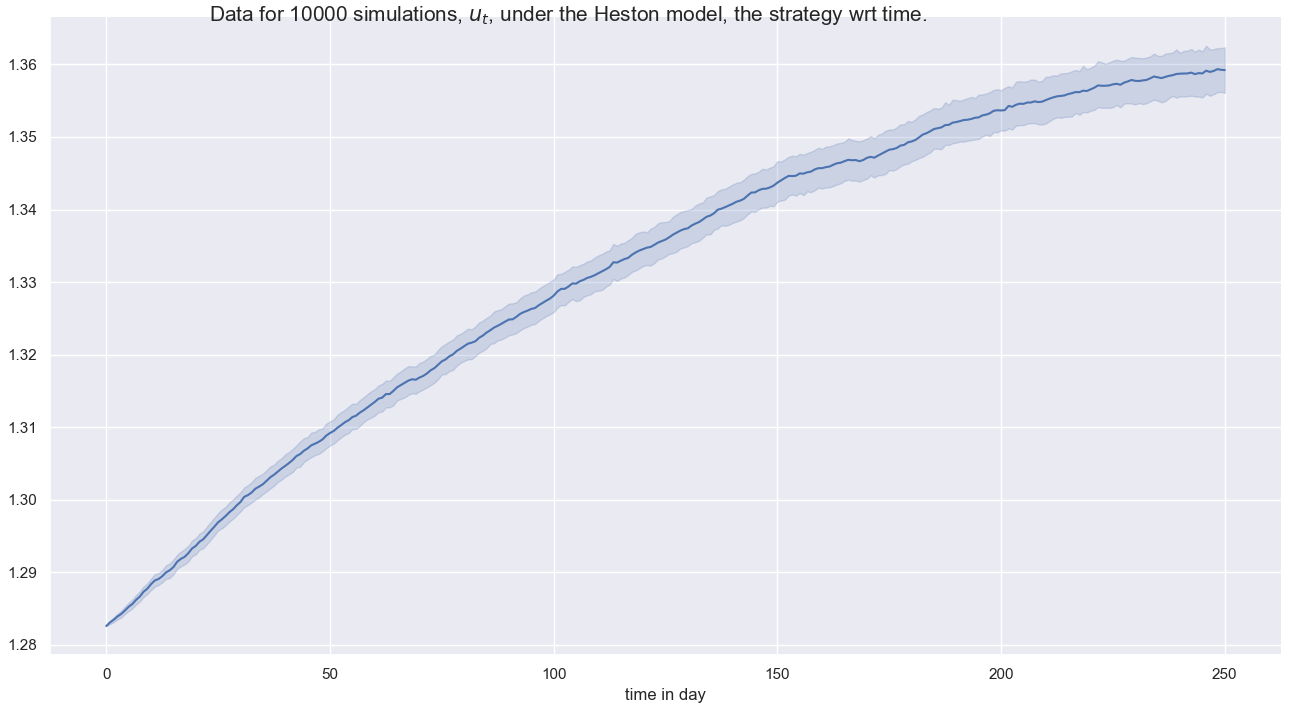
\includegraphics[width = 0.44 \textwidth]{../addition_part/images/numerical_studies/bootstrap_u_t.png}
}}
\subfloat{{
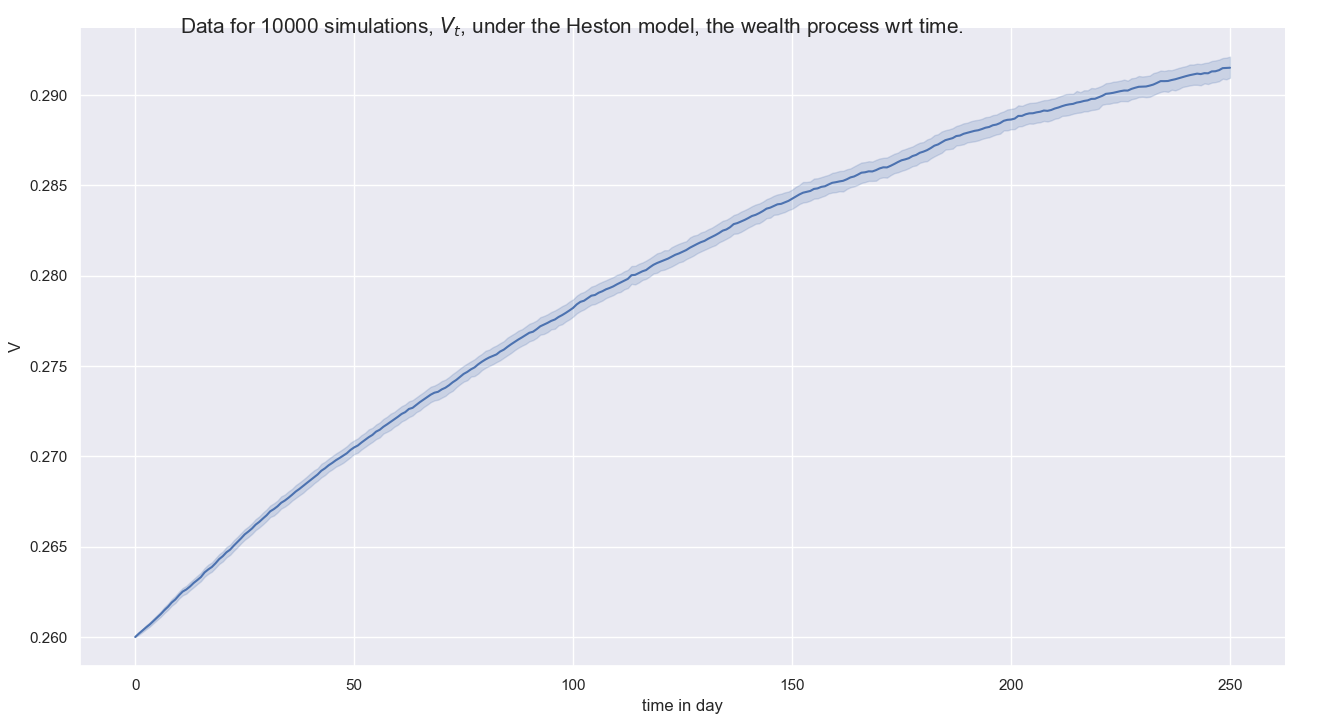
\includegraphics[width = 0.44 \textwidth]{../addition_part/images/numerical_studies/bootstrap_V_t.png}
}}\\
\subfloat{{
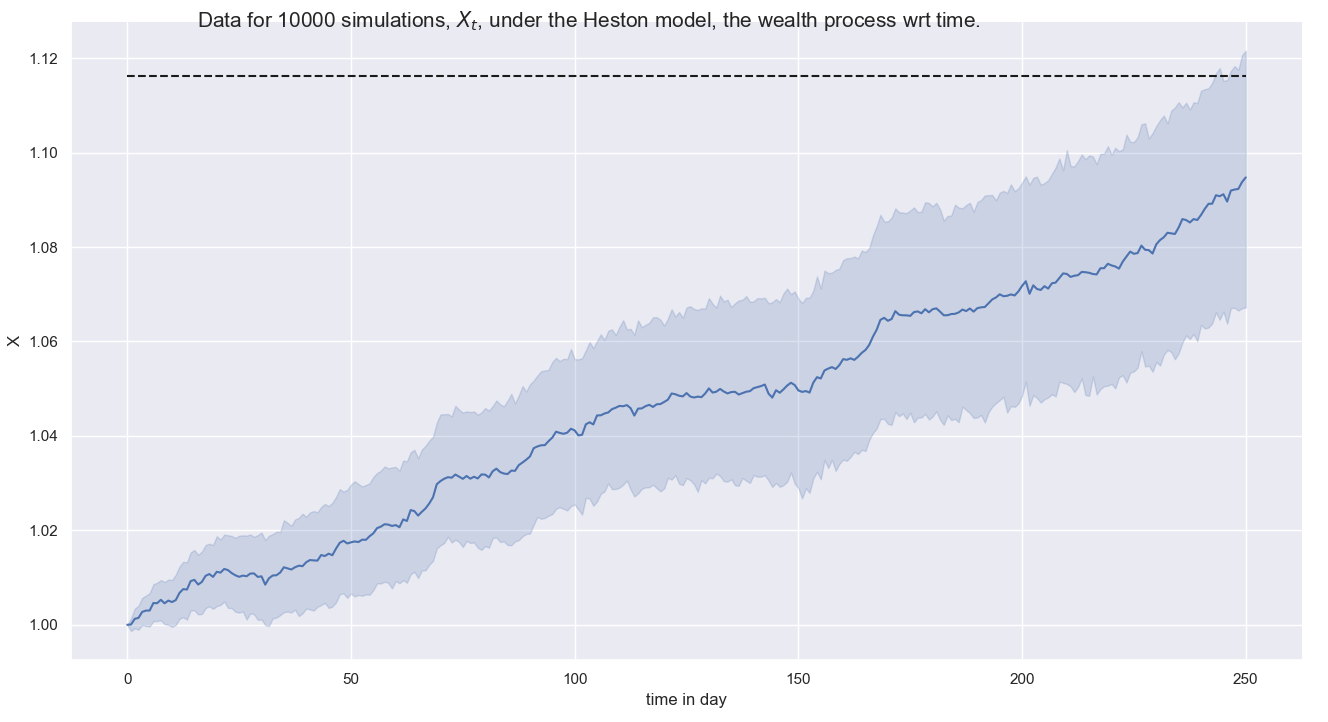
\includegraphics[width = 0.6 \textwidth]{../addition_part/images/numerical_studies/bootstrap_X_t.png}
}} 
\caption{Bootstrap of $10000$ simulations of the normal Heston, displaying the optimal strategy, the volatility, and the wealth.  Set of parameters nb. 1 in \ref{tab:bootstrap}.}
\label{fig:bootstrap}
\end{figure}





\begin{figure}[h]
\centering
\subfloat{{
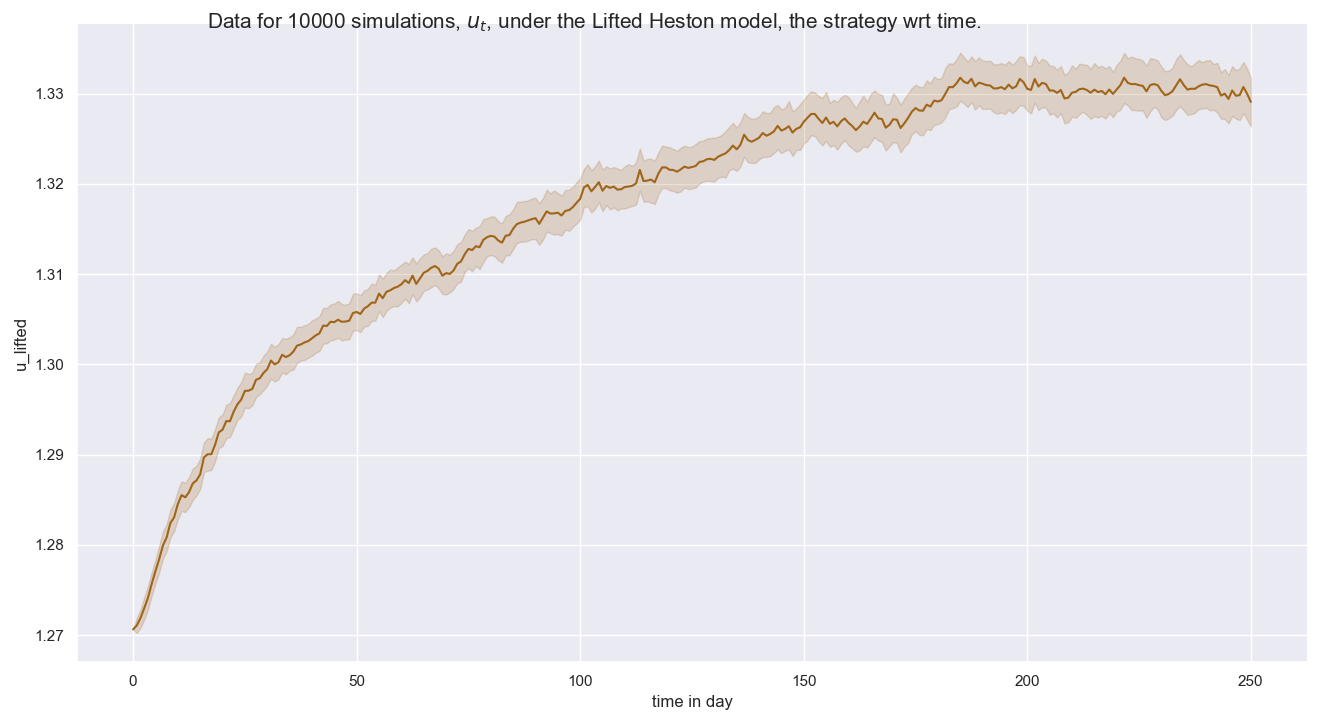
\includegraphics[width = 0.44 \textwidth]{../addition_part/images/numerical_studies/bootstrap_u_t_lifted.png}
}}
\subfloat{{
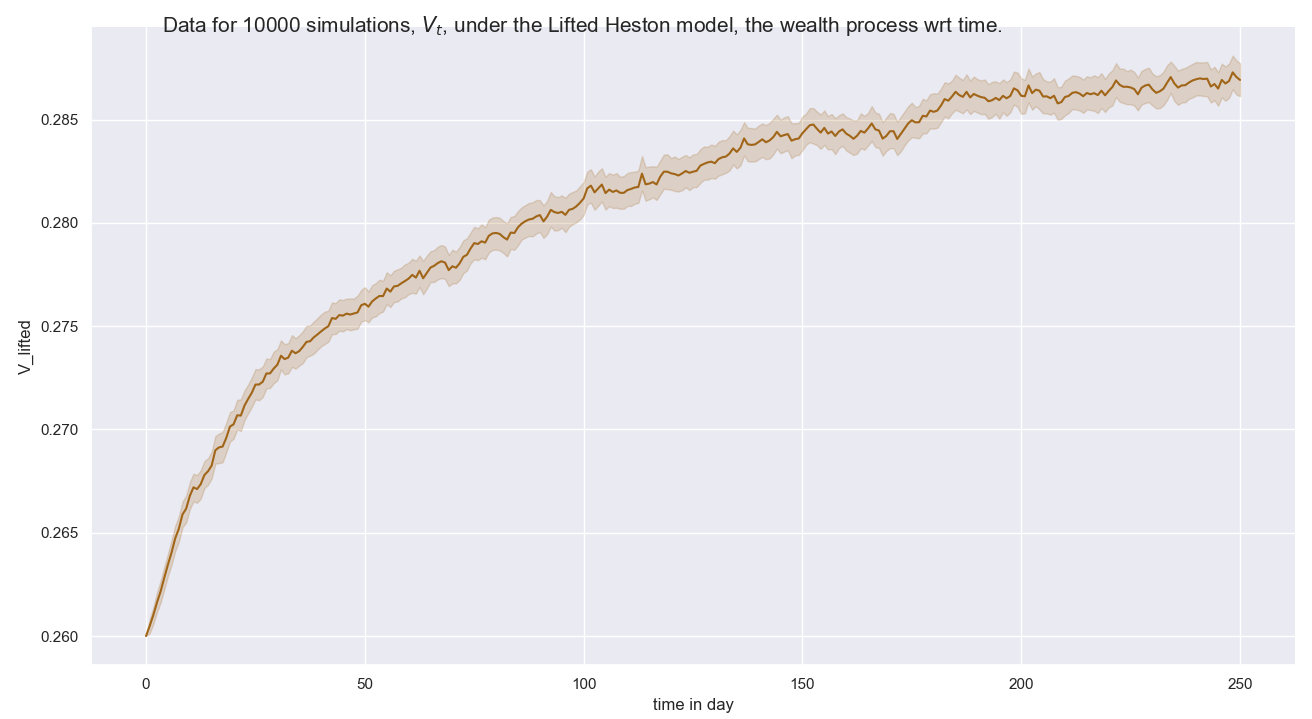
\includegraphics[width = 0.44 \textwidth]{../addition_part/images/numerical_studies/bootstrap_V_t_lifted.png}
}}\\
\subfloat{{
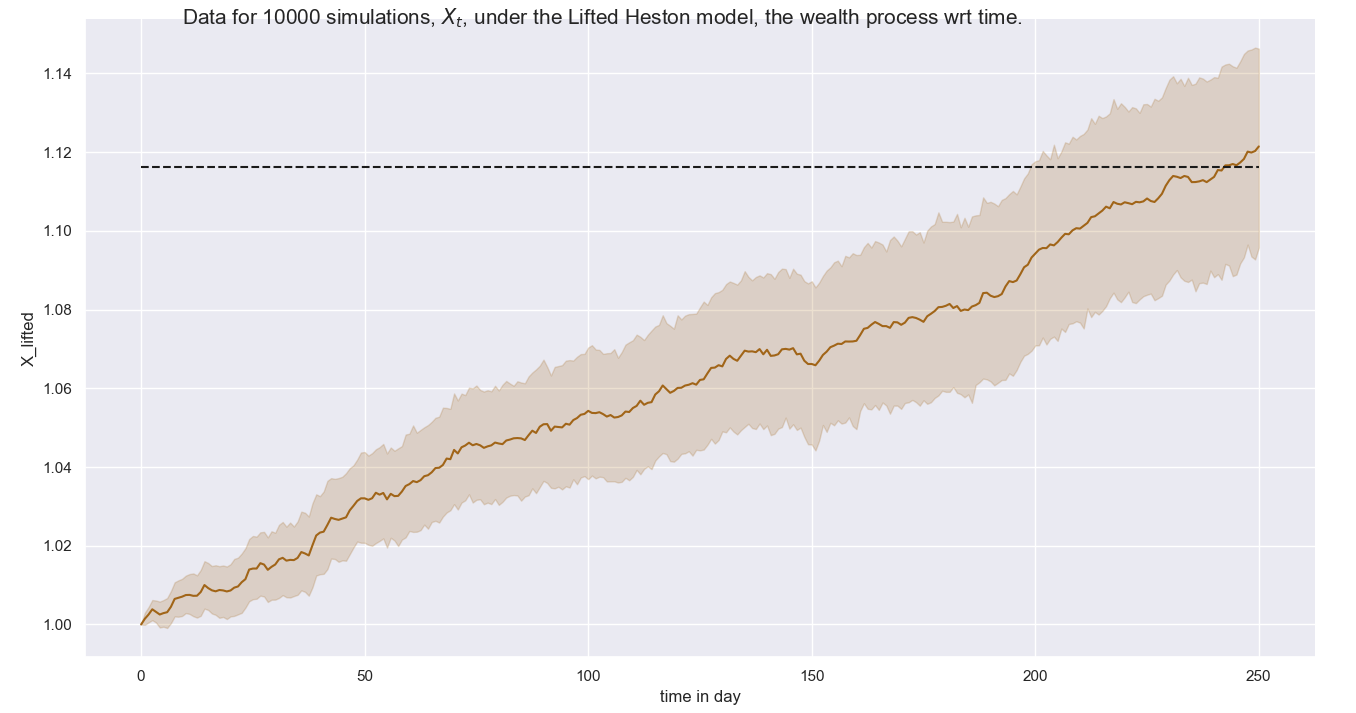
\includegraphics[width = 0.6 \textwidth]{../addition_part/images/numerical_studies/bootstrap_X_t_lifted.png}
}} 
\caption{Bootstrap of $10000$ simulations of the lifted Heston, $\alpha = 0.6 $, displaying the optimal strategy, the volatility, and the wealth. Set of parameters nb. 1 in \ref{tab:bootstrap}.}
\label{fig:bootstraplifted}
\end{figure}





\begin{figure}[h]
\centering
\subfloat{{
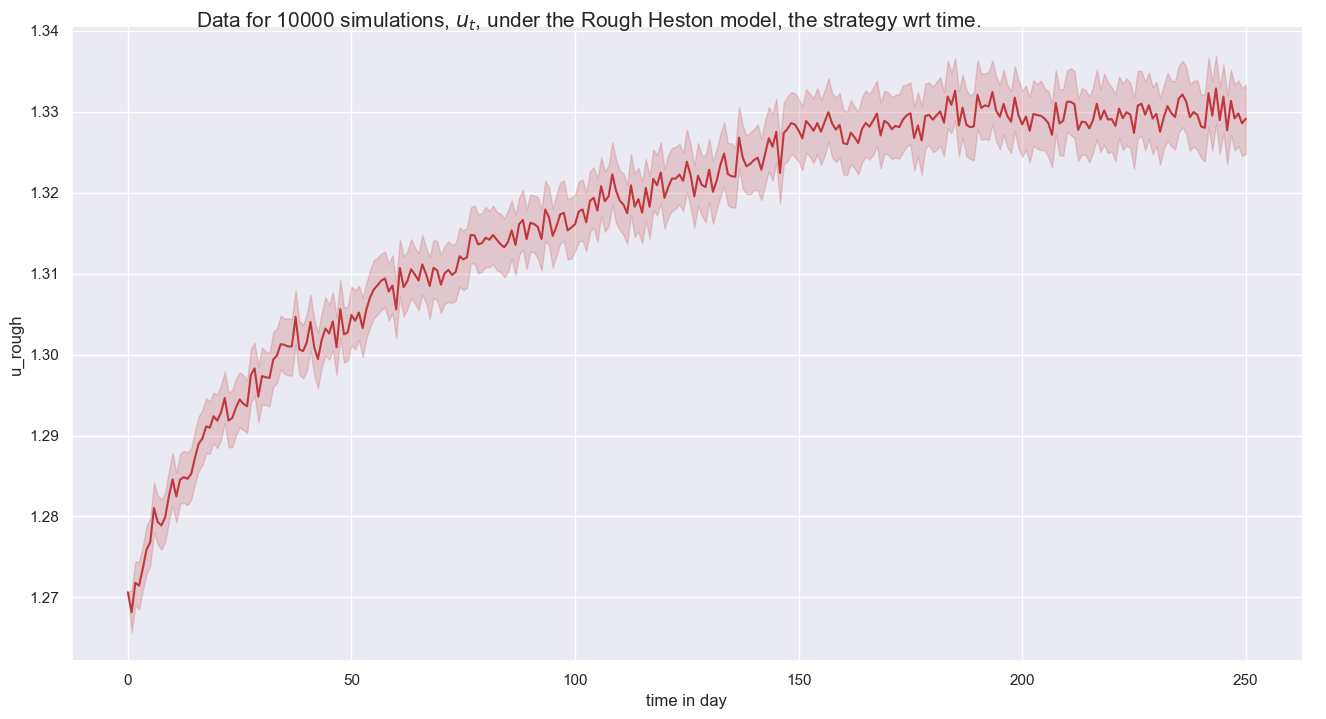
\includegraphics[width = 0.44 \textwidth]{../addition_part/images/numerical_studies/bootstrap_u_t_rough.png}
}}
\subfloat{{
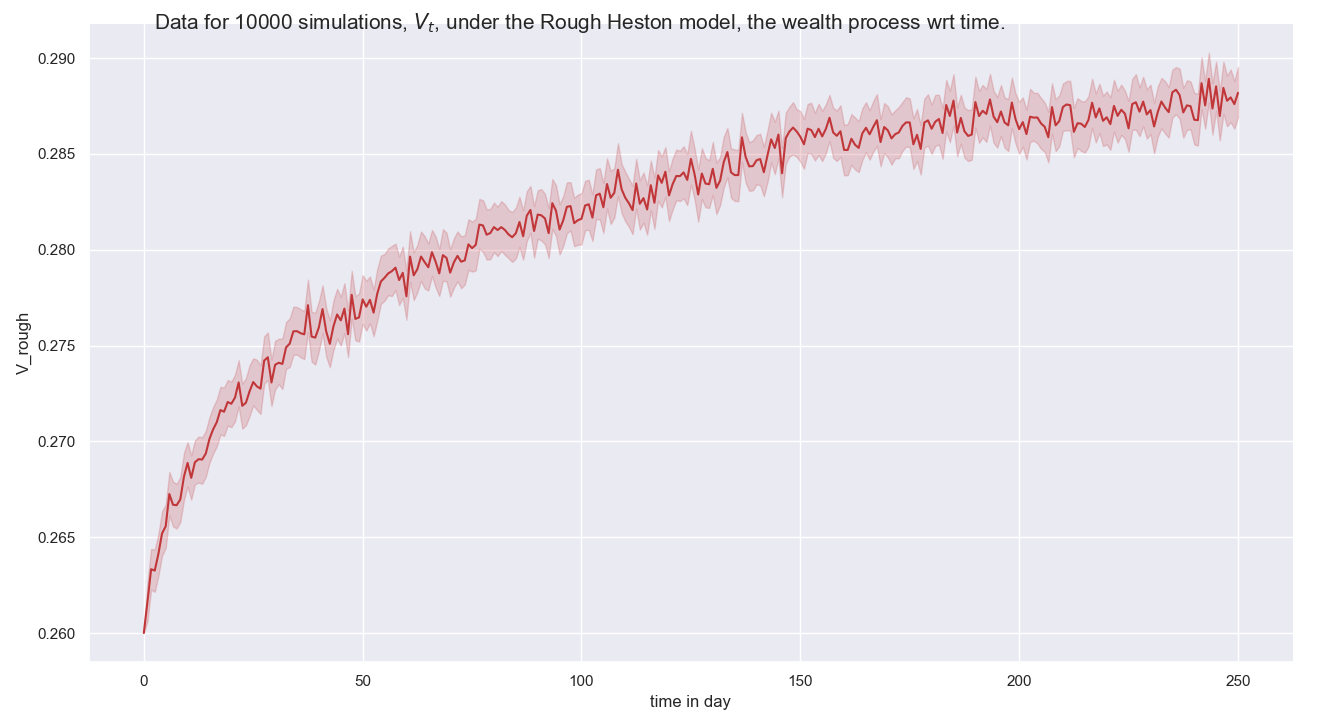
\includegraphics[width = 0.44 \textwidth]{../addition_part/images/numerical_studies/bootstrap_V_t_rough.png}
}}\\
\subfloat{{
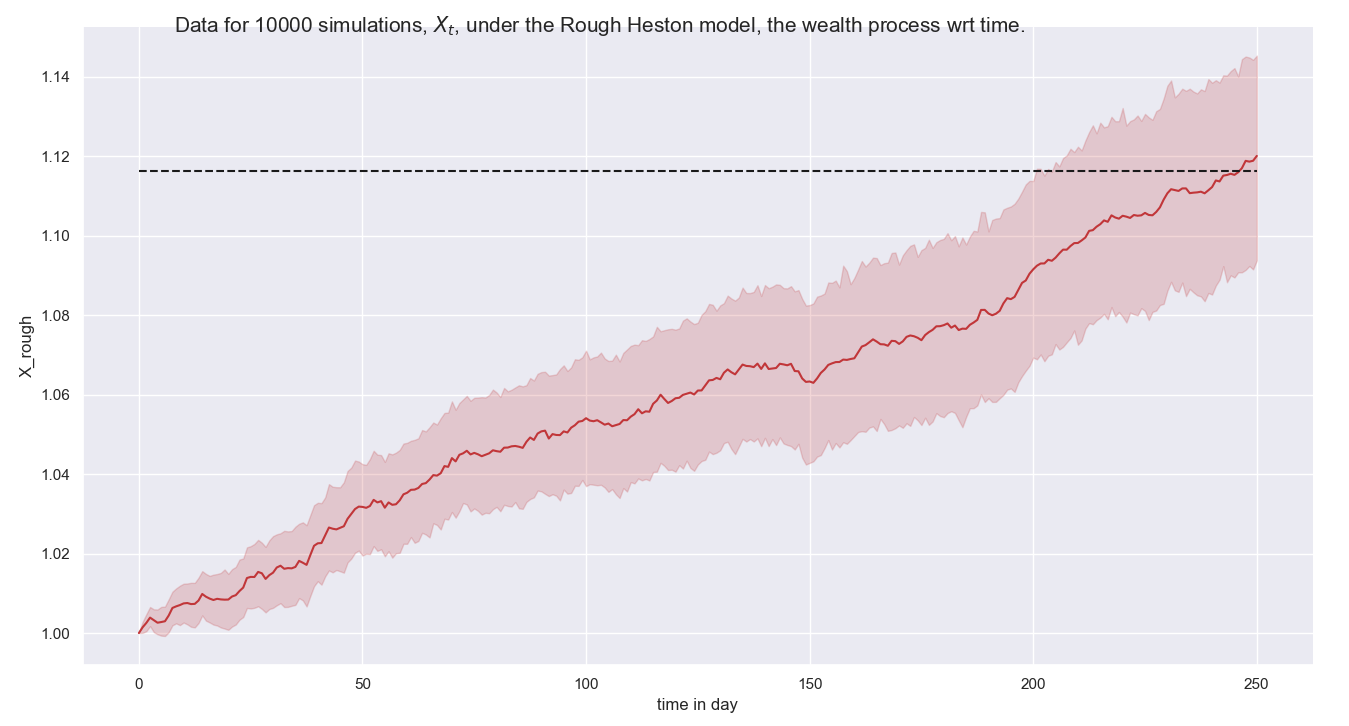
\includegraphics[width = 0.6 \textwidth]{../addition_part/images/numerical_studies/bootstrap_X_t_rough.png}
}} 
\caption{Bootstrap of $10000$ simulations of the rough Heston, $\alpha = 0.6 $, displaying the optimal strategy, the volatility, and the wealth. Set of parameters nb. 1 in \ref{tab:bootstrap}.}
\label{fig:bootstraprough}
\end{figure}




























\begin{figure}[h]
\centering
\subfloat{{
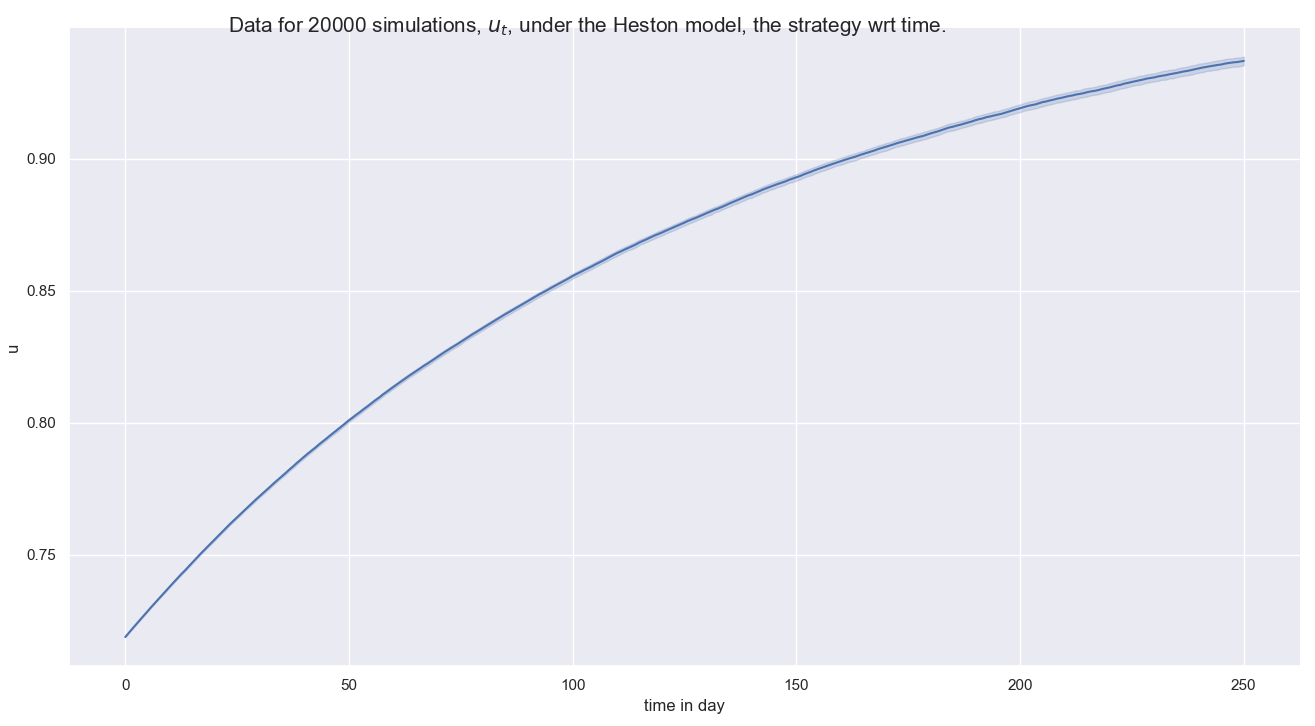
\includegraphics[width = 0.44 \textwidth]{../addition_part/images/numerical_studies/bootstrap_u_t2.png}
}}
\subfloat{{
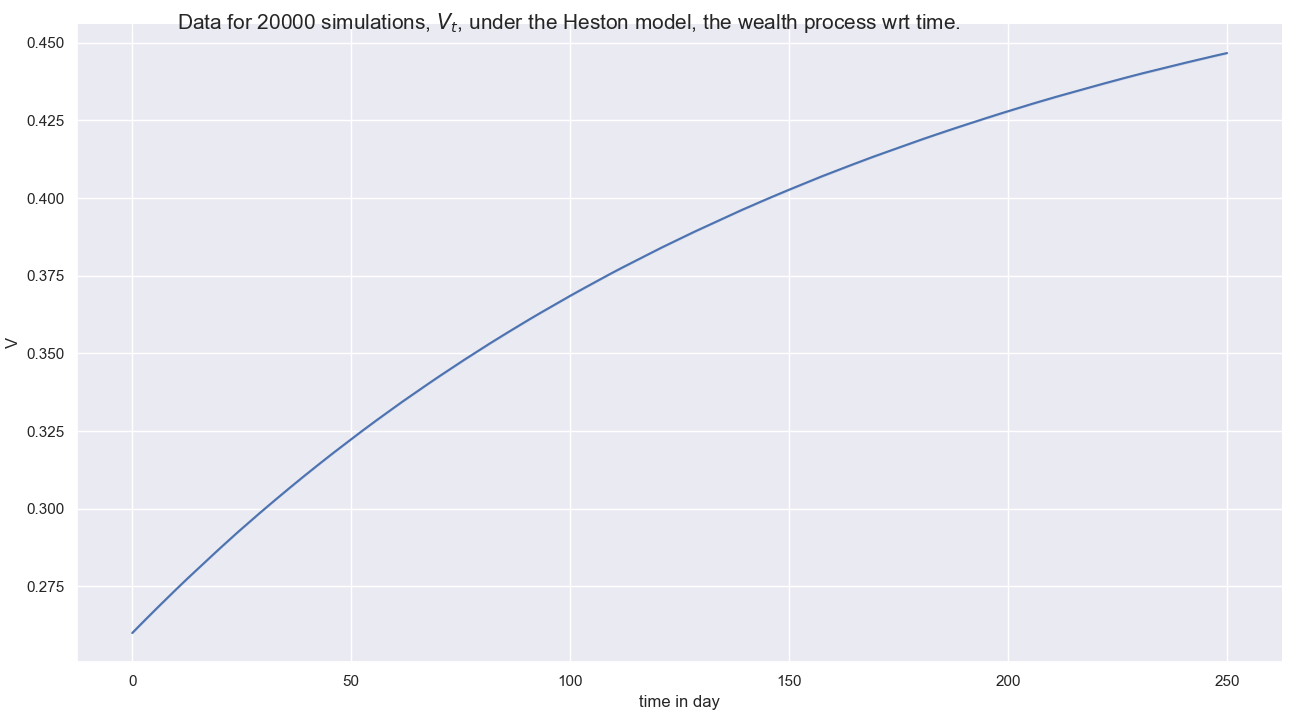
\includegraphics[width = 0.44 \textwidth]{../addition_part/images/numerical_studies/bootstrap_V_t2.png}
}}\\
\subfloat{{
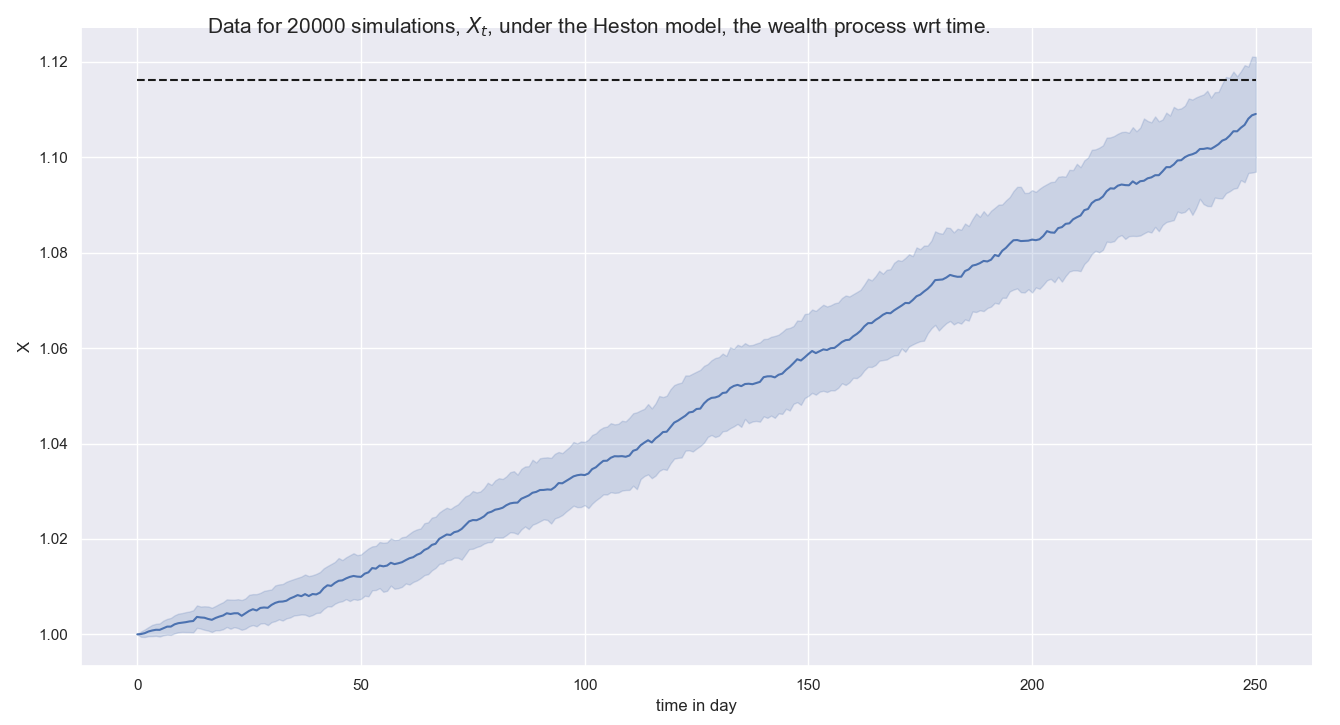
\includegraphics[width = 0.6 \textwidth]{../addition_part/images/numerical_studies/bootstrap_X_t2.png}
}} 
\caption{Bootstrap of $20000$ simulations of the normal Heston, displaying the optimal strategy, the volatility, and the wealth. Set of parameters nb. 2 in \ref{tab:bootstrap}.}
\label{fig:bootstrap2}
\end{figure}





\begin{figure}[h]
\centering
\subfloat{{
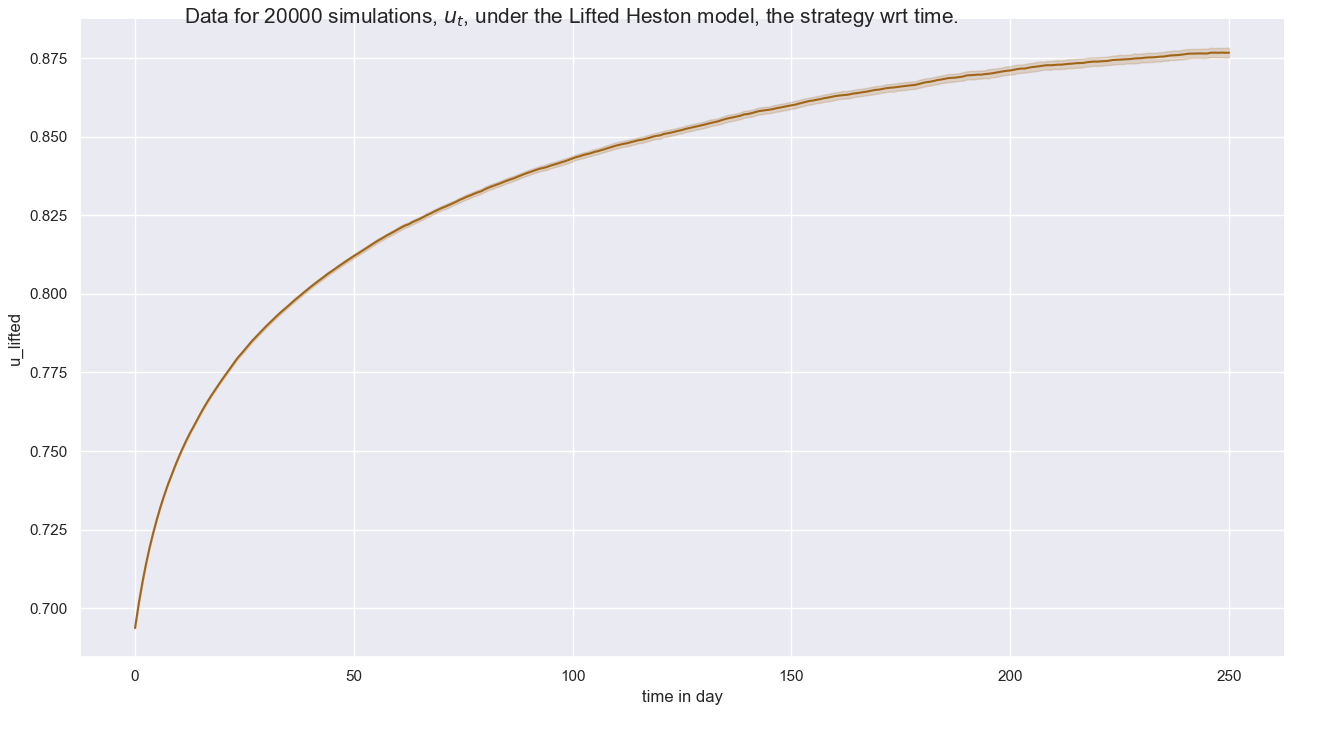
\includegraphics[width = 0.44 \textwidth]{../addition_part/images/numerical_studies/bootstrap_u_t_lifted2.png}
}}
\subfloat{{
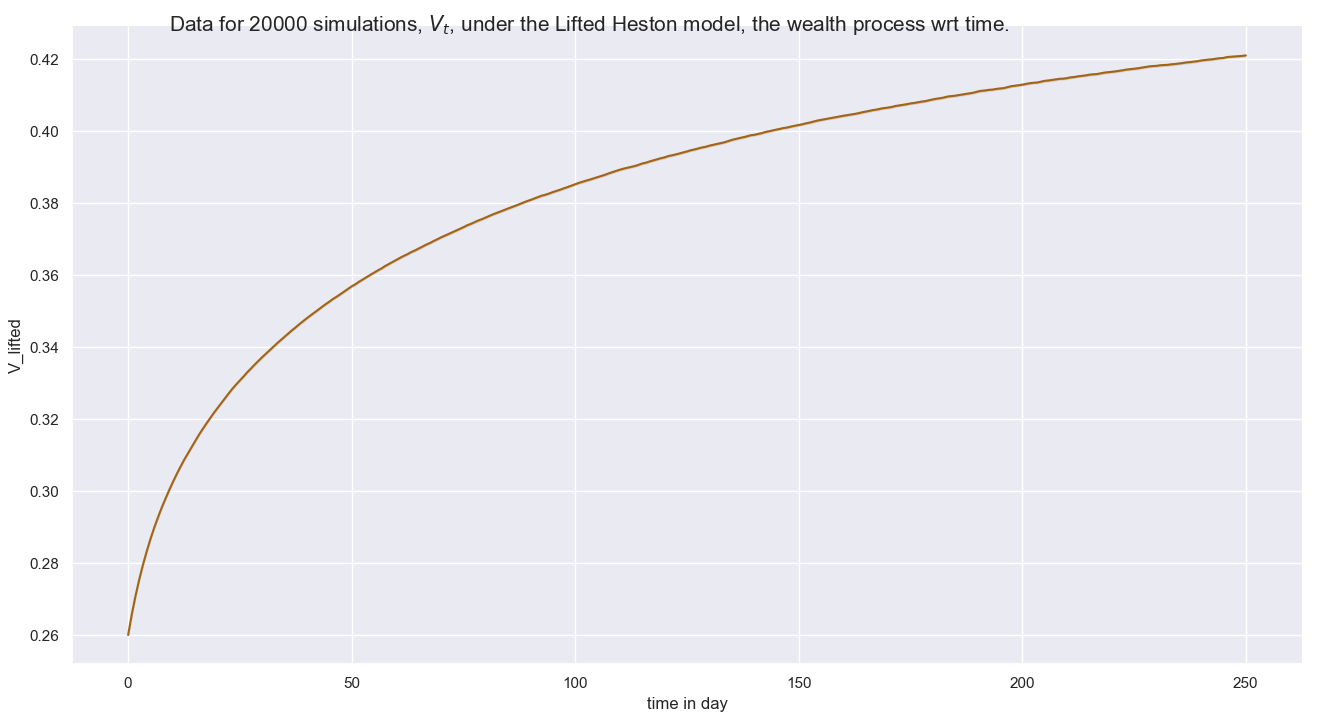
\includegraphics[width = 0.44 \textwidth]{../addition_part/images/numerical_studies/bootstrap_V_t_lifted2.png}
}}\\
\subfloat{{
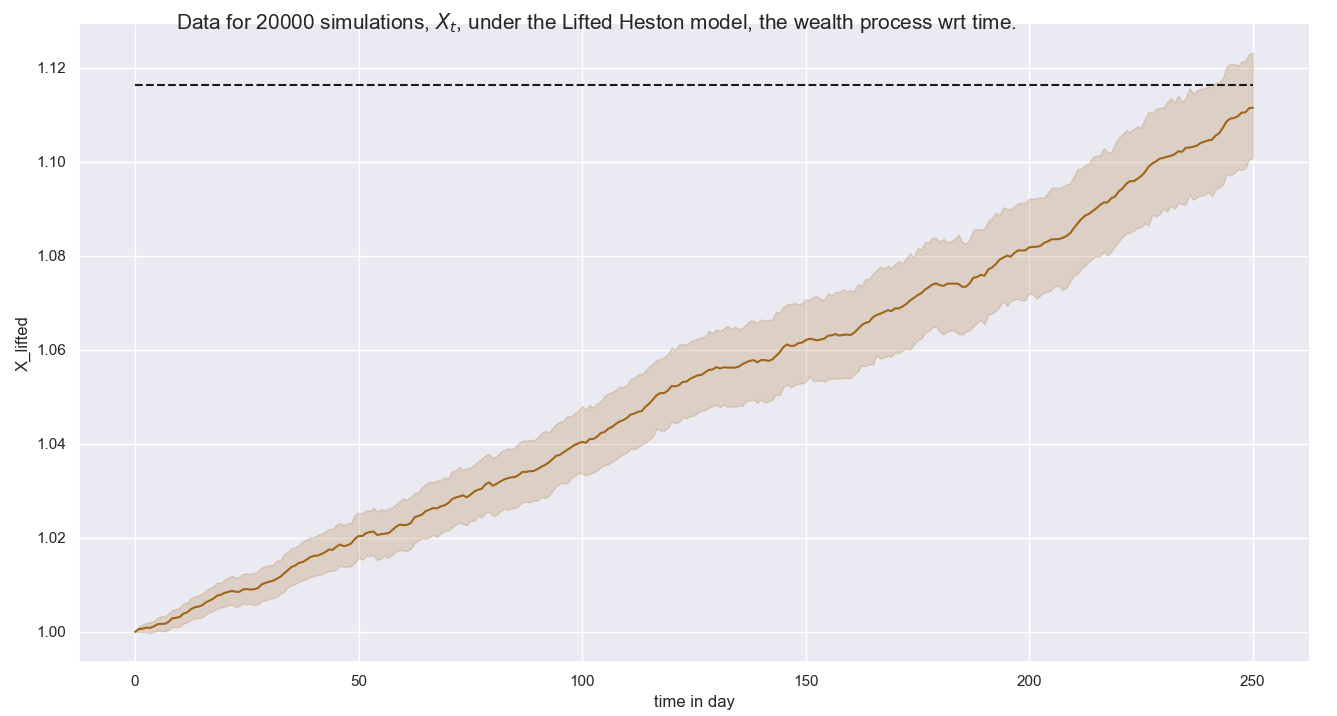
\includegraphics[width = 0.6 \textwidth]{../addition_part/images/numerical_studies/bootstrap_X_t_lifted2.png}
}} 
\caption{Bootstrap of $20000$ simulations of the lifted Heston, $\alpha = 0.6 $, displaying the optimal strategy, the volatility, and the wealth. Set of parameters nb. 2 in \ref{tab:bootstrap}.}
\label{fig:bootstraplifted2}
\end{figure}





\begin{figure}[h]
\centering
\subfloat{{
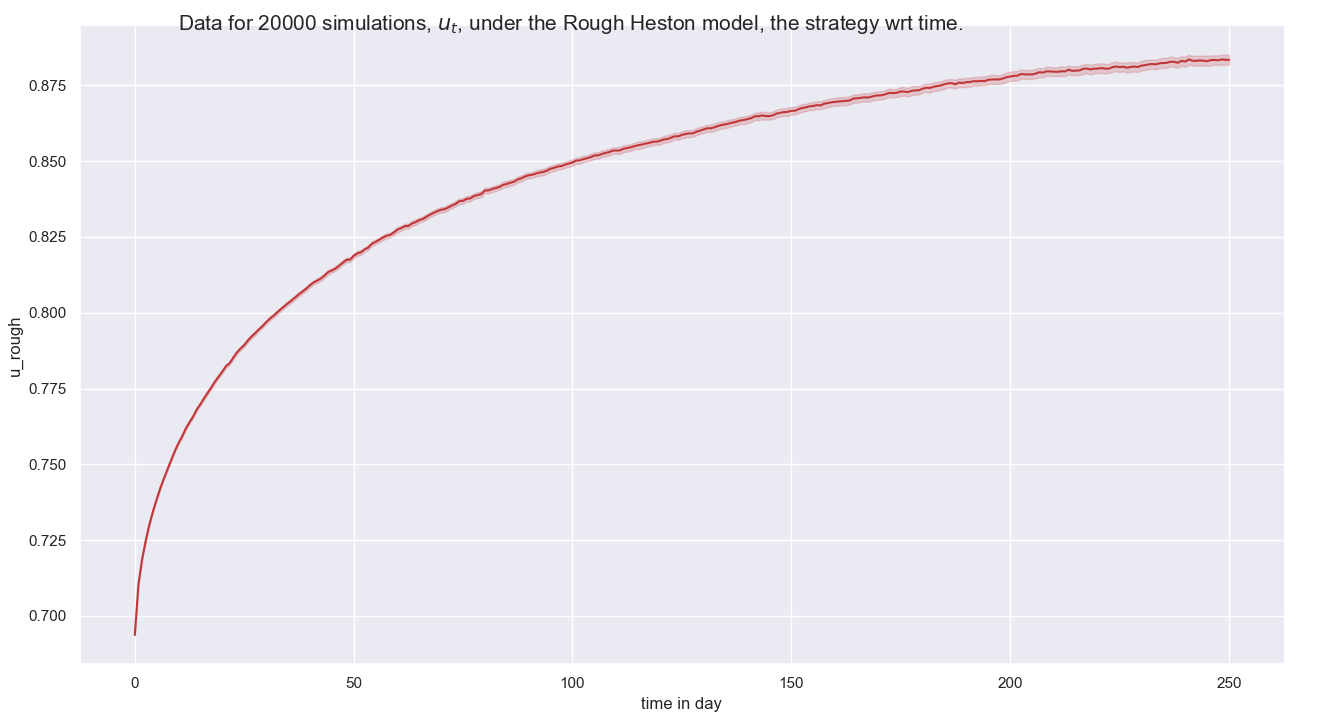
\includegraphics[width = 0.44 \textwidth]{../addition_part/images/numerical_studies/bootstrap_u_t_rough2.png}
}}
\subfloat{{
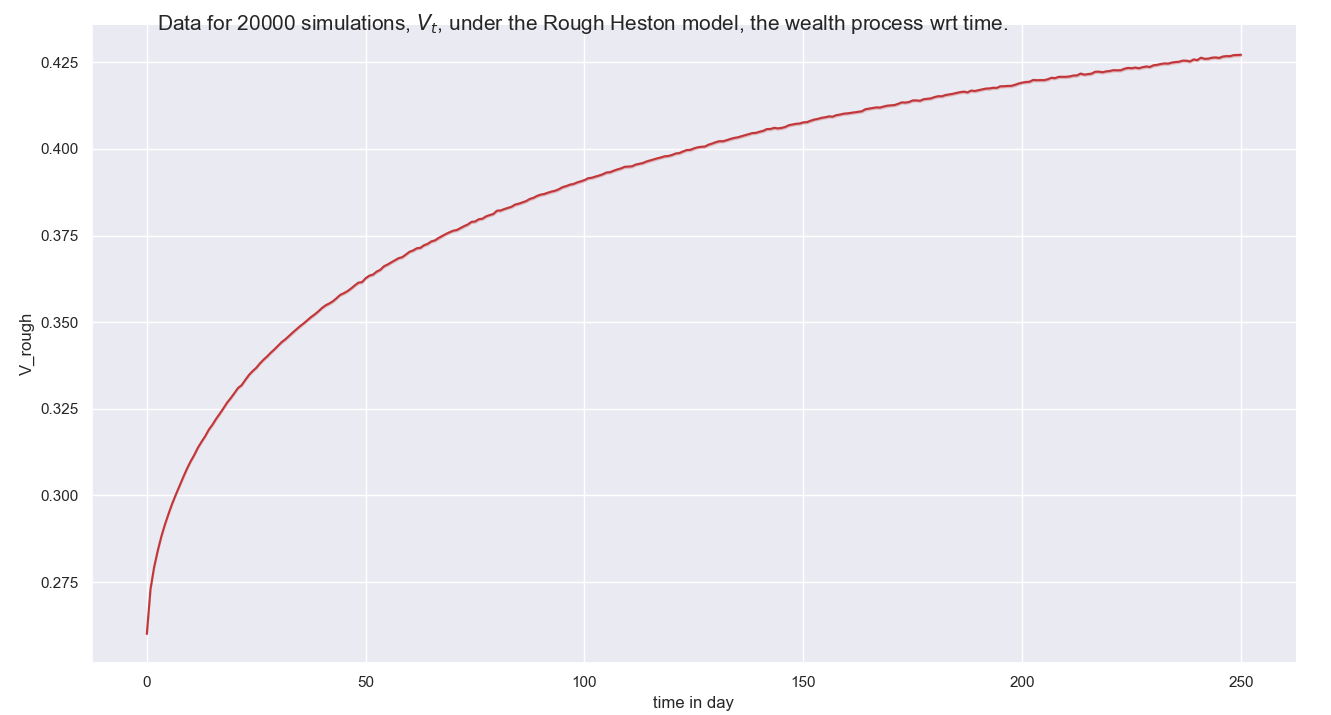
\includegraphics[width = 0.44 \textwidth]{../addition_part/images/numerical_studies/bootstrap_V_t_rough2.png}
}}\\
\subfloat{{
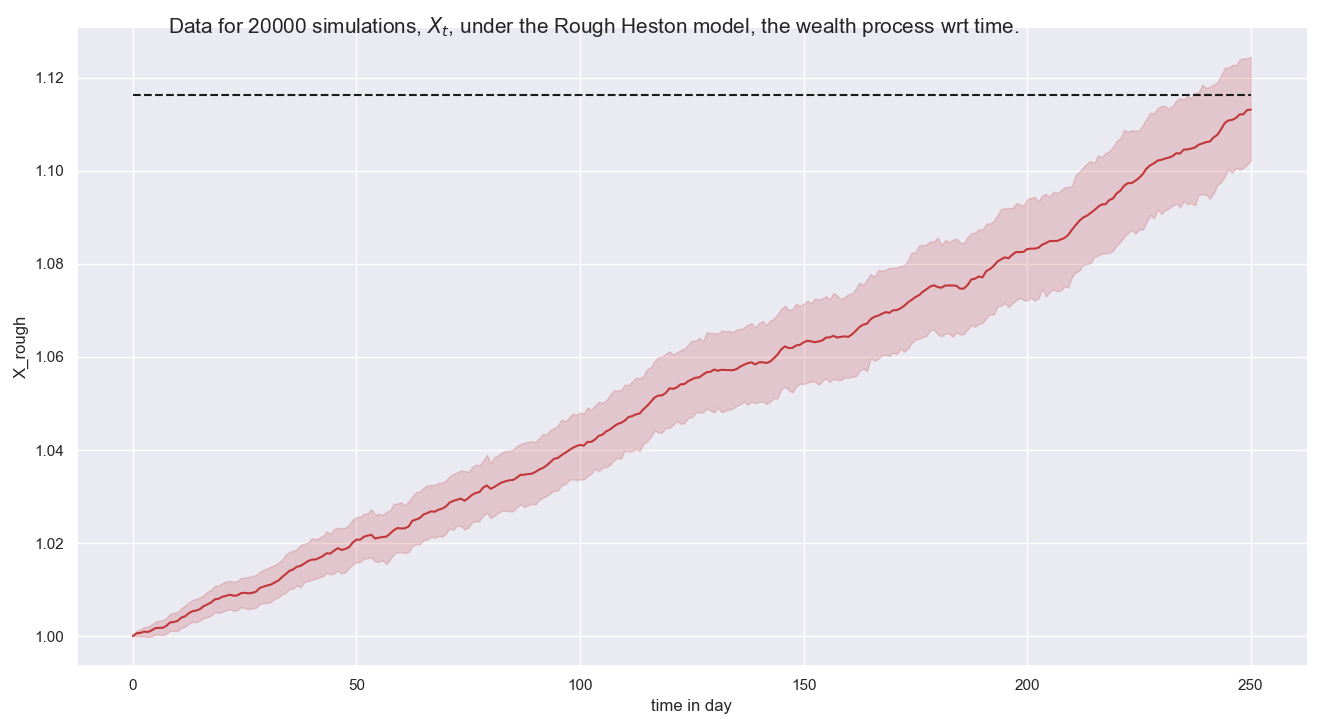
\includegraphics[width = 0.6 \textwidth]{../addition_part/images/numerical_studies/bootstrap_X_t_rough2.png}
}} 
\caption{Bootstrap of $20000$ simulations of the rough Heston, $\alpha = 0.6 $, displaying the optimal strategy, the volatility, and the wealth. Set of parameters nb. 2 in \ref{tab:bootstrap}.}
\label{fig:bootstraprough2}
\end{figure}


\begin{remarque}
In addition to the previous optimistic results, I have also observed that they are heavily dependent on the parameters, and sometimes luck. When $\theta$ is too small, the optimal investment becomes quite instable (due to the fact that the solution to $\psi$ is not that precise anymore) and so the wealth under the classical Heston model fluctuates a lot and does not grow. Also, even though I simulated a big number of paths (20 000), sometimes the results can change from a seed to another, and one gets more payoff from the normal model than from the rough models. 
\end{remarque}

\begin{remarque}
Also, we see on fig. \ref{fig:bootstraplifted} and fig. \ref{fig:bootstraprough} that the expected wealth is higher than the target. It is  for the simple reason that we are simulating the wealth and there is some variance associated to it.
\end{remarque}

\begin{remarque}
Finally, we observe more payoff from Mr. Jacquier's rough model, than from the lifted version, certainly because the former is rougher than the latter.
\end{remarque}


\subsection{Forward Variance }

Forward Variance is a topic I barely scratched. A scheme for simulating it under rough Heston is proposed in \cite{ROUGH_HESTON}.

Here, I will simply recall the definition of it, and give its expression under the Heston model.

\begin{definition}[Forward Variance]
For a process which dynamics is given by the Volterra-Heston equation, with $b_s$ as drift and $\sigma_s$ the volatility, then:
$$ \Theta_u^t := \E \left [ V_u  - 1_{ t \leq u } \cdot  \int_t^u b_s ds  | \mathcal F_t  \right ] $$
\end{definition}

In other words, it is the mean of the expected variance knowing a future state of the world. If one fixes $u < t$, then the forward variance $\Theta_u^t$ reduces to $V_u$.












\chapter{Option Pricing, Heston Model}
\label{chapteroptionpricing}
\section{Introduction}

Now that we are done with Han Wong's paper, we proceed with the understanding of pricing, which is the second numerical topic I approached. We first define what it means to give a price to an asset, and then we price basic options like European call options. 

We go through a few technics, statistical as well as closed form. We also try to optimize those, in order to reduce the complexity of the methods; In particular we use the fft algorithm. All the methods can be generalized for more complex options types, but we will only focus on European call options. Those have the particularity to be easily computed and allows to focus on the technical issues of the methods.

Finally, we discuss quickly how well neural networks are able to approximate Black and Scholes.

\subsection{How to price options ?}

\begin{definition}[European Call Option]
$$C_T(K) :=  \Max (S_T - K, 0) =: (S_T - K)^+   $$
\end{definition}

One way to price financial instruments is to find a price where no arbitrage exists. This range of prices is called the arbitrage free prices. 

Equivalently thanks to the fundamental theorem of asset pricing, the price of any financial instrument, coined here $V_0$, is given by the expectation under a martingale / risk-free measure called $\mathbb Q$ of the discounted financial asset, or in other words for European call options:
$$V_0 = e^{-r T}  \mathbb E_{\mathbb Q} [ (S_T - K)^+ ] $$


\begin{theoreme}{Fundamental Theorem of asset pricing}
A model is said to be arbitrage-free i.e. there does not exist any admissible arbitrage strategy if and only if there exists an equivalent martingale measure $\mathbb Q$.
\end{theoreme}


There can be multiple different prices for the same option, thought in the case of a complete market, the price is unique. Under the Black and Scholes model, the market is complete and for that reason we find a unique price (B$\&$S model: appendix \ref{thrm:BSformula}). 



Also, one can equivalently price call or put option thanks to the put-call parity, which comes from the no arbitrage assumption: 


\begin{theoreme}{Put-Call parity}
$$C_t - P_t = S_t - \frac K {(1+r)^{T-t} }$$
\end{theoreme}











\section{Option Pricing Using Characteristic Functions}
\subsection{Theory}

\begin{definition}[Characteristic function]
The characteristic function is defined as the function associated to the random variable $X$ as:
\begin{align*}
  \phi_X \colon \mathbb R &\to \mathbb C \\
  \xi &\mapsto \mathbb E ( e^{i \xi X} ) 
\end{align*}

One can find some useful properties in \cite{num_methods}. One basic, though important, property that we are going to use is that $\phi_X$ is always hermitian, or formally: 

$$\phi_X( \xi ) = \conj{\phi_X} ( -\xi )$$


\end{definition} 




One classic example is the characteristic function for the dynamic of the asset under the Black-Scholes model:

\begin{equation}
\label{eq:charac_BS}
\phi_{X_t} (\xi) = \exp \left ( i \xi X_0 + ( r - \frac{ \sigma^2}{2}
) i \xi t - \frac{\sigma ^2 \xi ^2 t}{2} \right )
\end{equation}

More details in appendix \ref{anx:charac_BS}.

The advantage of pricing with a formula involving the characteristic function of a process over a formula with its density is that more functions have a useful characteristic function than a PDF. Many models do not allow for a closed-form representation of their density for their stock price process. On the other hand, the characteristic function is available to the class of affine models. Therefore, in many sophisticated models, it is easier to work with characteristics functions instead of using density functions.

Further on, we will need Gil-Pelaez Inversion Theorem (cf. \cite{gil_pelaez}), which states:

\begin{theoreme}{Gil-Pelaez Inversion Theorem}
If F is a one-dimensional distribution function and $\phi \colon \xi \to \int_{\mathbb R} e^{i \xi x} F(dx) $  its characteristic function, then we have the inverse formula for any
continuity point $x$ of $F$:

$$ F(x) = \frac 1 2 - \frac 1 { 2 \pi} \int_{\mathbb R} \frac{e^{- i x \xi } \phi ( \xi )  }  { i \xi }  d \xi $$

\end{theoreme}

Our aim is to write a computable expression for $C_T(k)$.


Remember that, writing $k = \ln(K)$, and $q_T$ is the pdf of $X_T$, the final log price of the asset, one can rewrite the pricing function as:

\begin{align}
C_T( k ) &=  e^{-r T}  \mathbb E_{\mathbb Q} [ (S_T - K)^+ ] \nonumber  \\
&= e^{-rT} \int_k^{\infty} e^x q_T(x) d(x) - K e^{-rT} \int_k^{\infty} q_T(x) dx \nonumber \\
&=: S_0 \Pi_1 - K e^{-r T} \Pi_2 
\label{eq:super_pricing}
\end{align}

(\ref{eq:super_pricing}) is, in the literature, usually referred as the "generalized" Black Scholes formula.

Also, remember that by hermitianity of $\phi_T$, one notices that:

$$ \mathfrak{R} ( \phi_T ( \xi) ) = \frac 1 2 \left ( \phi_T (\xi) + \phi_T (-\xi) \right ) \qquad  \text{ and } \qquad \mathfrak{I} ( \phi_T ( \xi) ) = \frac 1 {2i} \left ( \phi_T (\xi) - \phi_T (-\xi) \right ) $$

Gil-Pelaez inversion theorem applied to our pricing equation gives:

\begin{equation}
\label{eq:Pis}
\Pi_1 =  \frac 1 2 + \frac 1 {\pi} \int_0^{\infty} \mathfrak{R} \left ( \frac{ \phi_T ( \xi - i )  }  { i \xi \phi_T(-i) } e^{- i k \xi } \right ) d \xi  \qquad
\text{  and  }  \qquad
\Pi_2 =  \frac 1 2 + \frac {1} {\pi} \int_0^{\infty} \mathfrak{R} \left (  \frac{ \phi_T ( \xi )}    { i \xi } e^{- i k \xi } \right ) d \xi
\end{equation}

Using the function "real part" $ \mathfrak{R} $ allows to reduce truncation errors while computing an improper integral. 

Also, we used that $\phi_T(-i) = 1$. Remember

$$ \mathbb E ( e^{X_T} ) = \E ( S_T ) = S_0 $$ since we are working under the risk neutral measure for $S_t$.


Now, one is able to compute the price $C_T(k)$ by using (\ref{eq:Pis}) inside (\ref{eq:super_pricing}). This method presents two main advantages:

\begin{itemize}
\item \textbf{Generality:} For any process whose characteristic function is known, that method works.
\item \textbf{Semi-analytical solution:} by using integration routines, it is fairly easy to compute the pricing. Semi-analytical means the expression is in the form of the integral / Laplace or Fourier Transform of an analytical function. Numerical integration is described in the next section. 

\end{itemize}














\subsection{Integration}
\label{integration}

In order to compute $\Pi_1$ and $\Pi_2$, we need to integrate numerically a function. 

We are going to describe two different integration routines. For more details one can refer to the lecture notes of my second year lecture: in \cite{annalisa}, as well as in \cite{num_methods}. 

\begin{theoreme}{Trapezoidal Method}
$$\int_a^b f(x) dx = \frac 1 2 (f(a) + f(b))$$
It is first order exact and has the advantage of being extremely easy to use. For well-behaved functions (meaning whose second order derivates do not explode), the error is $ o (\frac 1 {n^2})$
\end{theoreme}


\begin{theoreme}{Simpson's Rule}
$$\int_a^b f(x) dx = \frac 1 6 (f(a) + 4 f(\frac{b-a}{2}) + f(b))$$
Simpson's method is much more precise as this method is third order exact and its error is $o (\frac 1 {n^4})$.
\end{theoreme}

\begin{remarque}
While trapeze's error is related to the second derivative of the function, Simpson's error is related to the fourth order derivative; more details in \cite{annalisa}. 
\end{remarque}


\begin{figure}
\centering
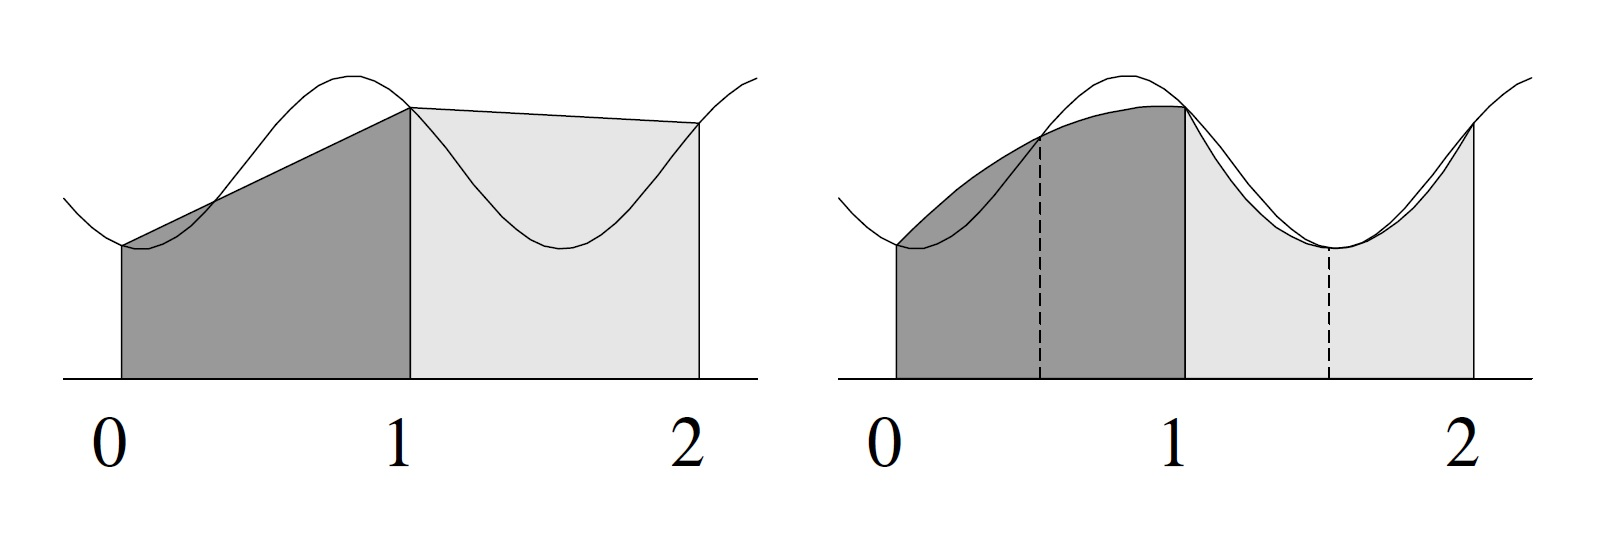
\includegraphics[width = 0.5 \textwidth]{../addition_part/images/integration_fft/numerical_integration.jpg}
\caption{Graphical explanation of the two quadratures method, images from \cite{annalisa}. Left: trapezoidal quadrature, right: Simpson's method.}
\end{figure}









\subsection{Overview of the different methods}
In order to compute the integrals, one needs the evaluation of the integrand at the desired points. Under the Heston model, we are lucky to have a closed form formula. However, as a first step, let me present a (failing) method to estimate the characteristic method. Another better and faster option for estimating the price is to directly compute the empirical price. The latter method is presented in section \ref{empirical_price}.

\subsection{Estimation of the characteristic function }


Following the definition of the characteristic function, one can estimate $\phi_X$ by estimating the PDF of the asset at maturity. Indeed, remember that:

$$\phi_{X_T} (\xi) = \mathbb E [ e^{i \xi X_T } ] = \int_{\mathbb R} e^{i \xi x } f_{X_T}(x) dx $$

I thought about two estimation methods:

\begin{itemize}
\item discrete: one approaches the PDF by the histogram. A classical result from statistics proves that the histogram of a random variable converges in probability to its PDF under certain conditions (cf. \cite{panaretos}).
\item continuous: using KDE, one can smoothen up the histogram and get a continuous PDF that should be close to the true PDF for the same reasons.
\end{itemize}

Figure \ref{fig:histogram_S} shows all the simulated final realisations of the process. 





\begin{figure}
\centering
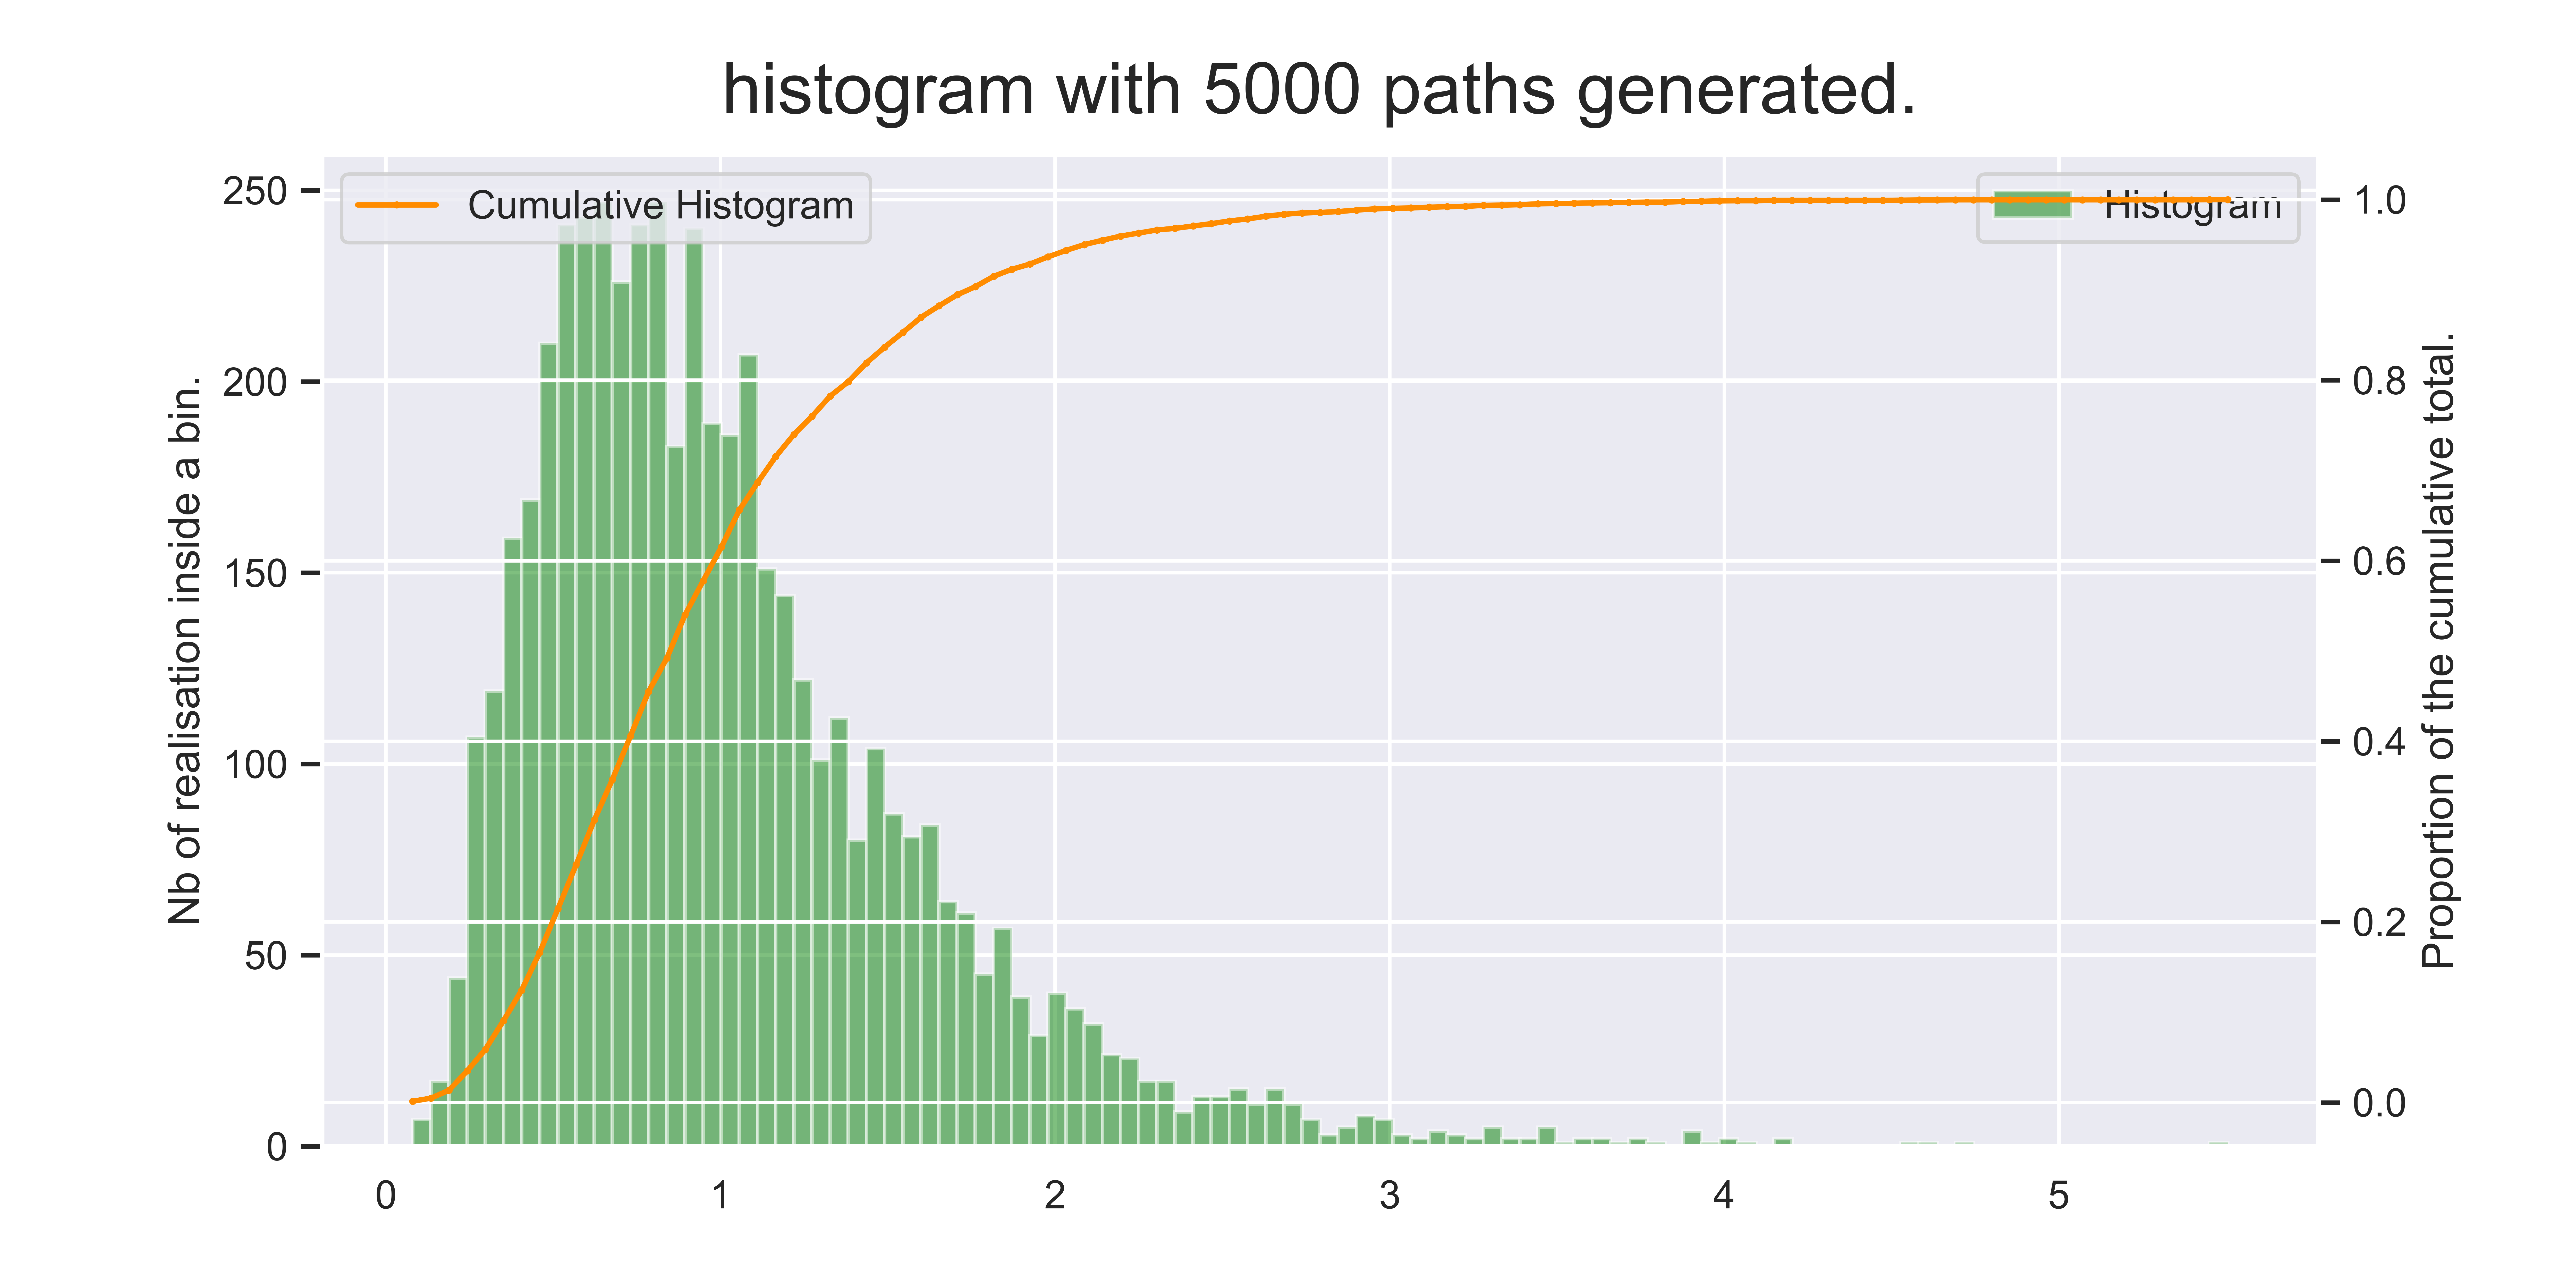
\includegraphics[width = 0.8 \textwidth]{../addition_part/images/integration_fft/histogram_real.png}
\caption{Histogram of the final realisations of the simulated process.}
\label{fig:histogram_S}
\end{figure}

Based on that histogram, KDE algorithm has been applied leading to the figure \ref{fig:histogram_S_KDE}.




\begin{figure}
\centering
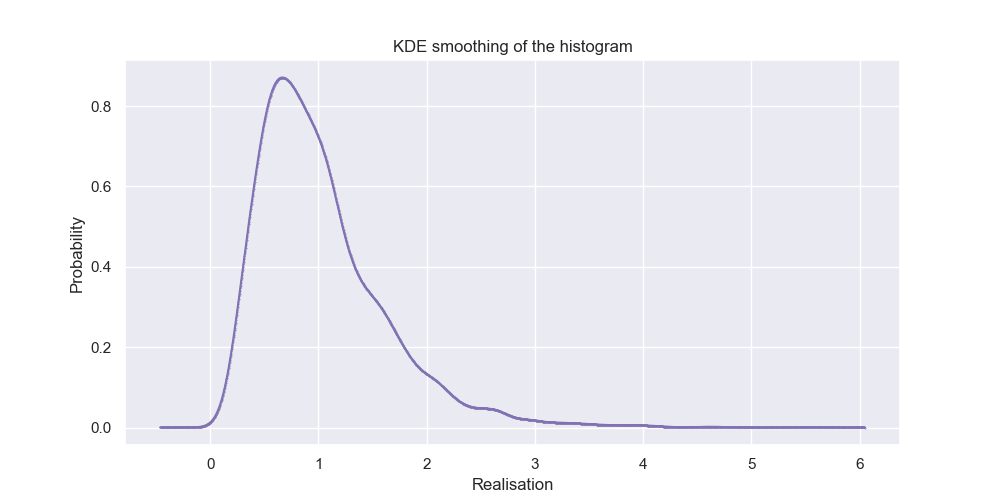
\includegraphics[width = 0.7 \textwidth]{../addition_part/images/integration_fft/histogram_real_kde.png}
\caption{KDE applied upon the histogram fig. \ref{fig:histogram_S}.}
\label{fig:histogram_S_KDE}
\end{figure}











\subsection{Results for continuous estimation} 

\begin{table}
\begin{center}
\begin{tabular}{   m{4.5 cm} | m{4.5 cm}   } 
\hline
Parameter & Value \\ 
\hline
\hline
$\sigma$ & 0.1  \\
\hline
$V_0$ &  0.1 \\
\hline
$X_0$ &  1 \\
\hline
$r$ & 0.0 \\
\hline
$\rho$ & -0.56 \\
\hline
$\theta$  & 0.07  \\
\hline
$\kappa$ & 1 \\
\hline
$\phi$ & 1  \\
\hline
T & 3 \\
\hline
\end{tabular}
\caption{Set of parameters for the estimation of the characteristic function.}
\label{table:kde}
\end{center}
\end{table}

In this section, as well as for the discrete estimation, we use the parameters described in table \ref{table:kde}.


First the following figures show the integrands at a chosen strike price: figure \ref{fig:integrand_kde}. Plotting the integrands is a crucial step in order to choose the domain of integration. The domain of integration has to be chosen manually in order to reduce integration errors. My strategy was to observe the integrands for a few strike prices, and pick the max where the function is non zero. Then to this value I add some leeway, in case I wasn't exactly accurate.

\begin{figure}
\centering
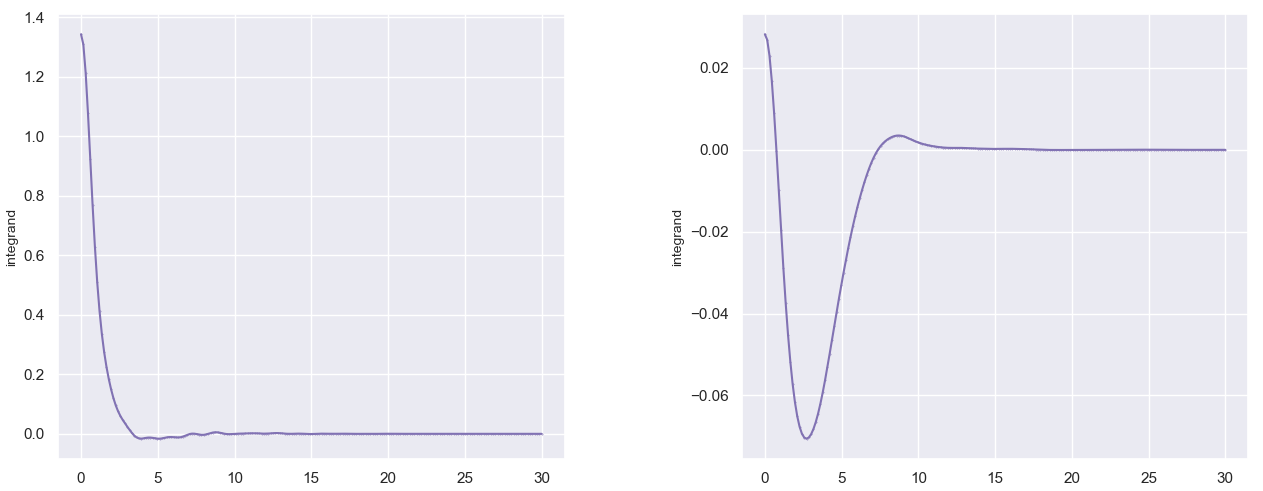
\includegraphics[width = 0.8 \textwidth]{../addition_part/images/integration_fft/kde_integrand.png}
\caption{Integrands for (\ref{eq:Pis}) by KDE, where the observed log strike price is equal to one. $\Pi_1$ on the left, $\Pi_2$ on the right.}
\label{fig:integrand_kde}
\end{figure}

The plot of the pricing with respect to the log-moneyness can be seen figure \ref{fig:price_kde}.


\begin{figure}
\centering
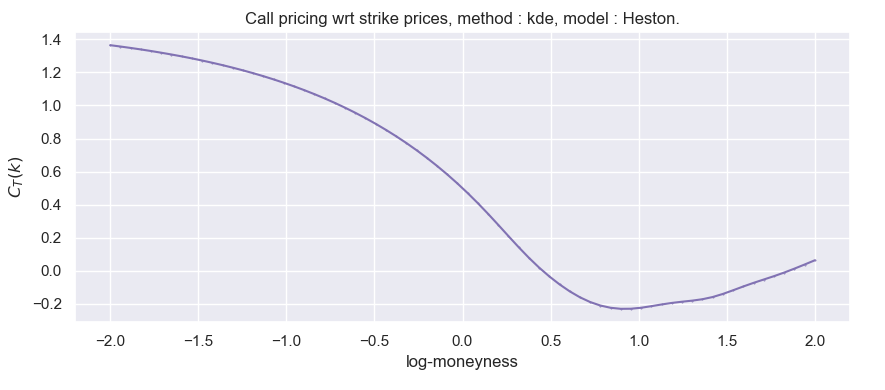
\includegraphics[width = 0.7 \textwidth]{../addition_part/images/integration_fft/pricing_kde.png}
\caption{Pricing using the KDE approximation parameters in table \ref{table:kde}.}
\label{fig:price_kde}
\end{figure}

About the code, one has to be careful using the KDE with the choice of the bandwidth. Here, the automatic choice from scipy wasn't really helpful. By a method of trial and error, I found the most suitable one.

\textbf{Observations : }

We analyze the integrands by comparing them to the closed form in subsection \ref{comparaison_integrands}.

About the price, first we observe that there are some negatives prices, therefore it is blatantly wrong. A comparison with respect to the true prices is written in subsection \ref{comparaison_price}.












\subsection{Discrete estimation of the characteristic function}

As introduced in the previous subsection, one can compute the characteristic function by a discrete method. In the exact same way, the integrands are shown on fig. \ref{fig:integrand_moments}.

\begin{figure}
\centering
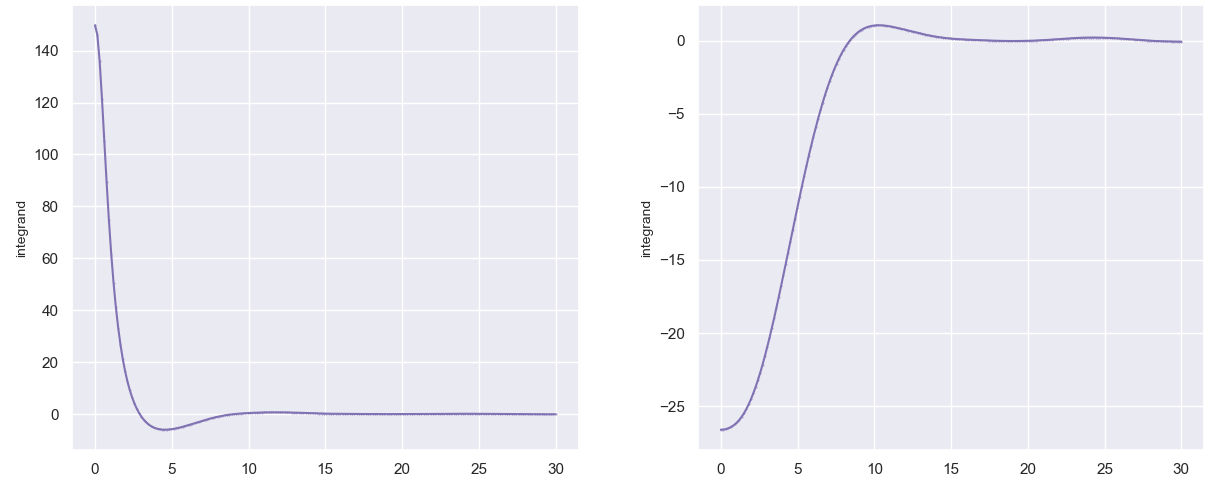
\includegraphics[width = 0.8 \textwidth]{../addition_part/images/integration_fft/moments_integrands.png}
\caption{Integrands for (\ref{eq:Pis}) by moment approximation, where the observed log strike price is equal to one. $\Pi_1$ on the left, $\Pi_2$ on the right.}
\label{fig:integrand_moments}
\end{figure}


I also wanted to plot the pricing, however the program doesn't end. The first strike prices took an extremely long time to compute, and then the computations stopped in the middle of the strike prices. As one can see on the integrands, they explode near $0$ and my guess is that for certain strike prices the function is not numerically integrable. For whatever reason the bug appears, it is not interesting to delve in that direction as we saw that the integrands are totally wrong. 














\subsection{Empirical Pricing}
\label{empirical_price}
The previously shown statistical methods weren't conclusive. Before dealing with the closed form, here is an attempt to \textbf{correctly} estimate the price. Since we couldn't find the closed form formula for an expression involving a risk premium, we set $\theta = 0$ in this section, for comparison sake.

Our target is to estimate the price of a European call option:
$$V_0 = e^{-r T}  \mathbb E_{\mathbb Q} [ (S_T - K)^+ ] $$

By weak law of large numbers, that we remind here:

\begin{theoreme}{Weak Law of Large Numbers \cite{panaretos}}
When $X_n$ is i.i.d. such that $\mathbb E [ X_n ] = \mu < \infty $, and defining  $ \overline{ X_n } := \sum^n_1 X_i $, then:

$$ \overline{X_n} \xrightarrow[]{p.} \mu $$ 
\end{theoreme}

as well as by Slutsky theorem:

\begin{theoreme}{Slutsky Theorem \cite{panaretos} }
$X_n$ and $Y_n$ random variables, $c \in \mathbb R$.
Let's define a function $g \colon \mathbb R^2 \to \mathbb R$, continuous for the first variable on $\mathcal X$ such that $P(X \in \mathcal X) = 1$. We also need that :

\begin{align*}
\overline{X_n} &\xrightarrow[]{d.} X,  \\
\overline{Y_n} &\xrightarrow[]{p.} c.
\end{align*}

Then, Slutsky has shown that: 

$$ g(X_n, Y_n)\xrightarrow[]{d.} g(X,c)$$

\end{theoreme}


then, by defining a new stochastic process as the payoff of a call option at strike price $K$ and maturity $T$, we get that $\overline{X_n}$ converges in distribution to the true expectation. 

Those theoretical results ensure convergence for a big number of simulations (How big? empirical answer on fig. \ref{fig:IVempirical_evol}). Thus, one can compute the "empirical pricing", and has the results visible on fig. \ref{fig:simulations_empirical_pricing} and fig. \ref{fig:simulations_empirical_pricing}. The parameters are the ones from the next section, namely set 1: table \ref{table:parameters_for_closed_form}. 

\begin{figure}
\centering
   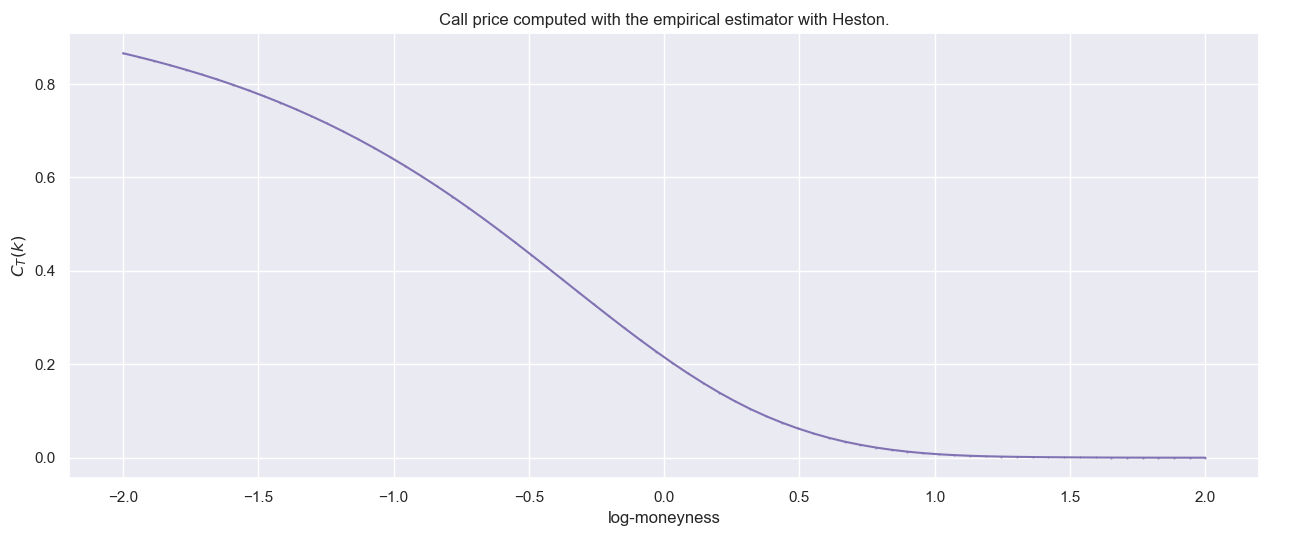
\includegraphics[width = 0.8 \textwidth]{../addition_part/images/integration_fft/empirical_pricing_5000.png}
   \caption{Pricing with the empirical estimator, 20000 simulations.}
   \label{fig:simulations_empirical_pricing}
\end{figure}


\begin{figure}
\centering
   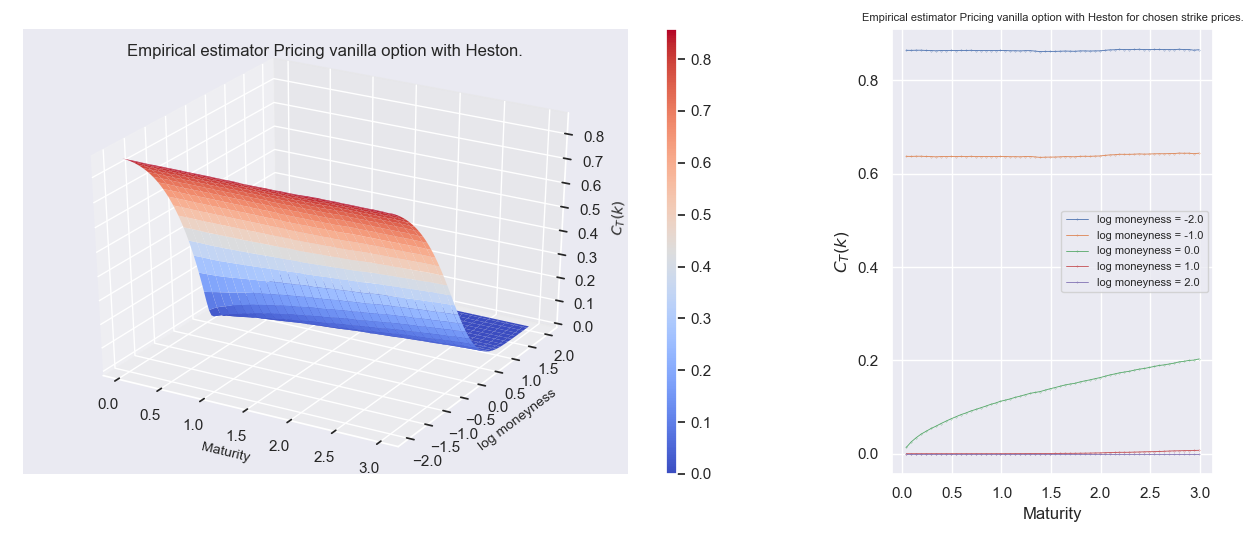
\includegraphics[width = 0.9 \textwidth]{../addition_part/images/integration_fft/empirical_pricing_5000_cover.png}
   \caption{Pricing frontier with the empirical estimator, 20000 simulations.}
   \label{fig:simulations_empirical_pricing_2}
\end{figure}


The theory indicates that the last findings are correct. However, let's verify that by comparing the previous graphs to the one computed under the closed form. We do that in the next section.



\subsection{Closed Form}

As already mentioned, there exists a closed form formula for the characteristic function of an asset whose dynamic is computed with the Heston model. The often used closed form is with a risk premium equal to zero (i.e. the equations (\ref{eq:original_problem1}), (\ref{eq:original_problem2}), (\ref{eq:original_problem3}) reduce respectively, under $\theta = 0$, to (\ref{eq:model1}), (\ref{eq:model2}), (\ref{eq:model3})).

The closed form exists only when the model is markovian or put it differently, when $\alpha = 1$. The considered model (eq. (\ref{eq:model1}), (\ref{eq:model2}), (\ref{eq:model3})), with the trivial kernel, and under the asumption of a null risk premium, reduces to:


\begin{align}
d V_t &= \kappa  (  \phi - V_t ) dt + \sigma \sqrt{V_t} dB_t \\
d S_t &= S_t r_t dt + S_t \sqrt{V_t} d W_{1,t} \\
d B_t &= \rho d W_{1,t} + \sqrt{1- \rho^2 } d W_{2,t} 
\end{align}


Here follows the closed form for the characteristic function $\Phi$, as proposed by Heston in \cite{Heston}:



$\Phi_T(\xi) = \exp\Big(C_T(\xi) + D_T(\xi)V_0 + \mathrm{i}\xi \log(S_0)\Big)$, where
\begin{align*}
C_T(\xi) & := \mathrm{i}r\xi T + \frac{\kappa \phi }{\sigma^2}\left\{\left(\kappa-\mathrm{i}\rho\sigma\xi+d_T(\xi)\right)T
- 2\log\left(\frac{1-\gamma_T(\xi)\mathrm{e}^{d_T(\xi)T}}{1-\gamma_T(\xi)}\right)\right\},\\
D_T(\xi) & := \frac{\kappa - \mathrm{i}\rho\sigma\xi + d_T(\xi)}{\sigma^2}
\left(\frac{1-\mathrm{e}^{d_T(\xi)T}}{1-\gamma_T(\xi)\mathrm{e}^{d_T(\xi)T}}\right),\\
\gamma_T(\xi) & := \frac{\kappa-\rho\sigma - \mathrm{i}\rho\sigma\xi + d_T(\xi)}
{\kappa-\rho\sigma - \mathrm{i}\rho\sigma\xi - d_T(\xi)},
\qquad 
d_T(\xi) := \sqrt{(\kappa-\rho\sigma-\mathrm{i}\rho\sigma\xi)^2 + \sigma^2(\mathrm{i}\xi - \xi^2)}.
\end{align*}

However, it is well known that this characteristic function may have branch-cut issues, for that reason one should instead use the solution proposed in \cite{gatheral} which doesn't suffer from any branch-cut issues. The other preferable expression is the following:


$\Phi_T(\xi) = \exp\Big(C_T(\xi) + D_T(\xi)V_0 + \mathrm{i}\xi \log(S_0)\Big)$, where
\begin{align*}
C_T(\xi) & := \mathrm{i}r\xi T + \frac{\kappa\phi}{\sigma^2}\left\{\left(\kappa-\mathrm{i}\rho\sigma\xi-d_T(\xi)\right)T
- 2\log\left(\frac{1-\gamma_T(\xi)\mathrm{e}^{-d_T(\xi)T}}{1-\gamma_T(\xi)}\right)\right\},\\
D_T(\xi) & := \frac{\kappa - \mathrm{i}\rho\sigma\xi - d_T(\xi)}{\sigma^2}
\left(\frac{1-\mathrm{e}^{-d_T(\xi)T}}{1-\gamma_T(\xi)\mathrm{e}^{-d_T(\xi)T}}\right),\\
\gamma_T(\xi) & := \frac{\kappa - \mathrm{i}\rho\sigma\xi - d_T(\xi)}{\kappa - \mathrm{i}\rho\sigma\xi + d_T(\xi)},
\qquad 
d_T(\xi) := \sqrt{(\kappa-\mathrm{i}\rho\sigma\xi)^2 + \sigma^2(\mathrm{i}\xi+\xi^2)}.
\end{align*}

This is the form we will use through the paper. First the integrands are visible there fig. \ref{fig:integrands_closedform}. We recall that the domain of integration can be chosen manually in order to reduce integration errors. My strategy was to observe the integrands for a few strike prices, and pick the max where the function is non zero. Then to this value I add some leeway, in case I wasn't exactly accurate.

Additionally, the pricing under the parameters from table  \ref{table:parameters_for_closed_form} can be seen in fig. \ref{fig:price_closed1} and in fig.
\ref{fig:price_closed2}.

\begin{figure}
\centering
   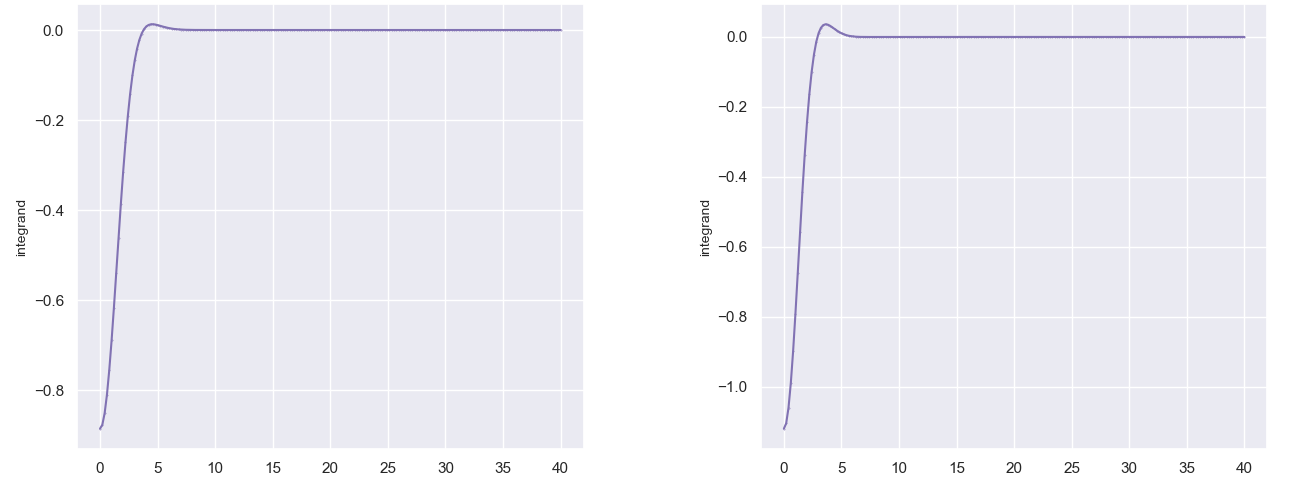
\includegraphics[width = 0.9 \textwidth]{../addition_part/images/integration_fft/closed_form_integrands.png}
	\caption{Integrands for (\ref{eq:Pis}) with the closed form, where the observed log strike price is equal to one. $\Pi_1$ on the left, $\Pi_2$ on the right. First set of parameter, from \ref{table:parameters_for_closed_form}.}
   \label{fig:integrands_closedform}
\end{figure}


\begin{figure}
\centering
   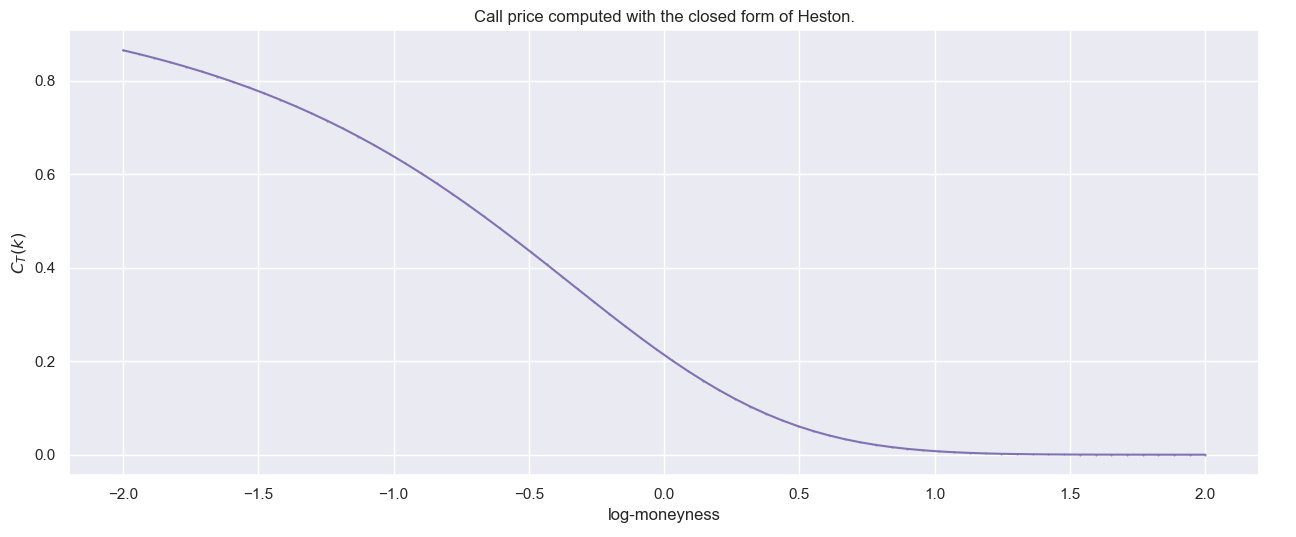
\includegraphics[width = 0.8 \textwidth]{../addition_part/images/integration_fft/pricing_closed_form_heston.png}
   \caption{Option's price with Heston, exact computation, first set of parameters, from \ref{table:parameters_for_closed_form}.}
   \label{fig:price_closed1}
\end{figure}


\begin{figure}
\centering
   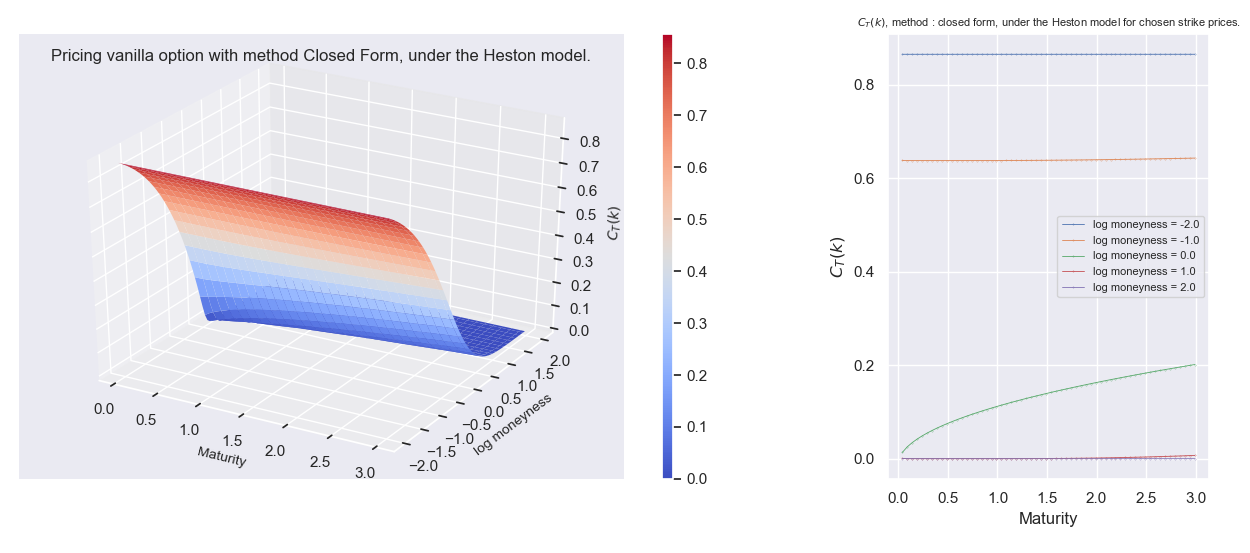
\includegraphics[width = 0.9 \textwidth]{../addition_part/images/integration_fft/closed_form_pricing_surface&few_Heston.png}
   \caption{Exact Pricing Frontier for an option with Heston, first set of parameters, from \ref{table:parameters_for_closed_form}.}
   \label{fig:price_closed2}
\end{figure}




\subsection{Discussion of the results}
\label{comparaison_integrands}
One shall notice that the figures \ref{fig:integrand_kde}, \ref{fig:integrand_moments} and \ref{fig:integrands_closedform}, which are the figures for the three methods of computing the characteristic functions, yield different results. The worst one comes from the usage of moments. One can observe that the method is really unstable. Same observation for the characteristic function using KDE, which is negative for strike prices between 0.5 and 2.
\label{comparaison_price}
Therefore, the two first incorrect methods are definitely wrong, as prices were negative and far from the truth. Also, the complexity cost for computing those estimates was very high.

Finally, with no surprise, the empirical pricing (section \ref{empirical_price}) was correct and it totally agrees with the closed formula, as one can see that both curves are identical: fig. \ref{fig:simulations_empirical_pricing} and fig. \ref{fig:price_closed1}.


To conclude this section, one can see the results under a different set of parameters in fig. \ref{fig:new_param} and in fig. \ref{fig:new_param2}. We also compare it to the empirical pricing in fig. \ref{fig:new_param_estim} and in fig. \ref{fig:new_param2_estim}. The results confirm that the empirical method is working properly.


\begin{table}
\begin{center}
\begin{tabular}{   m{4.5 cm} | m{4.5 cm} | m{4.5 cm}   } 
\hline
 Parameter & Set $1$ & Set$ 2$ \\ 
\hline
\hline
$V_0$ & $0.1$ & $0.1$ \\
\hline
$S_0$ & $1$ & $1$ \\
\hline
$r$ & $0$ & $0.2$ \\
\hline
$\sigma$ & $0.1$ & $0.3$ \\
\hline
$\rho$ &$ -0.56$ &  $-0.56$\\
\hline
$\theta$  &  $0.0$ &$ 0.0$ \\
\hline
$\kappa$ & $1$ & $1$ \\
\hline
$\phi$ & $0.1$ &  $0.1$ \\
\hline
$T$ & $3$ &  $3$ \\
\hline
\end{tabular}
\caption{The two different sets of parameters.}
\label{table:parameters_for_closed_form}
\end{center}
\end{table}


\begin{figure}
\centering
   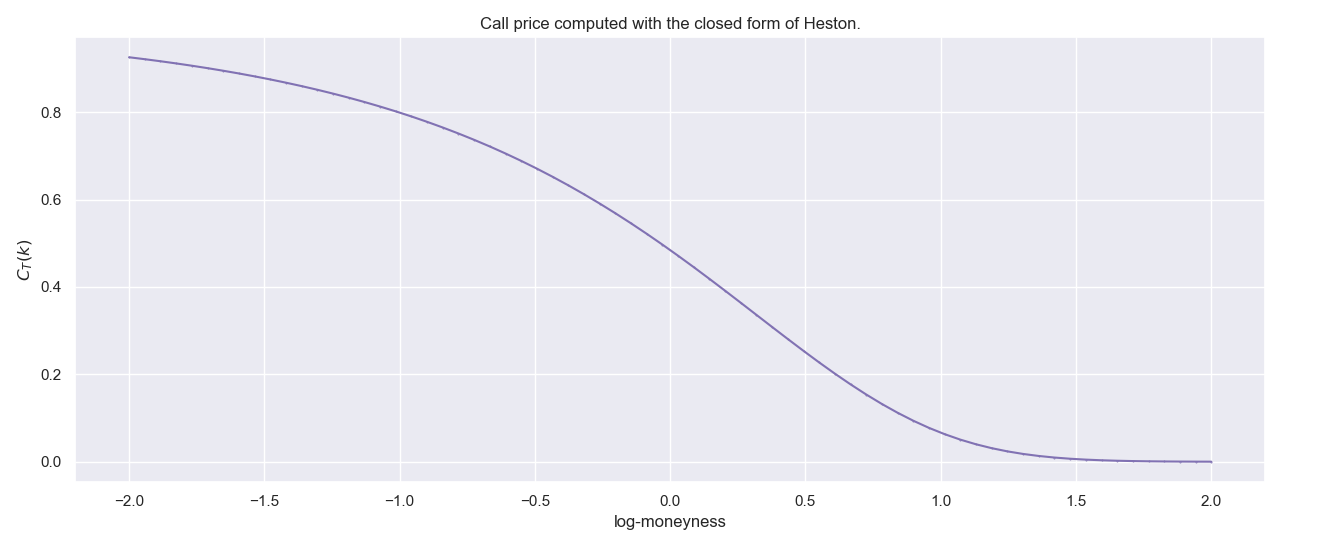
\includegraphics[width = 0.75 \textwidth]{../addition_part/images/integration_fft/closed_price_1_new.png}
   \caption{Exact Price for an option with Heston, second set of parameters, from \ref{table:parameters_for_closed_form}.}
   \label{fig:new_param}
\end{figure}

\begin{figure}
\centering
   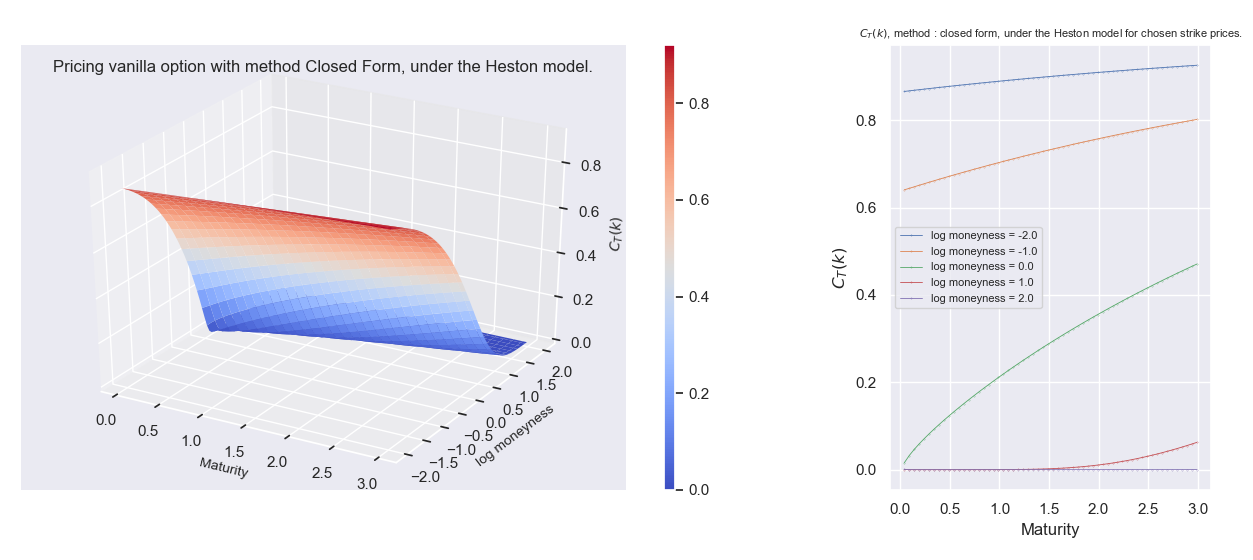
\includegraphics[width = 0.9 \textwidth]{../addition_part/images/integration_fft/closed_price_1000_new.png}
   \caption{Exact Pricing Frontier for an option under the Heston Model, second set of parameters, from \ref{table:parameters_for_closed_form}.}
   \label{fig:new_param2}
\end{figure}


\begin{figure}
\centering
   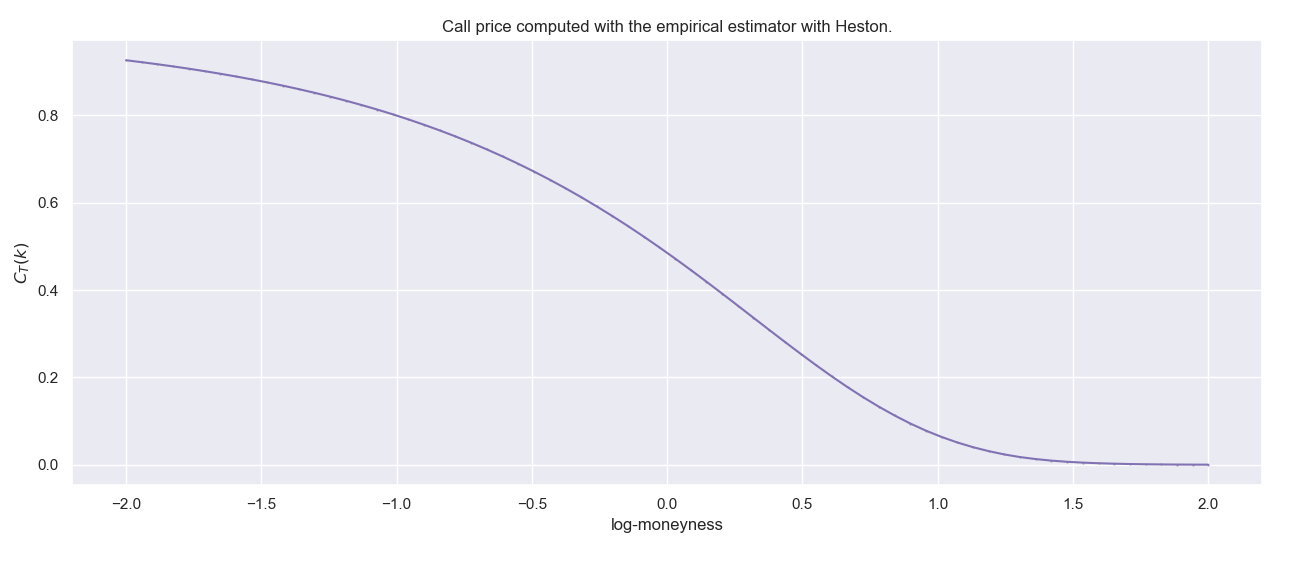
\includegraphics[width = 0.75 \textwidth]{../addition_part/images/integration_fft/empirical_pricing_5000_new.png}
   \caption{Empirical Price for an option with Heston, second set of parameters, from \ref{table:parameters_for_closed_form}.}
   \label{fig:new_param_estim}
\end{figure}

\begin{figure}
\centering
   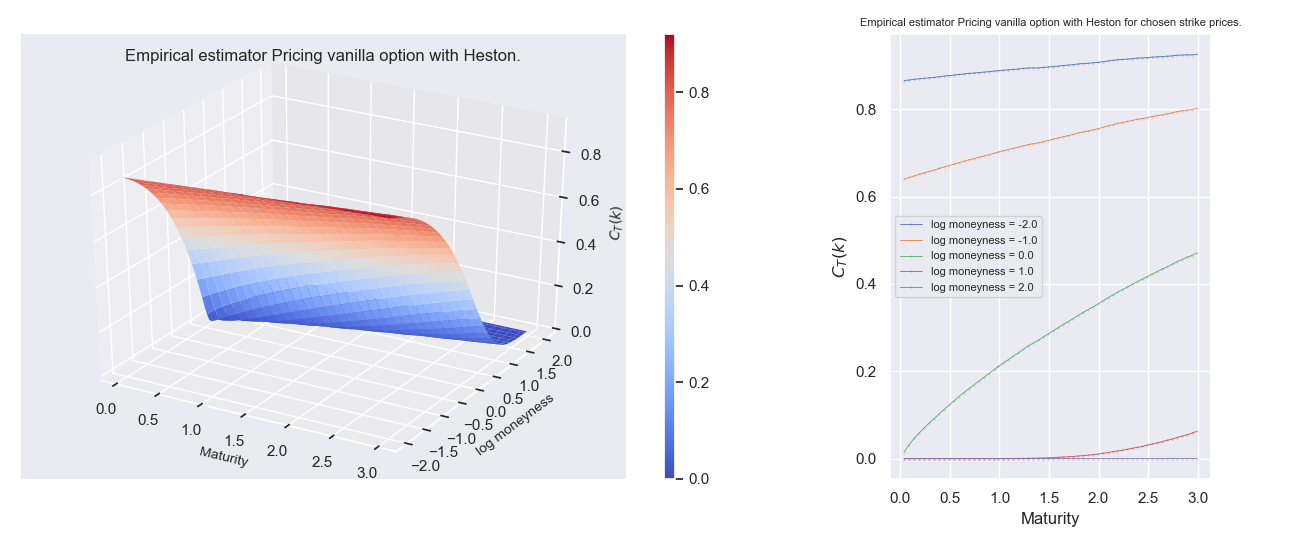
\includegraphics[width = 0.9 \textwidth]{../addition_part/images/integration_fft/empirical_pricing_5000_cover_new.png}
   \caption{Empirical Price frontier for an option with Heston, second set of parameters, from \ref{table:parameters_for_closed_form}.}
   \label{fig:new_param2_estim}
\end{figure}

\subsection{Comparison Empirical / Closed form with the Implied Volatility}

Comparing prices is in fact not enough in order to compare models. It can be inaccurate because what is interesting is not only the price itself, but also the shape of the curve. Two prices can be very close on the graph, and could come from two totally different models. This is especially true for far from the money prices. Then, a better way to compare pricing is using the implied volatility. 

We do that in the relevant section (cf. section \ref{section:IVempirical}), after the introduction of the concept of implied volatility. Also, another thing that could be interesting to do, is checking how fast the empirical estimator converges toward the true pricing. We do that with the help of the IV later on, in the same section.

\subsection{Calibration to Market Prices}
Finally, once the formulas are working, one could try to find the parameters to fit the models to the markets and use pricing models to trade. This step is called calibration to market prices.

I haven't studied it much, this might be a good thing to study as a further step, and for now I simply give the reference to this paper: \cite{ricardo} and to this stackexchange question: 
\begin{Verbatim}[fontsize = \tiny]
https://quant.stackexchange.com/questions/18400/option-pricing-model-calibration-in-practice
\end{Verbatim}







\section{Faster Option Pricing with FFT}
\subsection{Theory}

Developed by Peter Carr and Dilip Madan in the paper \cite{CarrMadan}, there is a method that takes advantage of the Fast Fourier Transform algorithm to increase the speed of the previously presented pricing methods. The original computation should require $o(n^2)$ operation, and using the FFT algorithm reduces it to the possible minimum: $o(n \log_2(n)) $.

First, they wrote the pricing formula in the following way, involving only one integral. Back from (\ref{eq:super_pricing}):

$$ C_T(k) = e^{-rT } \E_{\mathbb Q} ( (S_T - K)^+ ) = e^{-rT } \int_k^{\infty} (e^x - e^k) q_T (x) dx $$

where recall that $k := \ln (K)$ and $q_T$ is the distribution of the log price of the asset.

Then, they took advantage of the particular form of the Fourier transform of $C_T(k)$.

We want to take the Fourier transform of $C_T(k)$:$$\tilde{\psi}(\xi) := \int_{\mathbb  R} e^{i \xi k } C_T(k) dk  $$

Notice that the function is constant at the limit: 
$C_T(k) \xrightarrow[k \to -\infty]{} S_0$, as a result there is a problem of integrability of that function\footnote{Hence, its Fourier transform does not exist}. This leads to a singularity in the characteristic function at $0$; Accordingly, the Fourier transform of the payoff function has large high-frequency term.  The solution proposed by Carr and Madan is to multiply the expression by a strictly positive constant (called $\alpha$) that would dampen the expression and make it integrable, then lowering the importance of the singularity at the cost of the degradation of the solution. This technique is not new, someone already proposed it in the fifties. One shall be careful with the choice of the damping constant. We want the price to be integrable ($ C_T(k) \in L^1$) and we also want its Fourier transform to be integrable ($\psi \in L^1$) in order to take back the price. 

We will detail the choice of $\alpha$ later.

Thus we define a new pricing function in the following way
\begin{align} \label{eq:dampened}
C_T(k) &= e^{- \alpha k} e^{ \alpha k } C_T(k) \nonumber \\ 
&=: e^{- \alpha k} c_T(k)
\end{align}

Coining: $ \psi(\xi) := \int_{\mathbb  R} e^{i \xi k } c_T(k) dk  $, we have from (\ref{eq:dampened}): 

\begin{align} \label{eq:price}
C_T(k) &= \frac{ e^{- \alpha k }} { 2 \pi } \int_{\mathbb R} e^{-i \xi k } \psi( \xi ) d \xi \nonumber \\
&= \frac{ e^{- \alpha k }} {  \pi } \int_0^{\infty} e^{-i \xi k } \psi( \xi ) d \xi 
\end{align}

where we used in the second line symmetry properties of the integrand. The justification can either be found in \cite{CarrMadan}, where they said that since $C_T(k)$ is real (by definition), $ \psi $ is hermitian (cf. following theorem for the general statement), or one can notice that $\psi$ conserves the hermitian property of $\phi_T$. 

\begin{theoreme}{Decomposition of a Fourier transform}
Writing: $\hat{f}$ as the Fourier transform of $f$, then, using the unique even/odd decomposition for functions (denoted here with the subscript Even and Odd):

$$ 
\hat{f}(\xi) = \frac{1}{2 \pi } \int_{\mathbb R} f_e(x) cos(\xi x)  dx  - \frac{i}{2 \pi } \int_{\mathbb R} f_o(x) sin(\xi x)  dx 
$$

$$ 
f(x) =  \int_{\mathbb R} \hat{f_e}(\xi) cos(\xi x)  dx  + i \int_{\mathbb R} \hat{f_o}(\xi) sin(\xi x)  dx 
$$

Thus, if $f$ is real, then $\hat{f}$ is hermitian, and if $\hat{f}$ is real, then $f$ is hermitian.

\end{theoreme}

Also, one can prove that $\psi$ admits a closed form as a function of the characteristic function $\phi_T$:

\begin{equation} \label{eq:psi}
 \psi (\xi ) = e^{-rT} \frac{ \phi_T ( \xi - i ( \alpha + 1 ) ) }{( \alpha + i \xi )(1 + \alpha + i \xi )} 
\end{equation}

Therefore, when the characteristic function admits a closed form, $\psi$ also admits a closed form. Finally, $C_T(k)$ can be priced using the FFT algorithm on $\psi$ (using (\ref{eq:psi}) in (\ref{eq:price})). We will discuss the process in section \ref{method-fft}.

\subsection{Difficulties and choice of $\alpha$}
\begin{itemize}


\item One notices that in (\ref{eq:psi}), if $\alpha = 0$, the denominator vanishes when $ \xi =0$, inducing a singularity in the integrand.

\item $\alpha$ should be chosen in order to have integrability. $\alpha$ should be bigger than $0$. On the other side, if $\alpha$ is too big, the Fourier transform wouldn't be integrable. From previous numerical experience,  $\alpha = 1$ works well for the considered model of asset price dynamics. Roger Lee recommends \cite{roger_lee} this upper bound: 

$$ \alpha_+ := \sup \{ \alpha  > 0 : \mathbb E_{\mathbb Q} ( S_T^{\alpha + 1} )  < \infty  \} $$ 

On the other hand, why not choose an $\alpha$ really close to 0? The problem with a small $\alpha$ is that it alters the final results. Even thought it doesn't change the theoretical expression, it could potentially slightly change the numerical results. For that reason, one should take the biggest $\alpha$ possible.

\item At the end, it is important to observe that $\alpha$ has to be chosen such that the denominator has only imaginary roots, since we are integrating over the positive real values. 


\item Put options can be price similarly taking a negative $\alpha$ for obvious reasons of integrability. Finally, it is possible to extend those properties to general options, but that bit of theory is not described here and I recommend anyone interested in that to look at \cite{num_methods} in particular to theorem $4.2.3$ in the lecture notes.


\item One of the drawbacks of the algorithm is that however, as have already noticed Carr and Madan in \cite{CarrMadan}, (\ref{eq:psi}) is highly oscillatory and difficult to integrate numerically for strike prices far from the ATM level and for short maturities. This causes significant numerical errors. One shall look into \cite{fft_improve} where one method to reduce that error is proposed.

\item Another flaw is that one can't have the exact prices for every single strike he desires, since the FFT algorithm forces a grid of strike prices. Hence, when this algorithm is used, an additional interpolation error is added. In parallel, the more precise one wants to get, the more expensive it is. The algorithm prices options further from ATM. One thing I did in the following is using the FFT for a large number of strike prices, and then zooming around ATM prices.

\end{itemize}


For those craving for more details, the excellent (but technical) paper \cite{optimal_fourier_inversion} will do the trick.

Another interesting approach would be the cosine method, topic I haven't studied. Readers are invited to check \cite{num_methods} page $145$, and the original paper: \cite{fang}.


\subsection{Method}
\label{method-fft}

We skip details about how the FFT works, though one could refer to \cite{annalisa} or to \cite{num_methods} for more information about Fourier transforms and FFT algorithm. Also, \cite{fft_improve} offers a clear explanation of the algorithm as well as some applications to different original types of option pricing models and payoffs as for instance Bermudan style options under Levy processes.



To put it short, the FFT algorithm is an efficient algorithm to compute sums of the following form: 

\begin{equation}
\label{eq:FFT_form}
F_k = \sum_{j=0}^{n-1} \exp \left ( - i \frac{ 2 \pi }{ n } j k \right ) f(j) \text{,} \quad \text{ for } k \in \{ 0, \cdots n-1 \} 
\end{equation}

where the number of nodes $n$ is a power of $2$ for computing efficiency. As mentioned, it reduces drastically the complexity of the computation.

In order to apply the FFT algorithm to our equation (\ref{eq:price}), we first discretize the expression using Simpson's rule. We need to define a grid for the evaluation. On the strike size, we define a grid with $\lambda_{step}$ as step. Our choice is a regular symmetric grid around the origin, of length $n$, which will give us the prices at those log strike prices:

$$ k_u =  - \lambda_{step} \frac { n } 2 + \lambda_{step} u, \quad \text{ for } u \in \{ 0, \cdots, n-1 \} $$

graphically :


\begin{figure}[h]
\centering
\begin{tikzpicture}
\foreach \x/\y in {
-6.2/ k_{0} = - \lambda_{step} \frac { n } { 2 } , 
-4.4/ k_{1},
0.6/ k_{ \frac{n}{2} + 1} = \lambda_{step} , 
-1.6/ k_{ \frac{n}{2}} = 0, 
3.2/ k_{n - 2}, 
6/ k_{n-1} =   \lambda_{step} (\frac { n } { 2 } - 1 )      }
 \draw[thick] (\x,0.2) -- (\x,-0.2) node[below]{$\y$};
\draw[thin] (-3,-0.10)--(-2.8 ,0.10);
\draw[thin] (-3.1,-0.10)--(-2.9 ,0.10);
\draw[thin] (1.9,-0.10)--(2.1 ,0.10);
\draw[thin] (2,-0.10)--(2.2 ,0.10);
\draw[thin] (-7.5,0)--(7.5 ,0);
\end{tikzpicture}
\end{figure}


parallelly, the frequencies where we evaluate the characteristic function are defined with another grid. Increasing the number of frequency points increases the precision of each price. We use a regular frequency-grid, with step $\eta_{step}$ yielding: $ \xi_j =j \cdot  \eta_{step}$, for $j \in \{ 0, \cdots, n-1 \} $. Now we can approximate the call price:


\begin{align}
C_T(k_u) &= \frac{ e^{- \alpha k_u }} {  \pi } \int_0^{\infty} e^{-i \xi k_u } \psi( \xi ) d \xi  \nonumber \\
& \approx \frac{ e^{- \alpha k_u }} {  \pi } \int_0^{ n \eta } e^{-i \xi k_u } \psi( \xi ) d \xi   \label{eq:truncation} \\
&\approx \frac{ e^{- \alpha k_u }} {  \pi } \sum_{j=0}^{n-1} 
a_j \exp \left ( - i k_u \xi_j \right )  \psi(\xi_j)   \label{eq:discrete} \\
& =  \frac{ e^{- \alpha k_u }} {  \pi } \sum_{j=0}^{n-1} 
a_j \exp \left ( 
i \cdot ( \lambda \frac n 2 - \lambda u ) \cdot \eta j 
\right )  \psi(\xi_j) 
\label{eq:final_form_pricing}
\end{align}

where the $a_j$ are the weights in the quadrature. With the composite Simpson's rule:

$$
a_j = \left\{
    \begin{array}{lll}
        \frac{ \eta_{step} } 3 & \mbox{if } j \in \{0,n-1 \}  \\
        4 \frac{  \eta_{step} } 3 & \mbox{elif } j \equiv 1 \;(\bmod\; 2) \\
        2 \frac{ \eta_{step} } 3 & \mbox{elif } j \equiv 0 \;(\bmod\; 2) \\
    \end{array}
\right.
$$

The last step, in order to apply the FFT algorithm, we apply a condition on the product $ \eta \lambda $, making the identification between (\ref{eq:FFT_form}) and (\ref{eq:final_form_pricing}) possible. This fixes: $ \lambda \eta = \frac {2 \pi } n $. Then, the final scheme looks like:

\begin{theoreme}{Pricing with the FFT and a closed form formula }
\begin{equation}
\label{eq:final_form_pricing_final}
C_T(k_u) = \frac{ e^{- \alpha k_u }} {  \pi } \sum_{j=0}^{n-1} 
a_j \exp \left ( 
- i \cdot \frac{2 \pi} {n} \cdot  u  \cdot   j 
\right ) 
e^{ i \pi  j }
\psi(\xi_j) 
\end{equation}
\end{theoreme}

A quick word about the introduced errors. The first error introduced in (\ref{eq:truncation}) is called a truncation error. It comes from the fact that the effective upper limit for the integration became, by truncation, $[0, n \eta ]$. Additionally, the integral is sampled in (\ref{eq:discrete}) for quadrature and results a sampling error. Intuitively, I would say that this error should be nicely bounded because we used the Simpson's method whose error is in $o( \frac 1 {n^4})$. However, we also saw that the function is highly oscillatory near $0$, then the bound upon the error might not be accurate. A more rigorous discussion of the error can be found in \cite{roger_lee}.





\subsection{Results}


The results are presented in the following figures: fig. \ref{fig:fft}.

The graph only shows prices near ATM. What happens is that one observes explosions for prices out of the money, due to the errors previously mentioned. Nevertheless, increasing the precision near the money comes with having prices out of the money, so zooming is a must. One notices that the prices are slightly scaled, but the shape corresponds. In order to check if the shape corresponds, I computed the ratio between the price given by the FFT and the price given by the close form formula. I plotted the ratios in fig. \ref{fig:fft_ratio}. It is clear that the ratio is not constant, however, for prices OTM and ATM, where also the price is not closed to zero, the ratio remains relatively constant ($[1.35,2]$), or at least, constant in a small neighbourhood. The ratio explodes in particular to prices far in the money, where the pricing is close to zero everywhere. It looks exponential for prices ITM.

Then, one can say the pricing is accurate, even though it has to be rescaled.


\begin{figure}
\centering
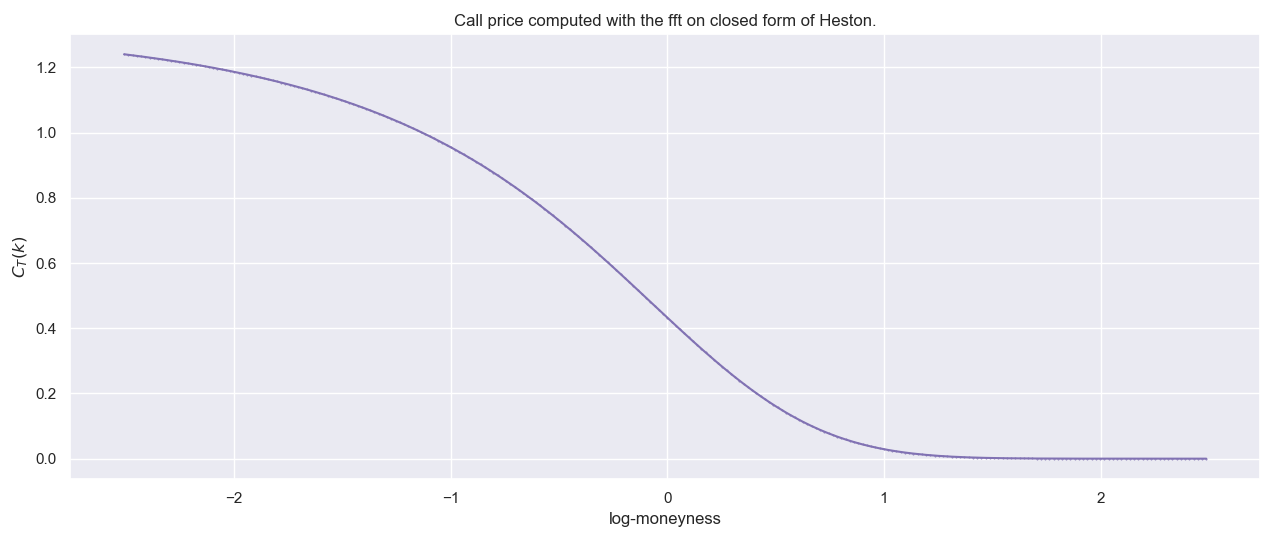
\includegraphics[width = 0.7 \textwidth]{../addition_part/images/integration_fft/fft.png}
\caption{Results of pricing with FFT.}
\label{fig:fft}
\end{figure}


\begin{figure}
\centering
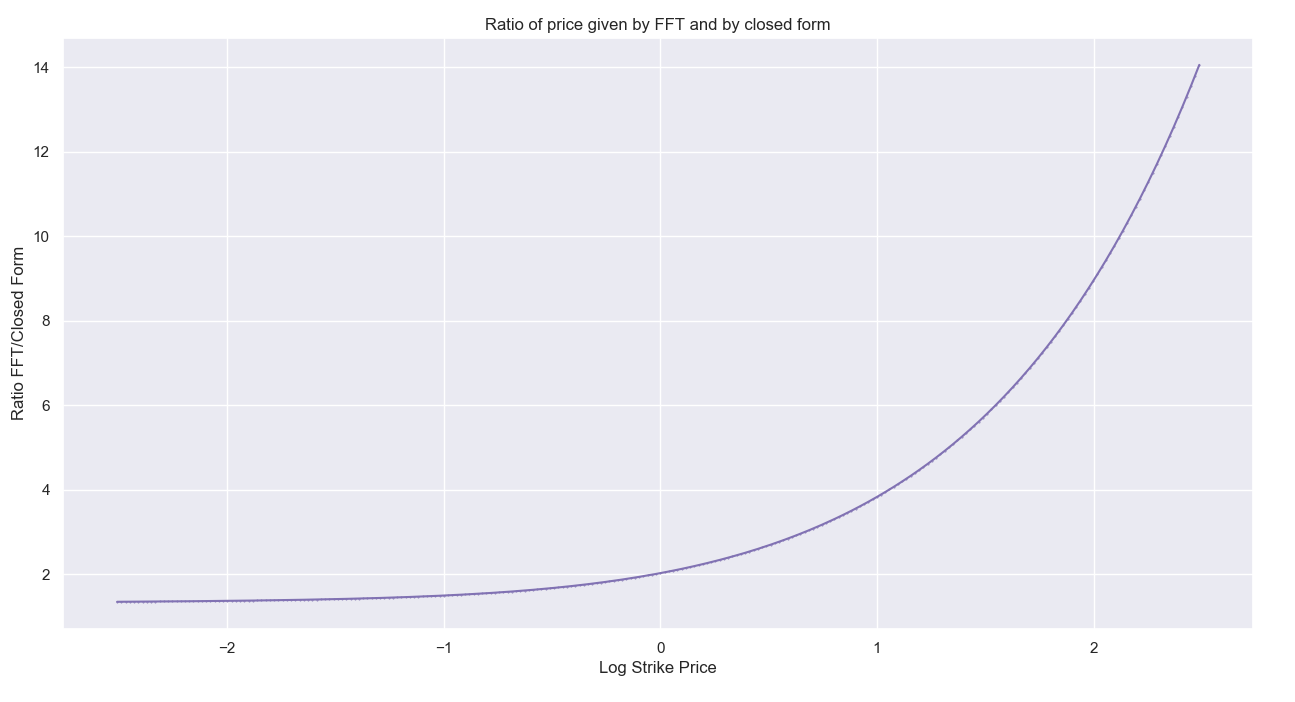
\includegraphics[width = 0.7 \textwidth]{../addition_part/images/integration_fft/fft_ratio.png}
\caption{Verification of the pricing by FFT.}
\label{fig:fft_ratio}
\end{figure}





















\section{Implied Volatility}
\subsection{Definition}

\begin{definition}[Implied Volatility]

The implied volatility is a metric that captures the market's view of the likelihood of changes in a given security's price. 

It is deeply connected to the B$\&$S formula. 

Still in a philosophical way, the implied volatility is the volatility of the model if it was computed under the Black and Scholes model. As a result, estimating the IV allows to estimate how volatile a model is in comparison to a standard model. Then, if the former is riskier (resp. less), the premium for options should be higher (resp. lower). 

Mathematically, the B$\&$S formula can be inverted (cf. theorem \ref{thrm:BSformula} and appendix \ref{anx:invert_BS}). The implied volatility $ \sigma_{IV} $ is defined as the unique positive solution of:
\begin{equation}
\label{eq:IVunique}
C_{BS} ( S_0, K, T, \sigma_{IV} ) = C ( S_0, K, T )
\end{equation}

Then, IV helps us understand how the market estimates the volatility of a stock.

\end{definition}


One can see in fig. \ref{fig:BSvolatilitymaxcase} an example of the prices of the Heston model stuck between the two extreme cases of the Black and Scholes model (which corresponds to the extreme cases where the volatility has been taken to extremely high and low variance). Then, finding the $\sigma_{IV}$ that solves the equation is reduced to a root-finding problem.

One way to find the root is by using numerical efficient algorithms. The first one used is the bissect algorithm. Also, later, we test the efficiency of the Newton-Raphson algorithm.
\subsection{Implied Volatility for B$\&$S}
\begin{figure}
\centering
\subfloat{{
\includegraphics[width = 0.6 \textwidth]{../addition_part/images/BS/BSIV2.png}
}}\\
\subfloat{{
\includegraphics[width = 0.6 \textwidth]{../addition_part/images/BS/BSIV1.png}
}}\\
\subfloat{{
\includegraphics[width = 0.6 \textwidth]{../addition_part/images/BS/BSIV3.png}
}}\\
\caption{IV for B$\&$S in the case (parameters of B$\&$S: $r = 0, X_0 = 1$) of $\sigma = 0.03, 0.1, 0.3$.}
\label{BSIVflat}
\end{figure}

As one can expect from the definition, the IV for B$\&$S model should be flat. It is indeed flat to the extent of numerical errors, especially for strike prices far from ATM (cf. fig. \ref{BSIVflat}). Usually, the interesting strike prices are around $0$ on a range of 10$\%$. In other words, the flatness of the curve for the Black and Scholes model is verified. Also, one notices that the higher the variance, the less is the implied volatility influenced by large far ATM strike prices. This is explained by the fact that a greater volatility allows more flexibility for the convergence of the iterative algorithms. One can read section  \ref{diff_vega} for more details.

\subsection{Implied Volatility for Empirical pricing}
\label{section:IVempirical}
Fig. \ref{fig:IVempirical} shows the implied volatility of the pricing estimator. We use the same parameters as before (table \ref{table:parameters_for_closed_form}).

\begin{figure}
\centering
\includegraphics[width = 0.7 \textwidth]{../addition_part/images/integration_fft/IVempirical.png}
\caption{Implied Volatility of the empirical pricing for 5000 simulations. Closed form in red, empirical in purple. First set of parameters, from table \ref{table:parameters_for_closed_form}. }
\label{fig:IVempirical}
\end{figure}

The IV is pretty similar to the closed form one, which are respectively represented by the purple line and red dotted line. One can see that the IV gets to $0$ for log strikes prices higher than $1.8$. This is due to numerical errors. Also, one observes that the shape of the empirical IV gets further from the closed form's one as strike prices get more extreme. This is due to the fact that the estimator hasn't fully converged yet. So one can say that the empirical pricing is a good estimator of the price. Nevertheless, its precision decreases as one gets further from ATM prices.

Now, we change the parameters, and we plot again the empirical implied volatility. It is visible on fig. \ref{fig:IVempirical2}. We observe the same good behaviour of the estimator, confirming that the natural empirical estimator works correctly to estimate the price.

\begin{figure}
\centering
\includegraphics[width = 0.7 \textwidth]{../addition_part/images/integration_fft/IVempirical2.png}
\caption{Implied Volatility of the empirical pricing for 5000 simulations. Closed form in red, empirical in purple. Second set of parameters, from table \ref{table:parameters_for_closed_form}. }
\label{fig:IVempirical2}
\end{figure}

Finally, we want to see the impact of the number of random paths generated on the convergence of the estimator. One way to do it would be to compute the MSE of the estimator in order to check the consistency\footnote{Consistency follows from MSE convergence, cf. \cite{panaretos}.}. In order to not delve into too much details, we do a simple heuristic comparison.

With fig. \ref{fig:IVempirical_evol}, we plot the convergence of the estimator, in implied volatility scale, with respect to the number of random paths generated. We observe that more simulations increase the precision: the highest simulated number, represented by the purple shape, is closer to the dotted line, the latter corresponding to the true implied volatility. However, we see that when one goes further from ATM, the shape diverges. In fact, on the right (far ITM), the IV is constantly zero; on the left (far OTM), the IV is not computable anymore as the values are not invertible anymore.

An interesting thing to notice is that even though the prices are indeed all very close to the true price (left graph), the IV shapes are all different. Hence, the IV is a better indicator of convergence of the empirical estimator. However, it is also very sensible as one can see in fig. \ref{fig:IVempirical_evol2}. In the second graph, we plotted the same estimator, under the same parameters but for a number of simulations much higher. Now we observe that the estimator with the most simulations (60000 paths generated) is very far from the true IV. My rational for this phenomenon is that the estimator converged to the true price, modulo a numerical error, that stacks up as the number of simulations increases.

\begin{figure}
\centering
\includegraphics[width = 0.95 \textwidth]{../addition_part/images/integration_fft/low_IV_empirical.png}
\caption{Evolution of the empirical implied volatility for small amount of simulations. True IV in black. Parameters same as for \ref{fig:IVempirical_evol2}.}
\label{fig:IVempirical_evol}
\end{figure}


\begin{figure}
\centering
\includegraphics[width = 0.95 \textwidth]{../addition_part/images/integration_fft/high_IV_empirical.png}
\caption{Evolution of the empirical implied volatility for large number of simulations. True IV in black. Parameters of the simulation at the bottom of the image.}
\label{fig:IVempirical_evol2}
\end{figure}



\subsection{Computation}
The computation is given by that function, and fig. \ref{fig:iv_bissect} shows the result for a change of the vol of vol under the Heston model. We will shortly compare that graph to the one obtained from another method of root-finding.

\begin{verbatim}
def implied_volatility_empirical_heston(S, k, s0, T, R):
    ## s0 starting point of the S's,
    ## S realisation of the S_T
    my_price = empirical_price_option(S, k, T, R)

    def smile_min(vol, *args):
        k, s0, T, r, price = args
        return price - BlackScholes(True, s0, k, T, r, 0., vol)

    vMin = 0.000001
    vMax = 10.
    # in order to find the implied volatility, one has to 
    # find the value at which smile_min crosses zero. 
    return scipy.optimize.bisect(smile_min, vMin, vMax, 
    args=(k, s0, T, R, my_price), xtol=1e-20, rtol=1e-15,
    full_output=False, disp=True)
\end{verbatim}


\begin{figure}
\centering
   \includegraphics[width = 0.75 \textwidth]{../addition_part/images/integration_fft/Heston_IV.png}
   \caption{Implied volatility computed with bissect method.}
   \label{fig:iv_bissect}
\end{figure}











\subsection{Newton Raphson}
Another way to solve the implied volatility equation  (\ref{eq:IVunique}) is the Newton-Raphson. It is an efficient iterative algorithm to find the roots of a function, while using its derivative.

For more details about theory and convergence, I redirect anyone to the lecture notes of Albina Danilova: "Optimization with Applications in Portfolio Choice" (LSE). The main idea in Newton-Raphson algorithm lays upon the following equation:

$$ \sigma^{ \text{imp} }_{k+1} = \sigma^{ \text{imp} }_{k} - \frac{f\sigma^{ \text{imp} }_{k})}{  f'(\sigma^{ \text{imp} }_{k})} $$

or written equivalently, we are searching for the solution to the equation: 

$$ f(\sigma^{ \text{imp} }_{k}) + f'(\sigma^{ \text{imp} }_{k}) \cdot (\sigma^{ \text{imp} }_{k+1} -\sigma^{ \text{imp} }_{k} ) = 0 $$
Starting with an initial guess, the approximate solutions iteratively improve until a certain criterion is satisfied. The function $f$ and its derivative are given by the following. The latter is also referred to as "Vega". The computation of those formulas can be found in \ref{anx:invert_BS}.

\begin{align*}
f(x) &= C_{BS} - C_{Heston} \\
f'(x) &= \text{ VEGA } (C_{BS}) = S_0 N'(d_+)\sqrt{T}
\end{align*}



\begin{figure}
\centering
   \includegraphics[width = 0.75 \textwidth]{../addition_part/images/integration_fft/Heston_NEWTON_IV.png}
   \caption{Implied volatility computed with Newton Raphson method.}
   \label{fig:iv_newton}
\end{figure}

\begin{figure}
\centering
   \includegraphics[width = 0.75 \textwidth]{../addition_part/images/integration_fft/Implied_vol_heston_recommandation.png}
   \caption{Optimal $\sigma$ according to Brenner and Subrahmanyan in \cite{Brenner}.}
   \label{fig:brenner}
\end{figure}


A recommendation from \cite{Brenner} about the starting point in Newton-Raphson algorithm applied to the implied volatility is:
$$
   \sigma \approx \sqrt{\cfrac{2\pi}{T}} . \cfrac{C}{S}
$$

where $C$ is the price of the option with respect to the BS model, and $S$ is the spot price. 

It seemed to be a good starting point for options near the money. 
However, it didn't seem to be very conclusive far from ATM. In order to understand why, I plotted the previous equation as a function of the strike price. One can observe that this first guess reduces to zero extremely quickly (cf. fig. \ref{fig:brenner}). It makes this first guess not useful for values far from ATM. Also, under three different $\sigma$ for the model, the shapes of the guess were all relatively very close.

One can see the results of the searching algorithm used for computing the implied volatility in fig. \ref{fig:iv_newton}. It yields the same results (cf. fig. \ref{fig:iv_bissect}) and it seems that using Newton-Raphson takes as much time as to use the implemented method bisect. This must come from the fact that my function is not optimized. The code for Newton-Raphson is on appendix \ref{appendix_code:newton}.

\subsection{Difficulties}
\label{diff_vega}

The principal concern while using root finding algorithms is the failure of convergence. Bissect as well as Newton-Raphson method may fail to converge. Especially, when Vega is extremely small, making the function flat and leading to the stall of the convergence. One notices that the inversion giving the solution is a map from an unbounded interval to a finite one ( $\sigma \in [0, + \infty[ \to [0, S_0 - K e^{-rT} ]$ ). As a result, certain $\sigma-$regions are totally flat and Vega is really close to zero. This happens when the option is either far ITM or OTM. This is visible on fig. \ref{fig:vegabs}.

\subsection{Interpretation}

The typically observed implied volatility shapes in the market, for instance smile or skew, can be obtained by varying the parameters. 

Fig. \ref{fig:diff_sets_param} shows how parameters influence the shape of the implied volatility. The dotted lines have greater $\sigma$, the purple lines are references, the cyan lines have higher $\phi$ and the red ones opposed $\rho$. 

Then, we observe that $\sigma$ is proportional to a sharper curve (the kurtosis), $\phi$ shifts the implied volatility higher and $\rho$ shifts the IV in the more extreme moneyness direction (asymmetry).

\begin{figure}
\centering
   \includegraphics[width = 0.9 \textwidth]{../addition_part/images/integration_fft/comparaison_IV.png}
   \caption{Implied volatility for Heston with different parameters in order to observe their influence.}
   \label{fig:diff_sets_param}
\end{figure}






\section{Option Pricing using a Neural Network}
As personal work, I tried to price options using an artificial neural network (ANN). The target is the well-known B-S model.


\subsection{Data-set}

I generated a data-set randomly with this scheme (cf. table: \ref{table:data_ANN}). The number of data points is $10$e$6$. Usually people have access to huge data-set on financial markets so having a big data-set is not a farfetched hypothesis.


\begin{table}
\begin{tabular}{  | m{2.5cm} | m{4 cm} | m{4 cm}| m{4 cm}   } 
\hline
parameter & $S_0$ &  K & T   \\ 
\hline
\hline
values &$[5,80]$ & $[50,150]$\% & $[0.2,3]$  \\
\hline
method & randint$(500,8000)/100$ & randint$(50,150)/100$ & randint$(20,300$) $/ 100 $ \\
\hline
\end{tabular}
\end{table}



\begin{table}
\begin{tabular}{  m{4.5 cm} |m{4.5 cm} |m{4.5 cm} |  } 
\hline
 r & $\sigma $ & option type \\ 
\hline
\hline
 $[0,0.2]$ & $[0,0.8]$ & [call, put] \\
\hline
 randint$(1,2000) / 10000$ & randint$(1, 800)/100$  & choice(['Call','Put']) \\
\hline
\end{tabular}

\caption{Parameters for the training data-set}
\label{table:data_ANN}
\end{table}




Here, randint corresponds to a uniform distribution taken over the integers in the set. Choice is a uniform distribution over a discrete set.




The parameters correspond to the one in the B$\&$S formula.

In other words, $S_0$ is the original price of the underlying asset, $K$ is the strike price, $T$ is the time to maturity (in years), $r$ is the risk-free interest rate, $\sigma$ is the volatility of the asset.



\subsection{Architecture}

Then, I trained a neural network with the following characteristics  (cf. table \ref{table:architecture_ANN}, third column). The loss is computed with the mean square error, which seems to be fairly commonly used for continuous regressions. 

\begin{table}
\begin{center}
\begin{tabular}{   m{4.5 cm} | m{4.5 cm} | m{4.5 cm}   } 
\hline
 Parameters & Recommendation & My choice \\ 
\hline
\hline
Hidden Layers & $4$ & 2 \\
\hline
Neurons & $400$ & 400 \\
\hline
Activation & ReLU & ReLU \\
\hline
Dropout &$ 0.0$ & 0.0 \\
\hline
Batch Normalization & No &  No\\
\hline
Optimizer &  Adams & Adams \\
\hline
Batch Size & $1024$ & 4096 \\
\hline
Learning Rate & ?? & 0.000003 \\
\hline
Number of epochs & ?? &  120 \\
\hline
\end{tabular}
\caption{Architecture of the ANN.}
\label{table:architecture_ANN}
\end{center}
\end{table}

My choice of parameters was driven by one paper (cf. \cite{neuralnetworks1}) where a rigorous exploration of the parameters has been done. In the paper, they recommended the following choice (cf. table \ref{table:architecture_ANN}, second column). I chose to put less layers as I wanted to lower the number of parameters, and I increased the batch size because in my data-set I have many different possible combination of parameters. I wanted the neural network to see a subsequent range of the possible inputs.







\subsection{Results of training and validation}

Finally, my validation set is reduced to a curve for the sake of being able to plot it and see the results (cf. table \ref{table:validation_ANN}). 


\begin{table}
\centering
\begin{tabular}{  | m{2.5cm} | m{1.3 cm} | m{2 cm}| m{1.5 cm} |  m{1.2 cm} | m{1.2 cm}| m{2.4 cm} |  } 
\hline
parameter & $S_0$ &  $K$ & $T$ & $r$ & $\sigma$ & option type   \\ 
\hline
values &$50$ & $[75,140] S_0 \% $ & $1$ & $0.1$ & $0.5$ & Call  \\
\hline
\end{tabular}
\caption{Parameters for the validation data-set}
\label{table:validation_ANN}
\end{table}









\begin{figure}
\centering
\includegraphics[width = 0.8 \textwidth]{../addition_part/images/NN/loss_function.jpg}
\caption{Loss functions during training}
\label{im:loss_function}

\end{figure}




\begin{figure}
\centering
\includegraphics[width = 12cm]{../addition_part/images/NN/MSE.jpg}
\caption{Histogram of the mean square error during training}
\label{im:MSE}
\end{figure}







\begin{figure}
\centering
\includegraphics[width = \textwidth]{../addition_part/images/NN/prediction.jpg}
\caption{Plot of the prediction in the validation set.}
\label{im:prediction}
\end{figure}





We observe that the loss function decreases smoothly to $0.423$. This is confirmed by the histogram of the MSE that shows most points have a MSE that is less than $0.5$ ($85\%$ less than $0.5$ and $95\%$ less than $1$). Also, the prediction from the neural network (the purple line) is really close to the true value. This shows that the neural network provided a good fit for a random line. However, in order to know if the main characteristics of the curve are preserved, one has to use the implied volatility and see the shape of the curve.

Also, it is worth noting that the loss for the validation and for the training set are almost equal. Most probably, it is due to the high number of points in the data-set, and the low number of "new cases" in the validation data-set.


\subsection{Implied Volatility}

Fig. \ref{fig:iv_nn} shows the resulting implied volatility. We were expecting a flat IV since we try to approximate the B$\&$S model. Here we see that IV is negatively biased but fairly flat: the extremal variation represents merely $6\%$. For options in the money (moneyness around 50), the approximation is good (flatness: $1\%$ of change, bias of $4\%$).

\begin{figure}
\centering
\includegraphics[width = 0.7 \textwidth]{../addition_part/images/NN/IV_NN.jpg}
\caption{Implied Volatility of the prediction from the ANN.}
\label{fig:iv_nn}
\end{figure}




\subsection{Difficulties}


I faced two major difficulties with that task, namely


\begin{itemize}
  \item K-folding for continuous data.
  \item scalling data while still presenting meaningful plots.
\end{itemize}


K-folding allows verification about over fitting. The data-set is cut into $K$ parts, one is taken as a validation set and $K-1$ as a training part. It allows to keep track of the loss function not only for the training part, that will always reduce as the number of epochs increases, but also to see how the ANN reacts to data it has never seen (the validation set). A characteristic one would expect from the validation and training sets is that they have the same distribution for the predictors. Stratified K-folding is a way to maintain a similar distribution over the $K$ parts. This is relatively easy to do for discrete predictors, but much harder for continuous data-sets. In particular, sklearn doesn't have a pre-built function doing that. So I created my own K-folding function for continuous data-set.

Another concern was identifiability. It is obvious that our data is not scaled. For instance, the strike price is way bigger than the risk-free interest rates. So scaling is a must in order to use the data-set. However, in order to have meaningful graphs, I kept the original data-set.

Also, what I first did was setting the price range of the assets to be quite small ( $[0.1, 5]$ ) in the same range as the other parameters. However, I faced one problem: the loss function converged too fast and was not able to give me meaningful results.
My guess is that if the targets are too small, then the gradient for optimizing the parameters in the neural network is not able to move enough and the parameters aren't optimized. Setting the targets to be big allows the gradient to have more freedom and come closer to the true prediction. This problem is purely numerical. 
The scale shouldn't impact the price at all, as one can prove that the only meaningful parameter is the percentage of difference between the spot price, and the strike price.


\cleardoublepage% le corps du document est terminé

\appendix
\pagestyle{back}
\chapter{Black and Scholes model}
\label{BSformula}
\section{Theorem}

Thanks to the work of Black, Scholes and Merton, who received in $1997$ the Nobel price of economy for their contribution (actually Mr. Scholes died in $1995$ then ineligible for the prize), there exists a simple closed form solution to pricing options under a normal model.  

\begin{theoreme}[label = thrm:BSformula]{Black $\&$ Scholes Formula}
If one assumes that the stock price has the following dynamic:

$$S_t = S_0 \exp \{ (r - \frac {\sigma^2} 2) t + \sigma W_t \} $$

where:
\begin{itemize}
\item $(W_t)$ is a brownian motion, 
\item $r \geq 0$ is the risk-free interest rate,  
\item $\sigma > 0$ is the volatility, 
\end{itemize}

then one has the following price for a european call option :

$$ C_{BS}( S_0, K, T, \sigma ) = S_0 \phi ( d_+ ) - e^{-r T } K  \phi( d_- ) $$ 

with : 

$$ d_{\pm} = \frac{1}{\sigma \sqrt{T}  } \left ( \ln(\frac{S_0}{K}) + \left ( r \pm \frac{\sigma^2}{2} \right ) T \right )$$
and $\phi$ being the CDF of a normal distribution.

In the same way, one can price put options : 

$$P_{BS}( S_0, K, T, \sigma ) =  e^{-rT} K \phi(-d_-) - S_0 \phi(-d_+) $$

\end{theoreme}



\begin{remarque}
Under the B$\&$S model, if one assumes the following dynamic for the asset's price:

$$ \frac {dS_t}{S_t} = r dt + \sigma dW_t$$

Then, using Ito's lemma (cf. section \ref{subsection:itoslemma}), one finds that the process follows this dynamic:

$$ S_t = S_0 \exp \left ( (r - \frac 1 2 \sigma^2 )t + \sigma W_t \right ) $$
Then, one recognises a log-normal distribution for $S_t$.

Having a log-normal distribution for our process has a fairly intuitive explaination. An asset can't have a normal distribution even thought its price is generated by a brownian motion for the simple reason that it can grow much higher than it can fall. A price is limited by a lower bound at $0$. Thus, an intuitive way to skew the normal distribution is a log-normal distribution. 

This is also the reason why studying $\ln(S_t)$ is way more common than $S_t$. The former is normally distributed with mean $\tilde{\mu} = \ln(S_0) + (r - \frac 1 2 \sigma^2 )t$ and variance $\tilde{\sigma}^2  = \sigma^2 t$.
\end{remarque}


A few comments on Black and Scholes. Underlying this formula, the authors have put some assumption on the asset:

\begin{itemize}
\item the rate of return on risk free asset is constant,
\item  the risky asset price behaves as a geometric Brownian motion,
\item no dividends.
\end{itemize}

as well as on the market:

\begin{itemize}
\item arbitrage free market,
\item same interest rate for borrowing and lending at the risk free asset,
\item possible to buy and sell any amount of the stock,
\item  no transaction costs.
\end{itemize}

There are some extensions that intend to generalize the theorem, such as Ingersoll in 1976 who included the transaction costs for buying/selling, and Whaley in 1981 who incorporated dividends payouts.

Finally, one can list some limitations to this model:

\begin{itemize}
\item underestimation of extreme moves in the stock, leading to tail risk. It is the financial risk of an asset or portfolio of assets moving more than 3 standard deviations from its current price. One should be cautious with tail risk involving losses which could damage or ruin portfolios, and not the beneficial tail risk of outsized gains
\item assumption of instant, cost less trading, leading to liquidity risk. It is a financial risk that for a certain period of time a given financial instrument cannot be traded quickly enough in the market without impacting the market price.
\item assumption of stationary process, leading to volatility risk. It is the risk of a change of price of a portfolio as a result of changes in the volatility of a risk factor.
\item assumption of continuous time and trading, leading to gap risk. The latter is defined as the risk that a stock's price will fall dramatically from one trade to the next. A gap occurs when a security’s price changes from one level to another (up or down) without any trading in between.
\end{itemize}

\section{Characteristic function of the B$\&$S formula}
\label{anx:charac_BS}



Since a classical result from probability gives that the characteristic function of a normal random variable with mean $\tilde{\mu}$ and variance $\tilde{\sigma}$ is:

$$ \phi(\xi) = \exp \left ( i \xi \tilde{ \mu } - \frac {\tilde{ \sigma }} 2  \xi^2 \right ) $$

Then one deduces the result (\ref{eq:charac_BS}) presented page \pageref{eq:charac_BS}:

$$ \phi_{X_t} (\xi) = \exp \left ( i \xi X_0 + ( r - \frac{ \sigma^2}{2}
) i \xi t - \frac{\sigma ^2 \xi ^2 t}{2} \right ) $$

Using the same idea as presented in \ref{chapteroptionpricing}, we inject the formula above into (\ref{eq:Pis}) and (\ref{eq:super_pricing}). Some examples of pricing for varying strike price are shown in fig. \ref{fig:bsprice1} and in fig. \ref{fig:bsprice2}. The parameters are given in table \ref{table:BSmodels_pricing}.



\begin{table}
\begin{center}
\begin{tabular}{  | m{2.5cm} | m{1.2 cm} | m{1.2 cm}| m{1.2 cm} |  m{1.2 cm} | m{1.2 cm}|  } 
\hline
parameter & $S_0$ &  $V_0$ & $\sigma$ & $r$ & $d$  \\ 
\hline
values &$1$ & $0.1$ & 0.1 & $0$ & $0$  \\
\hline
\end{tabular}
\caption{Set of parameters for pricing with the Black and Scholes model.}
\label{table:BSmodels_pricing}
\end{center}
\end{table}


\begin{figure}
\centering
   \includegraphics[width = 0.75 \textwidth]{../addition_part/images/BS/b&S.png}
   \caption{Price for an option under the B$\&$S Model, exact computation.}
   \label{fig:bsprice1}
\end{figure}


\begin{figure}
\centering
   \includegraphics[width = 0.9 \textwidth]{../addition_part/images/BS/b&s_cover.png}
   \caption{Pricing Frontier for an option under the B$\&$S Model, exact computation.}
   \label{fig:bsprice2}
\end{figure}









\section{Inverting B$\&$S formula}
\label{anx:invert_BS}

We are going to prove that equation \ref{eq:IVunique} is unique. In order to do that, we first prove that the function is injective.

A useful fact is 
$$\text{ VEGA } (C_{BS}( S_0, K, T, \sigma )) = \text{ VEGA } (P_{BS}( S_0, K, T, \sigma )) $$ then knowing call's vega gives us put's vega. Notice that the price is not define for $\sigma$ equals to $0$. Thus we derive the derivative on the strictly positive real axis. 


In fact, it can proven that the call price belongs to the class of $C^{\infty}$ functions.


Remember that:
\begin{align*}
C_{BS}( S_0, K, T, \sigma ) &= S_0 \phi ( d_+ ) - e^{-r T } K  \phi( d_- ) 
\end{align*}

and notice:

\begin{align*}
\frac{\partial d_+ }{\partial \sigma }  &= \sqrt T - \frac {d_+} {\sigma} = - \frac {d_-} {\sigma} \\
\frac{\partial d_- }{\partial \sigma }  &= - \frac {d_+} {\sigma} 
\end{align*}

Hence: 

\begin{align*}
\text{ VEGA } (C_{BS}( S_0, K, T, \sigma )) 
&= S_0 \phi' ( d_+ ) \frac{\partial d_+ }{\partial \sigma } 
- e^{-r T } K  \phi'( d_- ) \frac{\partial d_- }{\partial \sigma } \\ 
&= \frac{-S_0}{\sigma \sqrt{2\pi}}{e^\frac{-d_+^2}{2}} d_-
+ \frac{Ke^{-rT}}{\sigma \sqrt{2\pi}}e^{\frac{-d_-^2}{2}} d_+ 
\\
&=\frac{1}{\sqrt{2\pi}}e^{\frac{-d_+^2}{2}}\left[-\frac{S_0 d_-}{\sigma} + \frac{Ke^{-rT}d_+}{\sigma} e^{\frac{d_+^2}{2} - \frac{d_-^2}{2}} \right]\\
&=N'(d_+)\left[-\frac{S_0 d_-}{\sigma} + \frac{Ke^{-rT}d_+}{\sigma} e^{\frac{1}{2}(d_+-d_-)(d_++d_-)} \right]\\
&=N'(d_+)\left[-\frac{S_0 d_-}{\sigma} + \frac{Ke^{-rT}d_+}{\sigma} e^{\frac{1}{2}\sigma \sqrt{T}\, \frac{2\ln \frac{S_0}{K} +2rT}{\sigma \sqrt{T}}} \right]\\
&=N'(d_+)\left[-\frac{S_0 d_-}{\sigma} + \frac{S_0d_+}{\sigma} \right]\\
&=S_0 N'(d_+)\sqrt{T} > 0
\end{align*}

This implies that VEGA is strictly positive on $\mathbb R_+ \backslash \{0 \}$; One can see vega plotted wrt $\sigma$ for different strike prices. Thus the price for a call option is strictly increasing with respect to the volatility. Also, the function is continuous, thus it is injective on the strictly positive real axis. This gives us the uniqueness of the inversion solution to our problem.

If $C_{K,T} \in [ (S_0 - K e^{-rT} )^+, S_0 ]$, then for any price lying in that range, the solution to the implied volatility exists and it is equal to the unique positive solution of the equation \ref{eq:IVunique}.

One interesting point to notice on fig. \ref{fig:vegdif} is that for strike prices close to the price\footnote{for instance on the previous plot, close means $k = 0$, $k = 0.5$ and $k = -0.5$}, one clearly sees how the difference crosses zero. Put it differently, the inversion problem has a solution. On the other hand, far from at the money strikes remain above $0$, and thus are difficult (impossible?) to invert. Another noticeable point is that the further from zero the strike price is, the faster the option's prices for high volatility are converging toward the price of the underlying (coined $S_0$ on the figure). This is confirmed by the theory, in particular by the following section as well as by fig. \ref{fig:BSvolatilitymaxcase}.

The plots follow the parameters on table \ref{table:BSmodels}

\begin{table}
\begin{center}
\begin{tabular}{  | m{2.5cm} | m{1.1 cm} | m{1.1 cm}| m{1.1 cm} |  m{1.1 cm} | m{1.1 cm}| m{1.1 cm} |m{1.1 cm} | m{1.1 cm} |  } 
\hline
parameter & $S_0$ &  $V_0$ & $T$ & $r$ & $\rho$ & $\kappa$ & $\phi$  & $\theta$ \\ 
\hline
values &$1$ & $0.1$ & $T$ & $0$ & $-0.56$ & 1 & 0.3 & 0.07  \\
\hline
\end{tabular}
\caption{Set of parameters for the illustrative plots \ref{fig:vegdif} and \ref{fig:BSvolatilitymaxcase}, for the Heston model.}
\label{table:BSmodels}
\end{center}
\end{table}

\begin{figure}
\centering
\includegraphics[width = 0.7 \textwidth]{../addition_part/images/annexe/vegaint.png}
\caption{Plot of the difference between the pricing for a call option between B$\&$S and under a Heston model, while varying $\sigma$ and the log strike price $k$.}
\label{fig:vegdif}
\end{figure}

\begin{figure}
\centering
\includegraphics[width = 0.7  \textwidth]{../addition_part/images/annexe/vega.png}
\caption{Black and Scholes' vega varying with $\sigma$, under different log strike prices.}
\label{fig:vegabs}
\end{figure}










\section{Limiting cases}

\begin{figure}
\centering
\includegraphics[width = \textwidth ]{../addition_part/images/annexe/pricing_IV.png}
\caption{Black and Scholes model for varying volatility.}
\label{fig:BSvolatilitymaxcase}
\end{figure}

The limiting cases for Black $\&$ Scholes for its volatility are the boundaries of our inversion range. The shape of the extreme cases are shown on fig. \ref{fig:BSvolatilitymaxcase}.

\begin{theoreme}{}
\begin{align}
\lim_{ \sigma \to 0^+} C_{T,K}^{BS} (\sigma) &= (S_0 - e^{-rT} K)^+ \\
\lim_{ \sigma \to +\infty } C_{T,K}^{BS} (\sigma) &= S_0  
\end{align} 
 
\end{theoreme}
\begin{remarque}
The philosophical meaning of that is that when there is no variance for the price, the best estimation of the mean is the function itself at the initial time. When the volatility goes to infinity, then nothing can be said about the option so it comes back to the price of the underlying asset.
\end{remarque}

In the following proof, one can either use as the argument $(*)$, the dominated convergence theorem, or this one :

\begin{theoreme}{Limit at infinity of composition of functions}
If a function $g:\mathbb R\to \mathbb R$ has a limit at $+\infty $, i.e. if there is $\ell\in\mathbb R\cup\{\pm \infty \}$ s.t. $$\lim_{x\to \infty }g(x)=\ell,$$
then $$\lim_{x\to \infty }g(h(x))=g\left(\lim_{x\to \infty }h(x)\right)=\ell,$$
whenever $h:\mathbb R\to \mathbb R$ is such that $$\lim_{x\to \infty }h(x)=\infty .$$ 
\end{theoreme}


\begin{demo}{}{}
What we want to compute is:
\begin{align*}
\lim_{ \sigma \to 0^+} C_{T,K}^{BS} (\sigma) 
&=  \lim_{ \sigma \to 0^+} \left ( S_0 \phi ( d_+ ) - e^{-r T } K  \phi( d_- ) \right ) \\
&= \lim_{ \sigma \to 0^+} \left ( S_0 \int_{- \infty}^{d_+} d (\phi) - e^{-r T } K  \int_{- \infty}^{d_+} d (\phi)  \right )\\
&=  (S_0 - e^{-r T } K )^+
\end{align*}
where one uses argument $(*)$ in the last line. It is obvious that since $\phi$ is a CDF, $\phi$ is bounded and the limit exists. 
Also :

\begin{align*}
\lim_{ \sigma \to 0^+} d_{+} &= \lim_{ \sigma \to 0^+} \frac{1}{\sigma \sqrt{T}  } \left ( \ln(\frac{S_0}{K}) + \left ( r + \frac{\sigma^2}{2} \right ) T \right ) \\
&= \text{sgn}(S_0 - K) \cdot \infty \\
\lim_{ \sigma \to 0^+} d_{-} &= \lim_{ \sigma \to 0^+} \frac{1}{\sigma \sqrt{T}  } \left ( \ln(\frac{S_0}{K}) + \left ( r - \frac{\sigma^2}{2} \right ) T \right ) \\
&= \text{sgn}(S_0 - K) \cdot \infty 
\end{align*}

the other limit is computed in a similar way.
\end{demo}


\chapter{Feller Condition}
\label{feller_condition}
\begin{theoreme}{Feller Condition}
When one assumes as a model the classical Heston model :
\begin{align}
d V_t &= \kappa  (  \phi - V_t ) dt + \sigma \sqrt{V_t} dB_t \\
d S_t &= S_t ( r_t + \theta V_t ) dt + S_t \sqrt{V_t} d W_{1,t} \\
d B_t &= \rho d W_{1,t} + \sqrt{1- \rho^2 } d W_{2,t} 
\end{align}

A suffisiant condition to have $V_t > 0$ is :
$$ 2 \kappa  \theta > \sigma^2 $$

\end{theoreme}

\chapter{Code: Personal libraries}

With that project, I started writing my own libraries. For now, it is composed of those following functions. I haven't done anything fancy, I will certainly improve those in a second time implementing decorators, classes and perhaps templates.

\section{Plot functions}

\begin{Verbatim}[fontsize=\tiny]

# plot graph can plot up to 2 graphs on the same figure.
# every argument has to be a list in order to make it work.
# title and labels has to be list, where one has :
## [title 1, title 2] ; [x1label y1label, x2label y2label]
# the set of parameters is the same for the two subplots.

### don't forget to write down #plt.show() at the end !
def plot_graph(data_x, data_y, title = ["No title", "No title"], labels = ["No label","No label","No label","No label"],
               logy=[False, False], xint=[False, False], yint=[False, False],
               cum=[False, False], scater=[False, False],
               data2_x=None, data2_y=None,
               parameters=None, name_parameters=None,
               name_save_file=None):
    plt.figure(figsize=(10, 5))
    plt.grid(True)
    if parameters is not None:
        nb_parameters = len(parameters)
        sous_text = " Parameters : \n"
        for i in range(nb_parameters):
            sous_text += str(name_parameters[i]) + " = {}".format(parameters[i])
            # end of the list, we finish by a full stop.
            if i == nb_parameters - 1:
                sous_text += "."
            # certain chosen number of parameters by line, globally, 3 by line.
            # There shoudln't be more than 16 parameters
            elif i in [4, 7, 10, 13, 16]:
                sous_text += ", \n "
            # otherwise, just keep writing on the same line.
            else:
                sous_text += ", "
    if data2_x is not None:
        ax = plt.subplot(121)
        plt.xlabel(labels[0], fontsize=10)
        plt.ylabel(labels[1], fontsize=10)
        plt.title(title[0], fontsize= 8)
        x = data_x
        y = data_y
        if scater[0]:
            plt.plot(x, y, 'mo', markersize=0.2, label=labels[1])
        else:
            plt.plot(x, y, 'mo-', markersize=0.2, linewidth = 0.5, label=labels[1])
        if logy[0]:
            plt.xscale('log')
        # for cumulative, I use another axis on the right.
        if cum[0]:
            ax_bis = ax.twinx()
            ax_bis.plot(x, np.cumsum(y) / (np.cumsum(y)[-1]), color='darkorange',
                        marker='o', linestyle='-', markersize=1, label="Cumulative ratio")
            ax_bis.set_ylabel('cumulative ratio')
            ax_bis.set_ylim([0, 1.1])
            plt.legend(loc='best')
        # change ticks for every integers
        if xint[0]:
            x_int = range(min(x), math.ceil(max(x)) + 1)
            plt.xticks(x_int)
        if yint[0]:
            y_int = range(min(y), math.ceil(max(y)) + 2)
            plt.yticks(y_int)

        if parameters is not None:
            bottom, top = plt.ylim()
            left, right = plt.xlim()
            plt.text(left + (right - left) * 0.2, bottom - (top - bottom) * 0.43, sous_text, fontsize=10)
            plt.subplots_adjust(bottom=0.3, wspace=0.35)

        ax = plt.subplot(122)
        plt.xlabel(labels[2], fontsize=10)
        plt.ylabel(labels[3], fontsize=10)
        plt.title(title[1], fontsize=8)
        x = data2_x
        y = data2_y
        if scater[1]:
            plt.plot(x, y, 'mo', markersize=0.2, label=labels[1])
        else:
            plt.plot(x, y, 'mo-', linewidth = 0.5, markersize=0.2, label=labels[1])
        if logy[1]:
            plt.xscale('log')
        # for cumulative, I use another axis on the right.
        if cum[1]:
            ax_bis = ax.twinx()
            ax_bis.plot(x, np.cumsum(y) / (np.cumsum(y)[-1]), color='darkorange',
                        marker='o', linestyle='-', markersize=1, label="Cumulative ratio")
            ax_bis.set_ylabel('cumulative ratio')
            ax_bis.set_ylim([0, 1.1])
            plt.legend(loc='best')
        # change ticks for every integers
        if xint[1]:
            x_int = range(min(x), math.ceil(max(x)) + 1)
            plt.xticks(x_int)
        if yint[1]:
            y_int = range(min(y), math.ceil(max(y)) + 2)
            plt.yticks(y_int)
        if name_save_file is not None:
            plt.savefig(name_save_file + '.png', dpi=1000)

    else:
        plt.xlabel(labels[0])
        plt.ylabel(labels[1])
        plt.title(title[0])
        x = data_x
        y = data_y
        if scater[0]:
            plt.plot(x, y, 'mo', markersize=0.2, label=labels[1])
        else:
            plt.plot(x, y, 'mo-', markersize=0.2, linewidth = 0.5, label=labels[1])
        if logy[0]:
            plt.xscale('log')
        # for cumulative, I use another axis on the right.
        if cum[0]:
            ax = plt.subplot()
            ax_bis = ax.twinx()
            ax_bis.plot(x, np.cumsum(y) / (np.cumsum(y)[-1]), color='darkorange',
                        marker='o', linestyle='-', markersize=1, label="Cumulative ratio")
            ax_bis.set_ylabel('cumulative ratio')
            ax_bis.set_ylim([0, 1.1])
            plt.legend(loc='best')
        # change ticks for every integers
        if xint[0]:
            x_int = range(min(x), math.ceil(max(x)) + 1)
            plt.xticks(x_int)
        if yint[0]:
            y_int = range(min(y), math.ceil(max(y)) + 2)
            plt.yticks(y_int)

        if parameters is not None:
            bottom, top = plt.ylim()
            left, right = plt.xlim()
            plt.text(left + (right - left) * 0.2, bottom - (top - bottom) * 0.43, sous_text, fontsize=10)
            plt.subplots_adjust(bottom=0.3)
        if name_save_file is not None:
            plt.savefig(name_save_file + '.png', dpi=1000)
    return


# function for plotting histograms
def hist(data, bins, title, labels, range=None):
    plt.figure(figsize=(10, 5))
    ax = plt.axes()
    plt.ylabel("Nb of realisation inside a bin.")
    values, base, _ = plt.hist(data, bins=bins, density=False, alpha=0.5, color="green", range=range, label="Histogram")
    ax_bis = ax.twinx()
    values = np.append(values, 0)
    ax_bis.plot(base, np.cumsum(values) / np.cumsum(values)[-1], color='darkorange', marker='o', linestyle='-',
                markersize=1, label="Cumulative Histogram")
    plt.xlabel(labels)
    plt.ylabel("Proportion of the cumulative total.")
    plt.title(title, fontsize=20, y=1.02)
    ax_bis.legend()
    ax.legend()
    return


\end{Verbatim}

\section{Generic Functions}

\begin{Verbatim}[fontsize=\tiny]
# function from overflow to integrate complex functions.
# https://stackoverflow.com/questions/5965583/use-scipy-integrate-quad-to-integrate-complex-numbers
def complex_quadrature(func, a, b, **kwargs):
    def real_func(x):
        return func(x).real

    def imag_func(x):
        return func(x).imag

    real_integral = scipy.integrate.quad(real_func, a, b, **kwargs)
    imag_integral = scipy.integrate.quad(imag_func, a, b, **kwargs)
    return (real_integral[0] + 1j * imag_integral[0], real_integral[1:], imag_integral[1:])


# useful function that I put at the end of certain functions to know how long they runned.
# Print the time in a human format.
def time_computational(A, B, title="no title"):
    seconds = B - A
    seconds = round(seconds)
    m, s = divmod(seconds, 60)
    h, m = divmod(m, 60)
    beg = " Program : " + title + ", took roughly :"
    if s == 0:
        ts = ""
    if s == 1:
        ts = "{:d} second ".format(s)
    if s != 1 and s != 0:
        ts = "{:d} seconds ".format(s)

    if m == 0:
        tm = ""
    if m == 1:
        tm = "{:d} minut ".format(m)
    if m != 1 and m != 0:
        tm = "{:d} minuts ".format(m)

    if h == 0:
        th = ""
    if h == 1:
        th = "{:d} hour ".format(h)
    if h != 1 and h != 0:
        th = "{:d} hours ".format(h)

    if h == s and s == m and m == 0:
        ts = " 0.1 second "
    print(100 * '~')
    print(beg + th + tm + ts + 'to run.')
    return


# return the image of func(tt)
def evaluate_function(func, tt, *args):
    ## args if addit parameters are required
    im = np.zeros(len(tt))
    for i in range(len(tt)):
        im[i] = func(tt[i], *args)
    return im


# compute integral when the values are given.
def trapeze_int(t, y):
    ans = 0
    # corresponds to the case where the path is degenerated, only one point.
    if len(t) <= 1:
        return 0
    # corresponds to the case where the vector is constant.
    # Then in order to reduce the computation, I return the product of the length time with the constant.
    if (len(set(y)) <= 1):
        # this tests if there is only one value in the vector
        # I return the difference between the timr beg end
        # (because If t[0] \neq 0 there would be a problem).
        # times the first value, which is equal to all of the other by the precedant test.
        return (t[-1] - t[0]) * y[0]

    DELTA = t[1] - t[0]
    # go through all values except first and last
    for i in range(1, len(t) - 1):
        ans += DELTA * y[i]
    ans += DELTA / 2 * (y[0] + y[-1])
    return ans


# e is the error.
# tol is the each step tolerance
def newtons_method(f, df, x0, e=10 ** (-10), tol=10 ** (-10)):
    ## f is the function
    ## df its derivative
    ## x0    first guess
    ## e the tolerance
    # while f is bigger than the tolerance.
    number_of_step_crash = 0
    step = 1
    while f(x0) > e or step > tol:
        if number_of_step_crash > np.power(10, 9):
            raise Exception("Is the function flat enough ?")
        number_of_step_crash += 1
        old_x0 = x0
        x0 = x0 - f(x0) / df(x0)
        step = abs(x0 - old_x0)
    return x0


def my_list_argmin(list):
    return list.index(min(list))


# when applied to an empty array, returns 0, which is the behaviour one would expect.
def find_smallest_rank_leq_to_K(list, K, sorted=True):
    if np.isscalar(list):
        raise Exception("Object is not a list.")
    # to generalize the function to multi dimensional arrays, I need to first know its number of dimension :
    DIM = list.ndim
    if DIM > 2:
        raise Exception("The list has too many dimensions.")
    if DIM == 1:
        # sorted argument for cases where the list is not sorted. Sorting the list is still algorithmitcaly more efficient.
        if not sorted:
            list.sort()
        return bisect.bisect_right(list, K)
    if DIM == 2:
        # I sort every line, and i search the minimal column for each row such that it satisfies certain properties.
        if not sorted:
            for i in range(np.shape(list)[0]):
                list[i, :].sort()
        # Here I had a problem, np.zeros gives back an array with floats in it. So I specify the dtype.
        ans = np.zeros(np.shape(list)[0], dtype=int)
        for i in range(np.shape(list)[0]):
            ans[i] = bisect.bisect_right(list[i, :], K)
        return ans
\end{Verbatim}

\chapter{Code: Main bits of code}

Here is the code I used to simulate and compute my results. The code is not optimized at all. I worked upon optimization during summer and I acknowledge how bad my coding style was. In particular, I discovered how using the library math can be better than numpy when one deals with single values. Anyhow, the code below should be for the purpose of reproduction and understanding, rather than for practical use.





\section{Simulations of processes}


\subsection{Dynamics for normal heston and optimal solution}
\begin{Verbatim}[fontsize=\tiny]
# for computing iteratively phi, one needs to evaluate the inside of the integral. In order to do that,
# I define small_phi.
def small_psi(previous_phi, RHO, SIGMA, THETA, KAPPA):
    Lambda = LAMBDA(RHO, SIGMA, THETA, KAPPA)
    ans = (1 - 2 * RHO ** 2) / (2) * SIGMA ** 2 * previous_phi ** 2 - Lambda * previous_phi - THETA ** 2
    return ans


# defines the coefficients for fractional ADAMS method in order to compute a SDE path.
# it needs the number of coefficients as well as the alpha of roughness.
def fractional_ADAMS(k, alpha, DELTA):
    # a needs k+2 elements, because j \in 0,k+1.
    # b doesn't start at 0, so only k+1 élèments
    a = np.zeros(k + 2)
    b = np.zeros(k + 1)
    for i in range(k + 2):
        if i == 0:
            a[i] = k ** (alpha + 1) - (k - alpha) * (k + 1) ** alpha
        if i == k + 1:
            a[i] = 1
        if (i != k + 1) and (i != 0):
            a[i] = (k - i + 2) ** (alpha + 1) + (k - i) ** (alpha + 1) - 2 * (k - i + 1) ** (alpha + 1)
        if i != k + 1:
            b[i] = (k + 1 - i) ** alpha - (k - i) ** alpha
    a = 1 / math.gamma(alpha + 2) * DELTA ** alpha * a
    b = 1 / math.gamma(alpha + 1) * DELTA ** alpha * b
    return a, b


# compute_psi, takes the time interval (t) and on every t, gives back the value of psi.
# it also takes the necessary parameters
def computation_psi(t, alpha, rho, sigma, theta, kappa, silent=True):
    computation_time = time.time()
    M = len(t)
    psi = np.zeros(M)
    DELTA = t[1] - t[0]
    for k in range(M - 1):
        a, b = fractional_ADAMS(k, alpha, DELTA)
        f = np.zeros(k + 2)
        for i in range(k + 1):
            f[i] = small_psi(psi[i], rho, sigma, theta, kappa)
        predictor = psi[0] + (sum(f[0:k + 1] * b[0:k + 1]))
        f[k + 1] = small_psi(predictor, rho, sigma, theta, kappa)
        psi[k + 1] = sum(f[0:k + 2] * a[0:k + 2])  # there was a + psi(0)
        if k % 3000 == 0 and not silent:
            print("calcul de psi : étape {} du process, pour alpha = {}.".format(k, alpha))
    if not silent:
        print("Fin des calculs de psi avec {} étapes.".format(M))
        time_computational(computation_time, time.time())
    return psi


# I defined A as one part of u and B as the other part. A* V * (B-X) = u
# A returned is here a vector.

def A(rho, sigma, theta, psi, t):
    # Good line wrote I keep it in case of
    # iT = min(range(len(t)), key=lambda i: abs(t[i] - T)) #gives the index of the closest value to T, the horizon.
    # it = min(range(len(t)), key=lambda i: abs(t[i] - t0))

    # I want psi[ T - t ] which is exactly :
    # [-1] gives the last value : phi(T). So if i = 0 => psi[-1]
    # and then it continues like that until psi[0]
    ans = np.zeros(len(t))
    for i in range(len(t)):
        ans[i] = theta + rho * sigma * psi[-i - 1]
    return ans


# A * V * (B - X) = u
# I need i because the integral (computed with trapeze method) starts at t and finishes at T
# so in order to begin later, I only take some of the values in t and r. For that, I need i.
def B(zeta, t, r, i):
    return zeta * np.exp(- trapeze_int(t[i:], r[i:]))


def ZETA(c, t, r, M0, X):
    rint = trapeze_int(t, r)
    res = 2 - M0 * np.exp(-2 * rint)
    # res = ( np.exp(- rint )*M0*x0 - np.exp(-2 * rint)*M0*c  )/ res
    # res = c - res
    # I think that second expression uses less approximations.
    res = (2 * c - M0 * X[0] * np.exp(- rint) ) / res
    return res


# There are two ways to compute the integral. M0 is basically one big integral.
# Here, I use an approximation with trapeze integration.
# Let me remind that this method is of degree d'exactitude = 1. True for all polynomials of degree <= 1
def M0(r, t, kappa, phi, psi, V, rho, sigma, theta):
    # y is the image of the function we want to integrate
    # since the integral is linear, we put the whole expression the integral
    y = np.zeros(len(t))
    for i in range(len(t)):
        y[i] = 2 * r[i] + kappa * phi * psi[i] + V[0] * small_psi(psi[i], rho, sigma, theta, kappa)
    int = trapeze_int(t, y)
    res = 2 * np.exp(int)
    return res


import differint.differint as df
# https://arxiv.org/pdf/1912.05303.pdf
# RL better!
# not the same parameters as before
def M0_func_differint(r, t, kappa, phi, alpha, V, rho, sigma, theta):
    # y is the image of the function we want to integrate
    # since the integral is linear, we put the whole expression the integral
    y = np.zeros(len(t))
    for i in range(len(t)):
        y[i] = 2 * r[i]
    int = trapeze_int(t, y)
    # create the psi
    int += kappa * phi * df.RL(1, computation_psi, 0, t[-1], 200)
    int += V[0] * df.RL(1 - alpha, computation_psi, 0, t[-1], 200)
    res: int = 2 * np.exp(int)
    return res






def computation_r(r, N):
    ans = np.zeros(N)
    return r + ans


def simulation_M(M, i, RHO, SIGMA, THETA,
                 DELTA, PSI, V, r, W1, W2):
    # I want PSI[ T - t ] which is exactly :
    # [-1] gives the last value : phi(T). So if i = 0 => PSI[-1]
    # and then it continues like that until PSI[0]
    u1 = RHO * SIGMA * M[i] * V[i] ** (1 / 2) * PSI[-i - 1]
    u2 = (1 - RHO ** 2) ** (1 / 2) * SIGMA * M[i] * V[i] ** (1 / 2) * PSI[-i - 1]
    new_M = M[i] + (-2 * r[i] - THETA ** 2 * V[i]) * M[i] * DELTA + \
            (2 * THETA * V[i] ** (1 / 2) * u1 + u1 ** 2 / M[i]) * DELTA + \
            u1 * DELTA ** (1 / 2) * W1[i] + \
            u2 * DELTA ** (1 / 2) * W2[i]
    return new_M


def simulation_X(X, u, V, i, THETA, DELTA, r, W1):
    #THETA = 0
    new_X = X[i] + (r[i] * X[i] + THETA * np.sqrt(V[i]) * u[i]) * DELTA + u[i] * np.sqrt(DELTA) * W1[i]
    return new_X


def simulation_S(S, V, i, THETA, DELTA, r, W1):
    #THETA = 0
    new_S = S[i] + S[i] * (r[i] + THETA * V[i]) * DELTA +\
            S[i] * np.sqrt(DELTA * V[i]) * W1[i]
    return new_S


def simulation_V(V_tilda, i, RHO, SIGMA, PHI, KAPPA,
                 DELTA, W1, W2, THETA):
    #THETA = 0
    #V tilda is the true volatility, and V is the positive one.
    V = max(0, V_tilda[i])
    mvmt_brown_1 = RHO * (np.sqrt(DELTA) * W1[i] +
                          2 * THETA * np.sqrt(V) * DELTA)
    mvmt_brown_2 = np.sqrt(1 - RHO** 2) * np.sqrt(DELTA) * W2[i]
    new_V_tilda = V_tilda[i] + \
                  (KAPPA * PHI - LAMBDA(RHO, SIGMA, THETA, KAPPA) * V) * DELTA + \
                  (mvmt_brown_1 + mvmt_brown_2) * SIGMA * np.sqrt(V)
    new_V = max(0, new_V_tilda)
    return new_V, new_V_tilda


# u = A * V_t **1/2 * (B-X)
def computation_u(i, A, B, V, X):
    new_u = A[i] * np.sqrt(V[i]) * (B[i] - X[i])
    return new_u


# definition page 12
def simulate_var_x_T(t, r, M0, C, X0):
    rint = trapeze_int(t, r)
    ans = 2 - np.exp(- 2 * rint) * M0
    ans = M0 * (C * np.exp(-  rint) - X0)**2 / ans
    return ans
\end{Verbatim}

\subsection{Lifted Heston}
\begin{Verbatim}[fontsize=\tiny]

def lifted_Heston_V(tt, N, r, ALPHA, V0,
                    RHO, SIGMA, PHI, KAPPA, THETA,
                    W1, W2):
    DELTA = tt[1] - tt[0]
    U = np.zeros(N)  # all U_i begin at 0
    V = np.zeros(len(tt))
    V[0] = V0

    # the coefficients
    c = np.zeros(N)
    x = np.zeros(N)

    for j in range(N):
        c[j] = (r ** (1 - ALPHA) - 1) * (r ** ((ALPHA - 1) * (1 + N / 2))) * \
               (r ** ((1 - ALPHA) * j)) / \
               scipy.special.gamma(ALPHA) / scipy.special.gamma(2 - ALPHA)

        x[j] = (1 - ALPHA) / (2 - ALPHA) * \
               (r ** (2 - ALPHA) - 1)  / (r ** (1 - ALPHA) - 1) * \
               (r ** (j - 1 - N / 2))
    # case n = 1
    #c = [1]
    #x = [0]
    if all( small_x != 0 for small_x in x):
        g0 = np.zeros( len(tt) )
        for j in range(N):
            g0 += c[j]* ( 1/x[j] - np.exp(-x[j] * tt)/x[j] )
    else :
        g0 = np.zeros( len(tt) )
        for j in range(N):
            g0 += c[j]* tt
    g0 *= PHI * KAPPA
    g0 += V[0]

    #Now we proceed with the process.



    # I give to the function the old U, which is a vector where every coordinate is one dimension
    # along the N dimensions. I also have to input a coordinate, which corresponds to the rank of
    # the time. ( the j in t[j] ). This is for knowing which noise we shall use.
    def simulation_U(x, j, old_U, old_V,
                     RHO, KAPPA, SIGMA, DELTA, W1, W2, THETA):
        # U is of length the number of parameters, N, = length x
        new_U = np.zeros(len(x))
        max_old_V = max(0, old_V)
        Wt = (RHO * np.sqrt(DELTA) * W1[j] +
              np.sqrt(1 - RHO ** 2) * np.sqrt(DELTA) * W2[j]) + \
             RHO * 2 * THETA * np.sqrt(max_old_V) * DELTA
        for i in range(len(x)):
            new_U[i] = old_U[i] + (- x[i] * old_U[i]
                       - LAMBDA(RHO, SIGMA, THETA, KAPPA) * max_old_V) * DELTA + \
                       SIGMA * np.sqrt(max_old_V) * Wt
        return new_U

    #since V depends at every step on U, which depends on V,
    # I can't simulate V totaly from the start
    # like in normal heston.
    # What I can do however, is do it recursively.
    def computation_V(g0, j, U, c):
        new_V = g0[j]
        for i in range(len(c)):
            new_V += c[i] * U[i]
        return new_V

    # U and V defined at the beg. of the function
    # I start in 1, though at index i I define U[i-1]. That way, I don't redefine V[0]
    # and I can compute V[-1] inside the loop.
    for i in range(1,len(tt)):
        U = simulation_U(x, i-1, U, V[i-1],
                         RHO, KAPPA, SIGMA, DELTA, W1, W2, THETA)
        V[i] = max(  computation_V(g0, i, U, c), 0 )
    return V
\end{Verbatim}

\subsection{Rough Heston}
\begin{Verbatim}[fontsize=\tiny]
def my_sqrt(x):
    return np.sqrt( np.abs(x))


def compute_covariance_matrix(M_PREC, DELTA, ALPHA, RHO):
    #BIG cov is the total covariance matrix
    # whereas small cov is the cholensky decomposition, lower tri. of it.

    #dummy
    BIG_COV = np.array([
        [DELTA, np.power(DELTA,ALPHA)/math.gamma(ALPHA +1), RHO*DELTA],

        [np.power(DELTA,ALPHA)/math.gamma(ALPHA +1),
         np.power(DELTA,2*ALPHA-1)/math.gamma(ALPHA)/(2*ALPHA-1),
         RHO * np.power(DELTA,ALPHA)/math.gamma(ALPHA +1) ],

        [RHO*DELTA, RHO * np.power(DELTA,ALPHA)/math.gamma(ALPHA +1), DELTA]
    ])
    #print("BIG : ",BIG_COV)
    SMALL_COV = np.linalg.cholesky(BIG_COV)

    Bbar  = np.zeros(M_PREC)
    Btild = np.zeros(M_PREC)
    WN    = np.zeros(M_PREC)
    #the random variable :
        #I create a big matrix, with on every line : N1,N2,N3.
        # Then every line multiplied by BIG COV gives me Bi_bar, Bi_tilda, Wi

    gaussian = np.random.normal(size = (M_PREC,3) )
    for i in range( M_PREC ):
        line_gaussian = gaussian[i, :]
        new_gaussian  = SMALL_COV.dot(line_gaussian)
        Bbar[i], Btild[i], WN[i] = new_gaussian[0],new_gaussian[1],new_gaussian[2]
    return Bbar, Btild, WN


#be careful, the position does not correspond to the one on the paper.
# Here AA[k] corresponds to AA[k+1] in the paper.
# AA_0 is not written here.
def constructor_AA(DELTA,ALPHA, length):
    AA = np.zeros(length)
    for i in range(length):
        AA[i] = np.power(DELTA, ALPHA)/ math.gamma(ALPHA +1) * ( np.power(i+1, ALPHA) - np.power(i, ALPHA)    )
    return AA

#same thing as AA. The coefficients are shifted.
# bb_0 is not written here
def constructor_bb(ALPHA, length):
    ans = np.zeros(length)
    for i in range(length):
        ans[i] =  ( np.power(i+1, ALPHA) - np.power(i, ALPHA)    ) / ALPHA
    return np.power(ans, 1/(ALPHA-1) )

def fct_power_law(ALPHA, x):
    return np.power(x, ALPHA-1)

# I compute the whole volatility in one go.
def rough_volatility(HESTON_PARAMS, ALPHA, V, M_PREC,
                     AA, bb, BBbar, BBtild ):
    #V the starting value of the volatility.
    #m_prec is the number of points for precision, it is defined at the beginning of the program.
    #bb are the b_k^*
    #BBbar are the B bar
    #BBtild are the B tild
    # kernel is the function I want to use
    KAPPA, PHI, THETA, RHO, SIGMA = HESTON_PARAMS
    DELTA = 1/M_PREC


    ans = np.zeros(M_PREC)
    ##################
    first_sum_print = np.zeros(M_PREC)
    second_sum_print = np.zeros(M_PREC - 1)
    ##################''''''''''''''''''''''''''''
    first_sum = np.zeros(M_PREC)
    second_sum = np.zeros(M_PREC-1)

    ans[0] = V

    for i in range(1,M_PREC): # from V_1 to V_T, last value not taken in range
        #if i % 1000 == 0:
            #print("step {} out of {}".format(i, M_PREC))
        for j in range(i):
            first_sum[j] = ( KAPPA * PHI + \
                                (- LAMBDA(RHO, SIGMA, THETA, KAPPA) + 2 * SIGMA * RHO * THETA ) * \
                                ans[j]
                             )* AA[i - j - 1] #the -1 is because of the shift in the definition
        for k in range(2,i+1):
            # the -1 in bb is because of the shift in the definition
            second_sum[k-2] = 1 / math.gamma(ALPHA) * SIGMA* my_sqrt(ans[ i - k ] ) * \
            fct_power_law( ALPHA = ALPHA, x = bb[k-1] * DELTA ) * \
            BBbar[i - k]

        third_sum = SIGMA * my_sqrt(ans[i - 1]) * BBtild[i-1]
        #print("FIRST : ", first_sum)
        #print("SECOND : ", second_sum)
        #print("THIRD : ", third_sum)
        ans[i] = np.abs(V + np.sum(first_sum) + np.sum(second_sum) + third_sum)

    return ans
\end{Verbatim}














\section{Pricing}

\subsection{Pricing with closed form Heston}
\begin{Verbatim}[fontsize=\tiny]
def Int_Function_closed_heston(xi, KAPPA, THETA, SIGMA, RHO, v0, r, T, s0, K, typ):
    return (cmath.e ** (-1j * xi * np.log(K)) * characteristic_function_closed_heston(xi, KAPPA, THETA, SIGMA, RHO, v0,
                                                                                      r, T, s0, typ) / (1j * xi)).real
\end{Verbatim}

\begin{Verbatim}[fontsize=\tiny]
def characteristic_function_closed_heston(xi, KAPPA, THETA, SIGMA, RHO, v0, R, T, s0, typ):
    if typ == 1:
        w = 1.
        b = KAPPA - RHO * SIGMA
    else:
        w = -1.
        b = KAPPA
    ixi = 1j * xi
    d = cmath.sqrt((RHO * SIGMA * ixi - b) * (RHO * SIGMA * ixi - b) - SIGMA * SIGMA * (w * ixi - xi * xi))
    g = (b - RHO * SIGMA * ixi - d) / (b - RHO * SIGMA * ixi + d)
    ee = cmath.e ** (-d * T)
    C = R * ixi * T + KAPPA * THETA / (SIGMA * SIGMA) * (
            (b - RHO * SIGMA * ixi - d) * T - 2. * cmath.log((1.0 - g * ee) / (1. - g)))
    D = ((b - RHO * SIGMA * ixi - d) / (SIGMA * SIGMA)) * (1. - ee) / (1. - g * ee)
    return cmath.e ** (C + D * v0 + ixi * np.log(s0))
\end{Verbatim}

\begin{Verbatim}[fontsize=\tiny]
def pricing_using_closed_form_heston(hestonParams, R, T, s0, k, silent=False):
    KAPPA, THETA, SIGMA, RHO, v0 = hestonParams
    low, up = 0, 40
    if not silent:
        # test for the domain of integration
        image_tt = np.linspace(0.0001, up, 200)
        image1 = evaluate_function(
            lambda xi: Int_Function_closed_heston(xi, KAPPA, THETA, SIGMA, RHO, v0, R, T, s0, np.exp(k), 1)
            , image_tt)
        image2 = evaluate_function(
            lambda xi: Int_Function_closed_heston(xi, KAPPA, THETA, SIGMA, RHO, v0, R, T, s0, np.exp(k), 2)
            , image_tt)
        plot_graph(image_tt, image1, [
            "Plot of the integrand for pricing under closed form, $ \\Pi 1 $, in order to see if the domain is good.",
            "Plot of the integrand for pricing under closed form, $ \\Pi 2$, in order to see if the domain is good."],
                   ["real line", "integrand", "real line", "integrand"],
                   parameters=[low, up, k, R, T, KAPPA, THETA, SIGMA, RHO, v0],
                   name_parameters=["lower bound integral", "upper bound integral", "k log strike price", "R rate", "T",
                                    "KAPPA", "THETA", "SIGMA", "RHO", "v0"],
                   name_save_file="integrand_pricing_closed1&2",
                   data2_x=image_tt, data2_y=image2)

    a = 0.5 + (1. / np.pi) * \
        scipy.integrate.quad(
            lambda xi: Int_Function_closed_heston(xi, KAPPA, THETA, SIGMA, RHO, v0, R, T, s0, np.exp(k), 1), 0., up)[0]
    a *= s0
    b = 0.5 + (1. / np.pi) * \
        scipy.integrate.quad(
            lambda xi: Int_Function_closed_heston(xi, KAPPA, THETA, SIGMA, RHO, v0, R, T, s0, np.exp(k), 2), 0., up)[0]
    b *= np.exp(k) * np.exp(-R * T)
    return a - b
\end{Verbatim}

\subsection{Pricing with empirical estimator}

\begin{Verbatim}[fontsize=\tiny]
# S is given as the realisation, the conversion to a payoff is done inside the function
# this function computes f(X) bar.
def empirical_price_option(S, k, T, r):
    # find the index (among the lines) where the time is the closest to T.
    iT = min(range(len(S['time'])), key=lambda i: abs(S['time'][i] - T))
    # take back the line where the T corresponds to, and only keep the values (without the first column where the times are stocked.
    real_s = list(S.iloc[iT])[1:]
    n = len(real_s)
    payoff = np.zeros(n)
    for i in range(n):
        payoff[i] = function_vanilla_option_output(real_s[i], k)
    return sum(payoff) / n * np.exp(- r * T) 

\end{Verbatim}

where the function for vanilla option output :

\begin{Verbatim}[fontsize=\tiny]
def function_vanilla_option_output(x, k):
    return max(0, x -  np.exp(k))
\end{Verbatim}

\subsection{Useful functions}
In order to not write all the time the same loop functions in order to plot the frontiers, here are two useful functions : 

\begin{Verbatim}[fontsize=\tiny]
def pricing_vector(fct_pricing, k, time, **kwargs):
    nb_of_k = len(k)
    pricing_vect = np.zeros(nb_of_k)
    for j in range(nb_of_k):
        pricing_vect[j] = fct_pricing(k=k[j], T=time, **kwargs)
    return pricing_vect


# this function makes it easier to create a cover of k/T; for that, I give the times and the k's I want to know the value,
# if I use an empirical method, the times have to match with the one from the matrix of realisations.
def pricing_cover(fct_pricing, k, tt_pricing, **kwargs):
    ## lots_of_S are the realisation of the asset (the forwards).
    # On each line, one sees the time and then all the realisation for a given time.
    nb_of_times = len(tt_pricing)
    nb_of_k = len(k)
    pricing_grid = np.zeros((nb_of_times, nb_of_k))
    for i in range(nb_of_times):
        pricing_grid[i, :] = pricing_vector(fct_pricing, k, tt_pricing[i], **kwargs)
        # if i % 50 == 0:
        print(" in the process of pricing cover, it is step {} out of {}.".format(i + 1, nb_of_times))
    return pricing_grid
\end{Verbatim}


\subsection{FFT}


\begin{Verbatim}[fontsize=\tiny]
# input the grid freq, on which the charac function has been computed. Remember :
# charac function is evaluated on xi - (alpha + 1)*i, and one wants psi(xi)
# sum up : the charac function is evaluated on the grid freq shifted, unlike psi.
def compute_function_psi_car_magan(xi, hestonParams, R, ALPHA_DAMPING, T, X0):
    KAPPA, THETA, SIGMA, RHO, v0 = hestonParams
    return cmath.e ** (- R * T) * \
           characteristic_function_closed_heston(
               xi - (ALPHA_DAMPING + 1) * 1j, KAPPA, THETA, SIGMA, RHO, v0, R, T, X0, 1
           ) / \
           (ALPHA_DAMPING + 1j * xi) / (1 + ALPHA_DAMPING + 1j * xi)


def pricing_method_car_madan(hestonParams, R, T, X0, ALPHA_DAMPING, XI, ETA, silent=False):
    # the following is the small transformation of the function psi, in order to simply
    # call this vector inside the fft transformation. I want to make the whole argument
    # in the sum as a function, including the scalers

    # no need to give k, because giving the XI fixes the k's.
    # choice is R scaler
    PSI_NEW_VECT = np.zeros(len(XI), dtype=np.complex)
    for j in range(len(XI)):
        PSI_NEW_VECT[j] = np.exp(1j * math.pi / ETA * XI[j]) * compute_function_psi_car_magan(XI[j], hestonParams, R,
                                                                                              ALPHA_DAMPING, T,
                                                                                              X0) * ETA / 3
        if j % 2 == 1 and j != len(XI) - 1:
            PSI_NEW_VECT[j] *= 4
        elif j % 2 == 0 and j != 0:
            PSI_NEW_VECT[j] *= 2
        if not silent and j % 1000 == 0:
            print("step {} out of total {} for calls fft".format(j + 1, len(XI) + 1))
    pricing = np.fft.fft(PSI_NEW_VECT)
    for j in range(len(pricing)):
        pricing[j] *= np.exp(- ALPHA_DAMPING * (- math.pi / ETA +
                                                2 * j * math.pi / (len(pricing) * ETA))) / math.pi
    # pricing = np.fft.fftshift(pricing)
    return pricing.real
    
\end{Verbatim}


\subsection{Black and Scholes}
\begin{Verbatim}[fontsize=\tiny]
def phi(x):
    ## Gaussian density
    return np.exp(-x * x / 2.) / np.sqrt(2 * np.pi)


#### Black Sholes Vega
def BlackScholesVegaCore(DF, F, X, T, SIGMA):
    vsqrt = SIGMA * np.sqrt(T)
    d1 = (np.log(F / X) + (vsqrt * vsqrt / 2.)) / vsqrt
    return F * phi(d1) * np.sqrt(T) / DF


#### Black Sholes Function
def BlackScholesCore(CallPutFlag, DF, F, X, T, SIGMA):
    ## DF: discount factor
    ## F: Forward F c'est S_0
    ## X: strike
    vsqrt = SIGMA * np.sqrt(T)
    d1 = (np.log(F / X) + (vsqrt * vsqrt / 2.)) / vsqrt
    d2 = d1 - vsqrt
    if CallPutFlag:
        return DF * (F * scipy.stats.norm.cdf(d1) - X * scipy.stats.norm.cdf(d2))
    else:
        return DF * (X * scipy.stats.norm.cdf(-d2) - F * scipy.stats.norm.cdf(-d1))


##  Black-Scholes Pricing Function
def BlackScholes(CallPutFlag, S, k, T, R, d, SIGMA):
    K = np.exp(k)
    ## X: strike price, exp(k)
    ## S c'est S_0
    ## R, d: continuous interest rate and dividend
    return BlackScholesCore(CallPutFlag, np.exp(-R * T), np.exp((R - d) * T) * S, K, T, SIGMA)


def implied_volatility_blackscholes(k, s0, T, R, SIGMA):
    ## s0 starting point of the S's,
    ## S realisation of the S_T
    myPrice = BlackScholes(True, s0, k, T, R, 0, SIGMA)

    # Bisection algorithm when the Lee-Li algorithm breaks down
    def smileMin(vol, *args):
        k, s0, T, r, price = args
        return price - BlackScholes(True, s0, k, T, r, 0., vol)

    vMin = 0.000001
    vMax = 10.
    # print("k,",k)
    # print("vmin, ",smileMin(vMin, np.exp(k), s0, T, R, myPrice)   )
    # print("vmax, ",smileMin(vMax, np.exp(k), s0, T, R, myPrice)   )
    # in order to find the implied volatility, one has to find the value at which smileMin crosses zero.
    return scipy.optimize.bisect(smileMin, vMin, vMax, args=(k, s0, T, R, myPrice), xtol=1e-20, rtol=1e-15,
                                 full_output=False, disp=True)
                                 
\end{Verbatim}

\section{Implied Volatility}

\subsection{Implied Volatility}
\begin{Verbatim}[fontsize=\tiny]
# one can't really ket higher then k = 2.5
def implied_volatility_closed_form_heston(hestonParams, R, T, s0, k):
    myPrice = pricing_using_closed_form_heston(hestonParams, R, T, s0, k, silent=True)

    # Bisection algorithm when the Lee-Li algorithm breaks down
    def smileMin(vol, *args):
        k, s0, T, r, price = args
        return price - BlackScholes(True, s0, k, T, r, 0., vol)

    vMin = 0.0000001
    vMax = 10.
    # print("k,",k)
    # print("vmin, ",smileMin(vMin, k, s0, T, R, myPrice)   )
    # print("vmax, ",smileMin(vMax, k, s0, T, R, myPrice)   )
    # in order to find the implied volatility, one has to find the value at which smileMin crosses zero.
    return scipy.optimize.bisect(smileMin, vMin, vMax, args=(k, s0, T, R, myPrice), xtol=1e-20, rtol=1e-15,
                                 full_output=False, disp=True)


def implied_volatility_empirical_heston(S, k, s0, T, R):
    ## s0 starting point of the S's,
    ## S realisation of the S_T
    myPrice = empirical_price_option(S, k, T, R)

    # Bisection algorithm when the Lee-Li algorithm breaks down
    def smileMin(vol, *args):
        k, s0, T, r, price = args
        return price - BlackScholes(True, s0, k, T, r, 0., vol)

    vMin = 0.000001
    vMax = 10.
    print("k,",k)
    print("vmin, ",smileMin(vMin, k, s0, T, R, myPrice)   )
    print("vmax, ",smileMin(vMax, k, s0, T, R, myPrice)   )
    # in order to find the implied volatility, one has to find the value at which smileMin crosses zero.
    return scipy.optimize.bisect(smileMin, vMin, vMax, args=(k, s0, T, R, myPrice), xtol=1e-20, rtol=1e-15,
                                 full_output=False, disp=True)
\end{Verbatim}

\subsection{ IV with Newton }
\label{appendix_code:newton}
\begin{Verbatim}[fontsize=\tiny]
def newton_IV_closed_form_heston(CallPutFlag, s0, k, T, R, d, hestonParams, silent = False):
    experimented_price = pricing_using_closed_form_heston(hestonParams, R, T, s0, k, silent=True)

    fx = lambda varSIGMA: BlackScholes(CallPutFlag, s0, k, T, R, d, varSIGMA) - experimented_price
    # invariant of call or put
    K = np.exp(k)
    dfx = lambda varSIGMA: BlackScholesVegaCore(np.exp(-R * T), np.exp((R - d) * T) * s0, K, T, varSIGMA)
    if not silent :
        tt = np.linspace(0.00001, 5, 100)
        y = evaluate_function(fx, tt)
        plot_graph(tt, y,  ["Forward price as a function of sigma for Black and Scholes"],
           ["$\sigma$", "Price"])
        y = evaluate_function(dfx, tt)
        plot_graph(tt, y, ["Vega, derivative of the asset wrt to the volatility sigma for Black and Scholes"],
           ["$\sigma$", "Price"])
    # according to Brenner and Subrahmanyam :
    # sigma0 = np.sqrt(2 * np.pi / T ) * fx(SIGMA) / s0
    sigma01 = np.sqrt( 2 * np.pi / T) * experimented_price / s0
    sigma0 = 0.4
    IV = newtons_method(fx, dfx, sigma0)
    return IV, sigma01
\end{Verbatim}

Where 
\begin{verbatim} 
newtons_method  
\end{verbatim} 
is defined in generic functions (in my libraries).

\section{Neural Networks}

\subsection{Split K-Fold Continuous}
\begin{Verbatim}[fontsize=\tiny]
def split_kfold_continuous(X = None ,y = None , filepath = None):
    '''
    Splits dataframe into N train & N test sets stratified by
    target variable
    Returns 5 train and 5 test sets
    Whole dataset is represented in cumulative test sets
    Test sets do not overlap
    Arguments:
        - str(target column name) # I change it for having it always the first column as default.
        - str(dataset location path)
    Usage example:
        tr1, tr2, tr3, tr4, tr5, te1, te2, te3, te4, te5 =
            split_kfold_continuous('Target', '/folder/data.csv')
    '''

    import pandas as pd
    import numpy as np
    from sklearn.model_selection import StratifiedKFold

    if filepath is not None :
      data = pd.read_csv(filepath)
    else : 
      data = pd.concat([X, y], axis=1)
      
    bins = np.linspace(min(y), max(y), len(y)//10 )
    # between 0 and 1 (because my data is scaled
    # in the range of [0,1]) put values in len(y)//10, such that on average, every bin contains 10% of the data
    y_binned = np.digitize(y, bins)

    skf = StratifiedKFold(n_splits=5, shuffle=True)
    # for 5 splits
    # create empty lists to store lists of indexes
    # (for 5 folds each list will store 5 lists
    # of indexes for train and test sets)

    tr_ix = []
    te_ix = []
    # append empty lists with lists
    # of indexes for the split datasets

    for train_index, test_index in skf.split(X, y_binned):
        # extract data from original dataset (the one we want to split)
        # according to saved indexes of splitted datasets and
        # store new datasets in dictionaries
        tr_ix.append(train_index),
        te_ix.append(test_index)

    res = []
    for i in range(len(tr_ix)) :
        res.append( (tr_ix[i],te_ix[i]) )
    return res
\end{Verbatim}



\subsection{Neural Network's class}
\begin{Verbatim}[fontsize=\tiny]
#the class of NN
class NeuralNet(nn.Module):
  def __init__(self, input_size, hidden_size, num_classes, p=0):
      super(NeuralNet, self).__init__()
      self.fc1 = nn.Linear(input_size, hidden_size, bias =False)
      self.fc2 = nn.Linear(hidden_size, hidden_size, bias =True)
      self.fc3 = nn.Linear(hidden_size, hidden_size, bias =True)
      self.fc4 = nn.Linear(hidden_size, num_classes, bias =False)
      self.dropout = nn.Dropout(p=p)

  def forward(self, x):
      out = F.relu(self.fc1(x))
      out = F.relu(self.dropout(self.fc2(out)))
      out = F.relu(self.dropout(self.fc3(out)))
      out = self.fc4(out)
      return out
\end{Verbatim}






%\begin{Verbatim}[fontsize=\tiny]
%\end{Verbatim}




\backmatter

\printbibliography
\nocite{*}

\addcontentsline{toc}{chapter}{References}

%\listoffigures
%\addcontentsline{toc}{chapter}{Table des figures}

\tableofcontents%table des matières plus complète
\addcontentsline{toc}{chapter}{Table of content}%ajout de la table des matières dans la table des matières !



\end{document}